\documentclass[openany]{book}
\usepackage{graphicx}
\usepackage{listings}
\usepackage{ amssymb }
\usepackage{dsfont}
\usepackage{amsmath}
\usepackage[normalem]{ulem}
\useunder{\uline}{\ul}{}

\begin{document}

% Table of contents

\tableofcontents

% Chapter 1
\chapter{Einführung}

\section{Wozu Sicherheit?}

\begin{itemize}
\item Erwartung an IT-Systeme: \textbf{Verlässligkeit}
\begin{itemize}
\item Immer mehr, immer wichtigere Aufgaben werden IT-Systemen übertragen
\end{itemize}
\item Problem: Bugs, Abstürze, Fehlfunktionen, Naturkatastrophen
\item Problem: Böse Absicht (aber auch böse Zufälle) 
\end{itemize}

Start vereinfacht:
\begin{itemize}
\item Sicherheit (Safety): System hat von sich aus keine Fehlfunktionen
\item Sicherheit (\textbf{Security}): Sicherheit gegen böse Absicht
\end{itemize}

\section{Safety vs. Security}

\begin{figure}[h!]
\centering
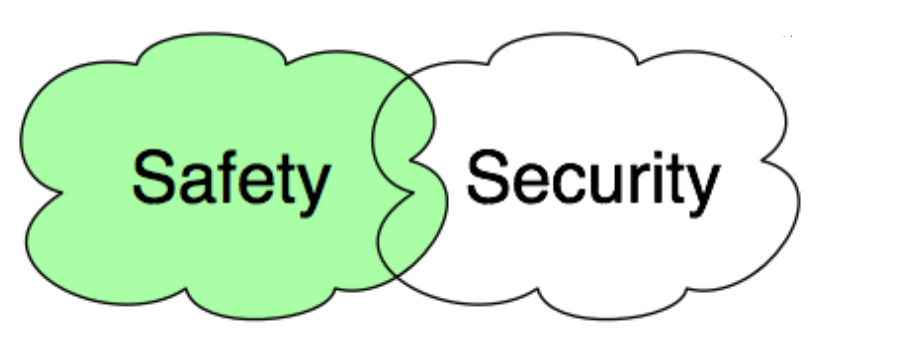
\includegraphics[width=0.7\linewidth]{Pics/SafetyVsSecurity.PNG}
\end{figure}

\begin{itemize}
\item Nicht immer klare Trennung
\item Sicherheit gegen Angriffe (Security) liefert oft auch Sicherheit gegen unbeabsichtigte Fehlbedienung
\item Betriebssicherheit (Safety) vs. Funktionssicherheit
\item Gelegentlich Wiederspruch (Beispiel Fluchttür)
\end{itemize}

\section{Wie viel Sicherhet?}

\begin{figure}[h!]
\centering
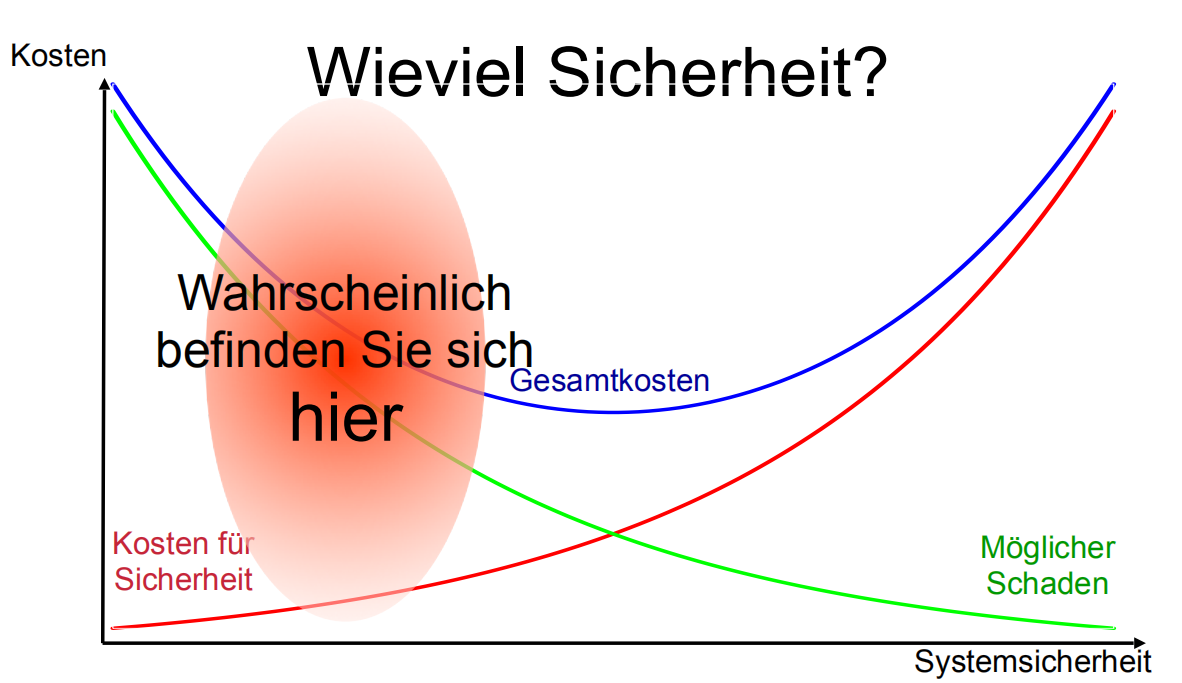
\includegraphics[width=0.7\linewidth]{Pics/HowMuchSecurity.PNG}
\end{figure}

\section{Sicherheitsprobleme}

\begin{itemize}
\item Für ein System bestehen Sicherheitsziele (security objectives)
\item Sicherheitssysteme haben Schwachstellen (weaknesses)
\item Verwundbarkeiten (vulnerabilities) erlauben das Umgehen (oder den Missbrauch) von Sicherheitsmechanismen
\item Eine Bedrohung (threat) ist die Möglichkeit eines Angriffs (attack)
\item Angriffe erzeugen u.U. Schaden (damage)
\item Risiko (Risk) = p(attack) x cost(damage)
\end{itemize}

\section{Sicherheitssysteme}

\begin{itemize}
\item Erfolgreiche Angriffe 
\begin{itemize}
\item Verhindern (prevention)
\item Erkennen (detection)
\item Eingrenzen (Schadensbegrenzung) (containment)
\end{itemize}
\item Sicherheitsregeln (security policy)
\begin{itemize}
\item Richtlinien; Schulung der Mitarbeiter
\item Notfallplanung, -training
\item Management-Unterstützung, Schutz der Sicherheitsverantwortlichen
\end{itemize}
\end{itemize}

\section{Wer sind die Angreifer?}

\begin{itemize}
\item \textbf{Insider} (faul, anders fokussiert, frustriert, kriminell)
\begin{itemize}
\item Eventuell als Folge von \textbf{Social Engineering}
\end{itemize}
\item \textbf{''Hacker''} (richtiger: Cracker), ''script kiddies''
\item \textbf{Professionelle} Angreifer (Spionage, Geheimdienste)
\item Organisiertes \textbf{Verbrechen}
\begin{itemize}
\item Z.B. Erpressung
\item Z.B. Ausschalten eines Kokurrenten, Wirtschaftsspionage
\item Z.B. Beschaffung einer Plattform für weitere Angriffe
\end{itemize}
\end{itemize}

\section{Forensic Readiness}

\begin{itemize}
\item Prevent
\item Detect
\item Contain
\item \textbf{Prosecute} (or at least fend off the inevitable lawsuits)
\end{itemize}

\section{Sicherheitsziele}

\begin{itemize}
\item \textbf{Vertraulichkeit}/Geheimhaltung/Datenschutz - Anonimität
\item \textbf{Integrität}/Authentizität
\item Zurechenbarkeit/Verbindlichkeit
\item \textbf{Verfügbarkeit}
\end{itemize}

\section{Vertraulichkeit/Geheimhaltung/Datenschutz}

\begin{itemize}
\item Vertraulichkeit (confidentiality): Verpflichtung zur Geheimhaltung der Informationen anderer
\item Geheimhaltung (secrecy): Einschränkung des Zugriffs
\item Datenschutz (privacy): Recht auf Schutz eigener (persönlicher) Informationen. 
\end{itemize}

\textbf{Achtung:} Oft ist die Tatsache einer Kommunikationshandlung bereits geheimzuhaltene Information (vs. traffic analysis)

\section{Anonymität}

Anonymität (anonimity): Durchführung von Handlungen ohne Preisgabe der Identität:
\begin{itemize}
\item Eventuell auch Preisgabe eines Pseudonyms
\item Anonymität = Vertraulichkeit der Identität
\end{itemize} 

\section{Integrität/Authentizität}

\begin{itemize}
\item \textbf{Integrität (integrity)} der Daten: Schutz vor unautorisierter und unbemerkter Veränderung von Daten (vgl. Integritätsbegriff aus den Datenbanken). Beispiel: Kontendaten in einer Bank.
\item \textbf{Authentizität (authenticity):} Information ist integer und frisch; eindeutig einer Identität zuzuordnen.
\end{itemize}

\section{Zurechenbarkeit/Verbindlichkeit}

\begin{itemize}
\item Zurechenbarkeit (accountability): Eine durchgeführte Handlung kann einem Kommunikationspartner eindeutig zugeordnet werden.
\item Verbindlichkeit (3rd-party verifiability, 'non-repudiation'): kein unzulässiges Abstreiten durchgeführter Handlungen. Notwendige Beispiele für:
\begin{itemize}
\item Abscließen von elektronischen Kaufverträgen
\item Digital unterschriebene Gerichtsanträge
\end{itemize}
\end{itemize}

\begin{figure}[h!]
\centering
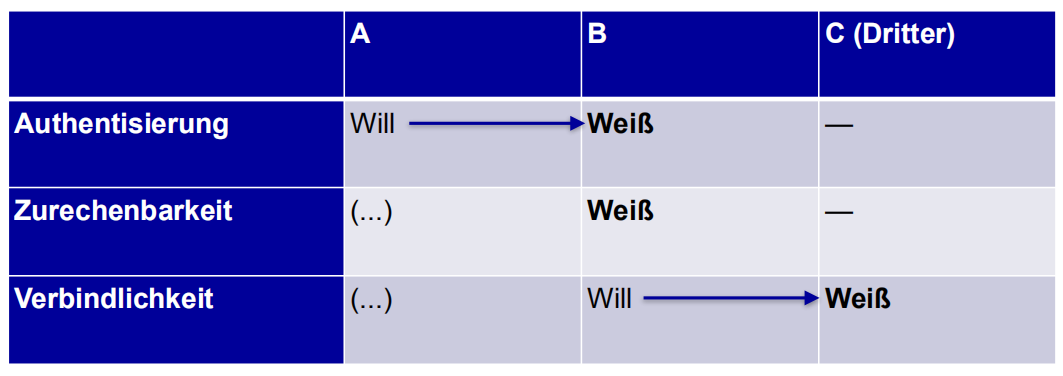
\includegraphics[width=\linewidth]{Pics/Authenticity3rdParty.PNG}
\end{figure}

\newpage

\section{Verfügbarkeit}

\begin{itemize}
\item Verfügbarkeit (availability): Schutz vor unbefugter Beeinträchtigung der Funktionalität von Komponenten, Diensten etc.
\begin{itemize}
\item vs. Denial-of-Service (DoS-) Angriffe
\end{itemize}
\item Ergibt zusammen mit Korrektheit: Verlässligkeit (dependability): Funktionssicherheit; zuverlässige Erbringung der Funktion (reliability)
\end{itemize}

\textbf{Eselsbrücke: CIA}
\begin{itemize}
\item \textbf{C}onfidentiality
\item \textbf{I}ntegrity
\item \textbf{A}vailability
\end{itemize}

\section{Wo liegen die Schwachstellen?}

\begin{itemize}
\item Schlechtes Design: z.B. fehlende Kontrollen, zu grobe Rechtevergabe
\item Schlechte Implementierung: z.B. Pufferüberläufe, schwache Mechanismen, Umgehungswege
\item Schlechte Systemadministratoren: z.B. Account mit Standartpasswort, offene Ports im Firewall, Einsatz ungeeigneter Systeme und Werkzeuge
\item Schlechtes Management: z.B. unklare Sicherheitspolitik, unklare Sicherheitsregeln, fehlendes Sicherheitsbewusstsein der Mitarbeiter, keine Mittel für Sicherheitsüberprüfungen
\end{itemize}

\section{Designprinzipien für sichere Systeme }

\textbf{Saltzer, Schroeder (1975):}
\begin{itemize}
\item \textbf{Priciple of Economy of Machanism:} The protection mechanism should have a simple and small design.
\item \textbf{Principle of Fail-safe Defaults:} The protection mechanism should deny access by default, and grant access only when explicit permission exists.
\item \textbf{Priciple of Complete Mediation:} The protection mechanism should check every access to every object.
\item \textbf{Principle of Open Design:} The protection mechanism should not depent on attackers being ignorant of its design to succeed (no \textbf{security by obscurity}). It may however be based on the attacker's ignorance of specific information such as passwords or cypher keys.
\item \textbf{Principle of Separation of Privilege:} The protection mechanism should grant access based on more than one piece of information.
\item \textbf{Principle of Least Privilege:} The protection mechanism should force every process to operate with the minimum privileges needed to perform its task.
\item \textbf{Principle of Least Common Mechanism:} The protection mechanism should be shared as little as possible among users.
\item \textbf{Principle of Psychological Acceptability:} The protection mechanism should be easy to use (at least as easy as not using it).
\item \textbf{Principle of Defence in Depth:} There should be multiple layers of defense before a high-value target is compromised (No Maginot lines).
\item \textbf{Priciple of Securing the Weakest Link:} The protection mechanism should not have weak spots that allow circumventing the well-secured parts. (Security often is a chain)
\item \textbf{Principle of Reluctance to Trust:} The protection mechanism should not give unwarranted trust to any mechanism or entity. (Healthy spekticism)
\end{itemize}

% Chapter 2
\chapter{Zugriffskontrolle}

\section{AAA}

\begin{itemize}
\item Zugriffskontrolle (\textbf{access control}) regelt: ''\textbf{Wer} darf in einem IT-System auf \textbf{welche} Ressourcen \textbf{wie} zugreifen''.
\item Alternativer Begriff: Autorisierung (\textbf{Authorisation})
\begin{itemize}
\item AAA = Authentication, \textbf{Authorisation}, Accounting (Authentisierung, \textbf{Authorisierung}, Abrechnung)
\end{itemize}
\end{itemize}

\section{Grundbegriffe: Zugriffskontrolle}

\begin{itemize}
\item Subjekt (\textbf{subject}): Initiator der Handlung
\begin{itemize}
\item Benutzer (z.B. Alice, Bob), Gruppen, Prozesse , Rechner/Geräte
\item Genauer: \textbf{principal} als IT-Realisierung einer \textbf{person} oder Funktion
\end{itemize}
\item Objekt (\textbf{object}): Gegenstand der Handlung, Ressource
\begin{itemize}
\item Dateien, SQL-Tabellen, Konto, Prozesse
\item Achtung: Subjekte können auch Objekte sein
\end{itemize}
\item Berechtigung (\textbf{permission}) bzw. Zugriffsrecht (\textbf{access rights}):
\begin{itemize}
\item Was genau darf gemacht werden
\item Z.B.: lesen, schreiben, ausführen, löschen
\end{itemize}
\end{itemize}

\newpage
\section{Unterschiedliche Ebenen der Zugriffskontrolle}

\begin{figure}[h!]
\centering
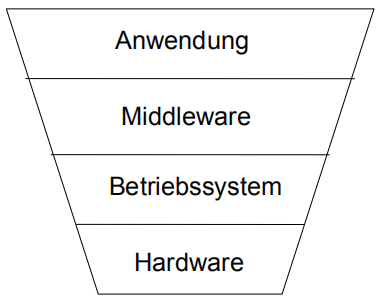
\includegraphics[width=0.5\linewidth]{Pics/AccessControl.PNG}
\end{figure}

\begin{itemize}
\item Abhängigkeit der höheren Ebenen von den Zugriffskontrollmechanismen der niedrigeren Ebenen
\item Zugriffskontrollmechanismen sind in höheren Ebenen komplexer
\item Fehler in niedrigeren Ebenen können zum Umgehen der Sicherheitsmechanismen der höheren Ebenen führen
\end{itemize}

\section{Referenzmonitor}

\begin{figure}[h!]
\centering
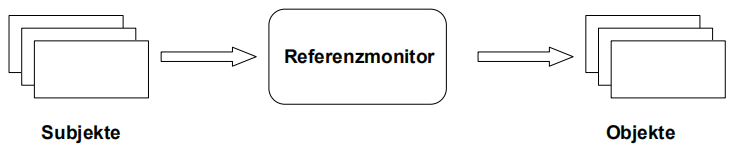
\includegraphics[width=\linewidth]{Pics/ReferenceMonitor.PNG}
\end{figure}

\textbf{Principle of Complete Mediation:} The protection mechanism should check every access to every object.

\section{Zugriffsmatrix (Lampson 1974)} 

\begin{itemize}
\item Zugriffskontrolle wird in ihrer grundlegenden Form dargestellt durch eine Zugriffskontrollmatrix (\textbf{access control matrix}) \textbf{M} mit: $$M:S\times O\rightarrow 2^R$$ wobei \textbf{S} die Mende der Subjekte, \textbf{O} die Menge der Objekte und \textbf{R} die Menge der Zugriffsrechte wie z.B. read,write und execute sind.
\item Subjekt $s$ darf Objekt $o$ genau dann lesen, wenn $\text{read}\in M(s,o)$
\end{itemize}

Beispiel für eine Zugriffsmatrix:

\begin{figure}[h!]
\centering
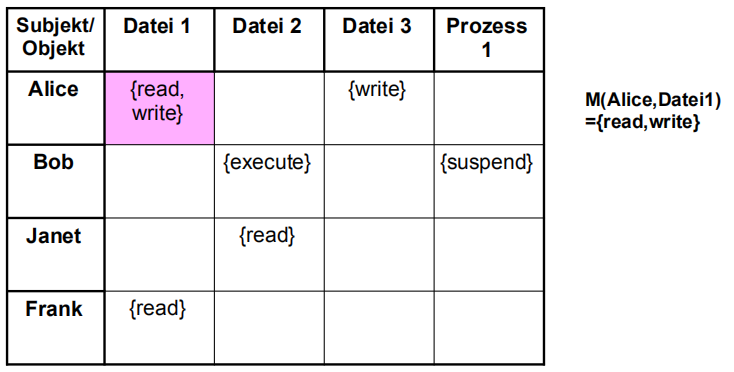
\includegraphics[width=0.85\linewidth]{Pics/AccessMatrix.PNG}
\end{figure}

\section{Zugriffskontrolllisten}

\begin{itemize}
\item Zugriffsmatrix ist oft dünn besetzt, d.h. eine vollständige Speicherung ist zu speicherintensiv $O(|S|\times |O|)$
\item \textbf{Zugriffskontrolllisten (access control lists, ACLs)}: Realisierung der Matrix nach Spalten
\item Subjekte und deren Zugriffsrechte werden \textbf{beim Objekt} gespeichert
\item \textbf{Beispiel:} ACL(Datei1)=((Alice, \{read,write\}),(Frank,\{read\}))
\end{itemize}

\begin{figure}[h!]
\centering
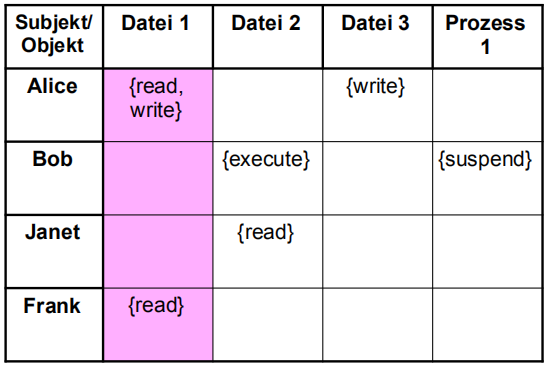
\includegraphics[width=0.7\linewidth]{Pics/AccessControlLists.PNG}
\end{figure}

\begin{itemize}
\item Am häufigsten eingesetztes Konzept für die Zugriffskontrolle im gängigen Betriebssystemen (Windows NT(=2000/XP), Unix/Linux)
\item Vorteile:
\begin{itemize}
\item Vergebene \textbf{Zugriffsrechte} sind effizient für \textbf{Objekte bestimmbar}
\item \textbf{Rechterücknahme} (pro Objekt) ist meist effizient realisierbar
\item Einfach zu implementieren
\end{itemize}
\item Nachteile:
\begin{itemize}
\item Bestimmen der \textbf{Subjekt-Rechte} i.d.R. \textbf{sehr aufwendig} (alle Objekte im System untersuchen)
\item Aufwendige ACL-Kontrollen bei jedem Zugriff
\item \textbf{Schlechte Skalierbarkeit} bei sehr dynamisch wechselnder Menge von Subjekten, falls ACLs \textbf{für einzelne Subjekte/Nutzer} vergeben werden.
\end{itemize}
\end{itemize}

\textbf{Beispiel: Zugriffskontrolle in Unix}

\begin{itemize}
\item Subjekte:
\begin{itemize}
\item Benutzer: User-ID, Group-ID, supplementary Group IDs (bis zu 16)
\item Prozess: User-ID/Group-ID (effective, real, saved), supplementary Group IDs
\end{itemize}
\item Dateien:
\begin{itemize}
\item Owner (User-ID), Group (Group-ID)
\item rwx-bits für: Owner, Group, Other
\item sUid, sGid: Rechteveränderungen bei Dateiaufruf
\end{itemize}
\item Verzeichnisse:
\begin{itemize}
\item Ebenso, plus:
\item t-Bit (nur der Eigentümer darf Dateien in diesem Verzeichnis löschen)
\item sGid-Bit (steuert Gruppe bei Datei-Erzeugung)
\end{itemize}
\item Schutzbits sind einfache Form von ACL
\begin{itemize}
\item Informationen für die Zugriffskontrolle den Dateien zugeordnet
\end{itemize}
\item Schutzbit-ACL so nicht feingranular genug:
\begin{itemize}
\item Alive kann nicht \textbf{Bob allein} nur Lese-Rechte auf eine bestimmte Datei geben
\item Uni Bremen: ''grp'' zur Einrichtung von Gruppen durch Benutzer
\end{itemize}
\item FreeBSD, Solaris haben zusätzliches ACL-Konzept
\item POSIX-Kommandos: getfacl, setfacl
\begin{itemize}
\item Und chmod-Erweiterungen: +a/-a/=a
\end{itemize}
\end{itemize}

\newpage

\section{FreeBSD-ACLs (POSIX .1e)}

\begin{itemize}
\item Menge von Tripeln Typ:Name:Rechte
\begin{itemize}
\item user::rwx  (Dateieigner)           1
\item group::r-x (Gruppe der Datei)  2
\item other::r-x  (Der Rest)               5
\end{itemize}
\item Neu:
\begin{itemize}
\item user:fritz:r-x         (spezifischer Benutzer) 2
\item group:katzen:rwx (spezifische Gruppe)     4
\end{itemize}
\item Einschränkungen über \textbf{Maske} (chmod-Kompatibilität)
\begin{itemize}
\item mask::r-x (schränkt alles außer 1 und 5 ein)
\end{itemize}
\end{itemize}

\section{NFSv4-ACLs}

\begin{itemize}
\item Allgemeiner Nachfolger der POSIX-ACLs
\item Liste von ACEs (Access Control Entry)
\begin{itemize}
\item 17 permission bits, 4 inheritance flags
\end{itemize}
\item Triviale ACL: Wie traditionelles UNIX
\begin{figure}[h!]
\centering
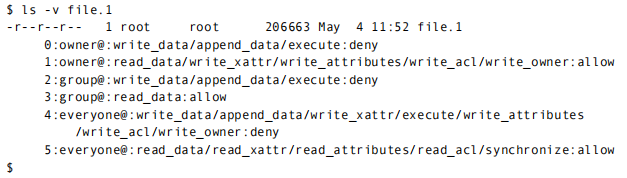
\includegraphics[width=\linewidth]{Pics/NFSACLs.PNG}
\end{figure}
\item Kommandos: ls -v, chmod -A
\end{itemize}

\section{Windows-ACLs}

\begin{itemize}
\item Zugriffsrechte auf Dateien, Ordner oder Drucker werden mit \textbf{Access Control Lists} verwaltet.
\item Pro \textbf{Objekt}:
\begin{itemize}
\item Security identification number (SID) als Bezeichner für \textbf{Eigner} (owner)
\item \textbf{ACL}
\end{itemize}
\item ACL besteht aus einzelnen Access Control Entries (ACEs):
\begin{itemize}
\item Typ der ACE (Erlauben, Verweigern, Überwachen)
\item Subjekt (Benutzer oder Gruppe), für den/die der ACE gilt
\begin{itemize}
\item SID als Bezeichner für Subjekt
\end{itemize}
Berechtigungen, für die der ACE gilt (Bitmaske) \\ Vererbbarkeit der ACE auf Unterobjekte
\end{itemize}
\end{itemize}

\begin{itemize}
\item ACL:
\begin{figure}[h!]
\centering
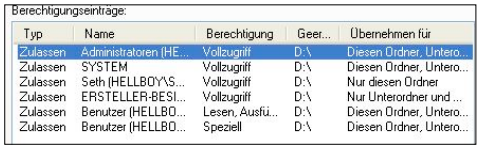
\includegraphics[width=0.75\linewidth]{Pics/WACL1.PNG}
\end{figure}
\item Vererbbarkeit:
\begin{figure}[h!]
\centering
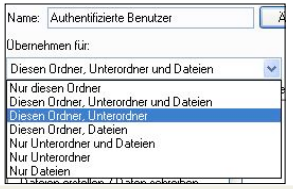
\includegraphics[width=0.5\linewidth]{Pics/WACL2.PNG}
\end{figure}
\item Besitzer hat immer Vollzugriff
\begin{itemize}
\item Besitzer kann auch eine Gruppe sein
\end{itemize}
\item Alle ACEs werden in Reihenfolge ausgewertet
\newpage
\begin{figure}[h!]
\centering
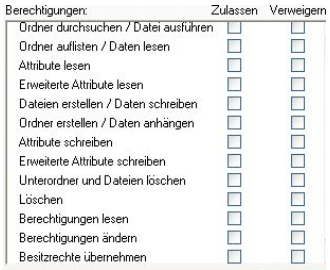
\includegraphics[width=0.5\linewidth]{Pics/WACL3.PNG}
\end{figure}
\item GUI: Deny hat Vorrang vor Allow-Regeln
\begin{itemize}
\item \textbf{Vorsicht}: Verbietet man einer Gruppe alles, gibt es keine möglichkeit, Einzelnen Rechte zu geben!
\end{itemize}
\end{itemize}

\section{Capabilities}

\begin{itemize}
\item \underline{Zeilenweise} Realisierung der Matrix
\item Capability, \underline{Zugriffsticket} mit Objekt-ID und Rechtebits
\item Capability-Besitz berechtigt zur Wahrnehmung der Rehte
\item Für jedes Subjekt \textbf{s} eine Capability-Liste (CList) \\ \textbf{Beispiel:} Clist (Alice) = ((Datei1, \{read,write\}), (Datei3, \{write\}))
\begin{figure}[h!]
\centering
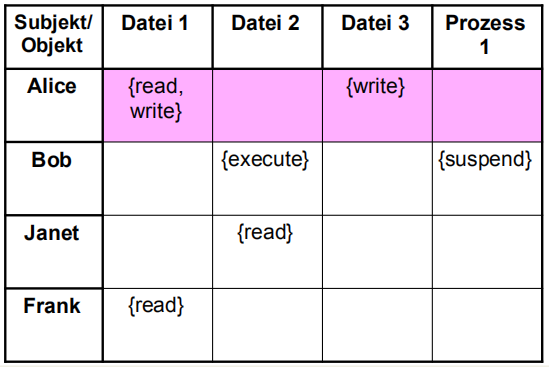
\includegraphics[width=0.7\linewidth]{Pics/CapabilityACL.PNG}
\end{figure}
\item Beispiele von Systemen mit Capability-Konzept: IBM System/38, Mach-$\mu$-Kern (Ports), Amoeba
\item UNIX: File Descriptor = flüchtige Capability
\begin{itemize}
\item Deskriptor-Tabelle in User-Structure = C-List
\item Übergabe von Deskriptoren +ber UNIX-Domain-Sockets
\end{itemize}
\item Achtung: \textbf{Keine} Capabilities in diesem Sinne: ''POSIX Capabilities'' (z.B. von Linux 2.2 unterstützt)
\begin{itemize}
\item Besseres Wort: Privileges
\end{itemize}
\item Renaissance des Capability-Konzeptes durch Zertifikate (X.509, später in VL)
\end{itemize}

\textbf{Vorteile:}
\begin{itemize}
\item Einfache Bestimmung der \underline{Subjekt-Rechte}
\item \underline{Einfache Zugriffskontrolle}: nur noch Ticketkontrolle!
\item \underline{Einfache Delegation} von Rechten anderer Benutzer/Subjekte
\end{itemize}

\textbf{Nachteile:}
\begin{itemize}
\item \underline{Rechterücknahme} schwierig (Ticket aus der Hand)
\item \underline{Keine Subjekt-Ticket Kopplung}, Besitz berechtigt automatisch zur Wahrnehmung der Rechte
\item \underline{Objekt-Sicht auf Rechte schwierig}: Wer darf was?
\end{itemize}

\textbf{Bis hierher: DAC (Discretionary Access Control)}

Bislang:
\begin{itemize}
\item \textbf{Subjekte} entscheiden über die Zugriffsberechtigungen (vgl. chmod in UNIX/Linux oder Dialogsgenster zur Rechtevergabe in Windows 2000/XP)
\item Subjekt bestimmt weitergehend die Security Policy für ''seine'' Objekte (\textbf{benutzerbestimmte Zugriffskontrolle bzw. discretionary access control})
\end{itemize}

\section{Mandatory Access Control (MAC)}
\begin{itemize}
\item In besonders sicherheitskritischen Bereichen mit z.B. hohen Anforderungen an die Vertraulichkeit ist benutzerbestimmte Zugriffskontrolle nicht angemessen
\begin{itemize}
\item Typische Beispiele: Militär, Geheimdienste
\end{itemize}
\item Einführung geeigneter Modelle, die \textbf{vom System} umgesetzt wereden
\item Systembestimmte Zugriffskontrolle (\textbf{Mandatory Access Control})
\item Bekanntestes Beispiel für Mandatory-Access-Control: \textbf{Bell-LaPadula-Modell}
\end{itemize}

\section{Bell-LaPadula-Modell (BLP)}

\begin{itemize}
\item David Bell und Len LaPadula, 1973: auf Initiative der US Air Force \\
\item Zweck:
\begin{itemize}
\item Einfache Sicherheitsmechanismen für die Verifikation
\item Formales Sicherheitsmodell
\item Beschränkung des Informationsflusses, d.h. Sicherheitsziel ist die \textbf{Vertraulichkeit}
\end{itemize}
\end{itemize}

\subsection{Konzepte}

Ein vereinfachtes BLP-Modell:
\begin{itemize}
\item Multilevel Security System (MLS)
\begin{itemize}
\item Alle Subjekte und Objekte erhalten eine \underline{Sicherheitsmarkierung} (\textbf{label}) gemäß der Stufe ihrer Vertraulichkeit wie z.B. top secret > secret > confidential > unclassified
\item Idee: Höher klassifizierte Daten fürfen nur von Mitarbeitern mit einer ausreichenden Sicherheitsstufe gelesen werden
\end{itemize}
\item Formalisierung der Idee:
\begin{itemize}
\item \textbf{M} sei die Zugriffsmatrix
\item \textbf{SC} sei eine Menge von Sicherheitsmarkierungen, und auf \textbf{SC} gelte eine partielle ordnung $\leq $
\item $o\in O:\, SC(o)\in SC$ sei die Sicherheitsmarkierung von Objekt o (\textbf{classification})
\item $s\in S: \, SC(s)\in SC$ sei die Sicherheitsmarkierung von Subjekt s (\textbf{clearance}) \\
\item \textbf{Simple Security-Property (no read-up): \\ $\forall s \in S.\, \forall o \in O: \, \text{read}\in M(s,o)\Rightarrow SC(o)\leq SC(s)$}
\end{itemize}
\item Die no-read-up-Regel reicht nicht: \textbf{Trojanische Pferde} könnten höher klassifizierte Daten einfach nach unten schreiben
\item Die entscheidende Neuerung des BLP-Modelles ist mithin die zweite Regel: \\ \textbf{*-Property (no-write-down): $$\forall s\in S.\, \forall o \in O:\, \text{write}\in M(s,o)\Rightarrow SC(s)\leq SC(o)$$}
\item Manchmal fordert man auch, dass sich die Sicherheitsmarkierungen weder für Objekte noch für Subjekte yur Systemlaufzeit ändern (\underline{Strong Tranquility Property})
\end{itemize}

\textbf{Beispiele: BLP}
\begin{itemize}
\item Viele \underline{Betriebssysteme bieten BLP-Erweiterungen}: u.a. Sun Trusted Solaris 7, Trusted HP-Unix, Linux-Derivate
\begin{itemize}
\item Erweiterter Referenz-Monitor zur Überprüfung der BLP-Regeln
\end{itemize}
\item Daten-Diode (-''Pumpe'')
\begin{itemize}
\item Daten können über ein Kommunikations-Device (Daten-Diode) \textbf{von Low nach High} transferiert (gepumpt) werden, aber nicht in der umgekehrten Richtung 
\item Beispiel: NRL-Pump (US Naval Research Laboratory), 1993
\end{itemize}

\textbf{Fazit: BLP}

\begin{itemize}
\item Stärken:
\begin{itemize}
\item Einfach zu Implementieren (Anpassung des Referenzmonitors)
\item Formales Modell (man kann Sätze über Eigenschaften beweisen)
\item Gut geeignet zum \underline{Nachbilden hierarchischer Informationsflüsse:} z.B. beim Militär, Geheimdienst
\end{itemize}
\item Schwächen:
\begin{itemize}
\item Beschränkte Ausdrucksfähigkeit: keine Integrität (blindes Schreiben)
\item Keine Modellierung von verdeckten Kanälen (\textbf{covert channels}), über die Informationen dann doch unberechtigt fließen können.
\end{itemize}
\end{itemize}
\end{itemize}

\textbf{Verdeckte Kanäle}

\begin{itemize}
\item Zugriffskontrolle schützt den Datencontainer, nicht die Information
\begin{itemize}
\item Möglichkeit von verdeckten Kanälen
\end{itemize}
\item Verdeckte Kanäle (\textbf{covert channels}): \\ Informationsfluß über einen Kanal, der nicht explizit zur Informationsübertragung vorgesehen ist \\ \\ \textbf{Beispiele:}
\begin{itemize}
\item Ressourcen-Konflikt: High-Level-Prozess erzeugt eine Datei, so dass ein Low-Level-Prozess eine Fehlermeldung erhält, wenn die Datei mit gleichem Namen erzeugt wird (1 Bit Information)
\item High-Level-Prozess kann gemeinsam genutzte Ressourcen (Position des Festplattenkopfes, Inhalt des Caches) in einem Zustand hinterlassen, so dass der Low-Level-Prozess anhand von Antwortzeiten zusätzliche Informationen gewinnen kann 
\end{itemize}
\end{itemize}

\newpage

\textbf{Wiederholung: MAC und BLP}

\begin{itemize}
\item MAC: Systembestimmte Zugriffskontrolle (mandatory access control)
\item Bekanntestes Beispiel für MAC: \textbf{Bell-LaPadula}-Modell (BLP)
\item Idee:
\begin{itemize}
\item Klassifizierung von Subjekten und Objekten mit \textbf{Labels}
\item \textbf{Simple Security-Property} (No read-up-Regel)
\item \textbf{*-Property} (No write-down-Regel)
\end{itemize}
\end{itemize}

\textbf{Weiteres MAC-Beispiel: Chinese Wall-Modell}

\section{Chinese Wall-Modell}

\begin{itemize}
\item Brewer und Nash, 1989
\item Modell aus dem Finanzbereich
\item Ausgangssituation:
\begin{itemize}
\item Berater sind für verschiedene Unternehmen/Organisationen (z.B. Banken, Ölfirmen) tätig
\item Insiderwissen darf nicht genutzt werden
\end{itemize}
\end{itemize}

\subsection{Interessenkonflikte}

\begin{itemize}
\item Vermeidung von \textbf{Interessenkonflikten (conflict of interest, COI)}: \\ Ein Berater darf nicht mehrere Firmen/Organisationen aus derselben \textbf{Konfliktklasse (COI class)} beraten
\item Beispiele für Konfliktklassen:
\begin{itemize}
\item Beispiele: Banken, Ölfirmen
\end{itemize}
\end{itemize}

\subsection{Begrifflichkeiten}

\begin{itemize}
\item Drei Arten von Begrifflichkeiten (hierarchische Strukturierung der Daten):
\begin{itemize}
\item 1. \textbf{Objekte} wie in BLP, Zugriffsrechte read, write
\item 2. Objekte gehören eindeutig zu Firmen/Organisationen
\begin{itemize}
\item Menge der Firmdaten: \textbf{Company Data Set (CD)}
\item \textbf{CD(o)} gibt das eindeutige Company Data Set von Objekt \textbf{o} an
\end{itemize}
\item 3. Firmen/Organisationen gehören eindeutig \textbf{Konfliktklassen (COIs)} an
\begin{itemize}
\item COIs enthalten also die CDs der dazugehörigen Firmen/Organisationen
\end{itemize}
\end{itemize}
\end{itemize}

\newpage

\textbf{Beispiel}

\begin{figure}[h!]
\centering
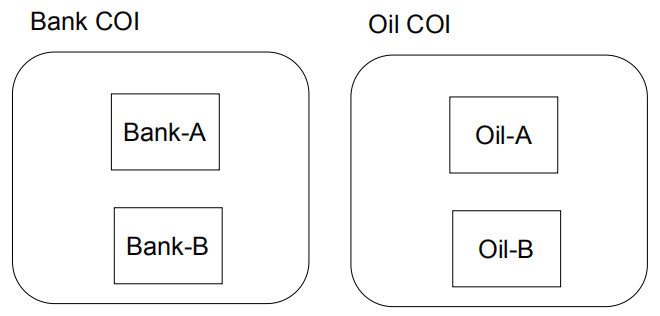
\includegraphics[width=0.85\linewidth]{Pics/COIs.PNG}
\end{figure}

\subsection{Simple Security Property}

\begin{itemize}
\item \textbf{Simple Security Property:} \\ Ein Berater darf auf ein Objekt o lesend zugreifen, nur falls eine der folgenden Bedingungen erfüllt ist:
\begin{itemize}
\item 1. Der Berater hat schon auf andere Objekte dieser Firma/Organisation zugegriffen oder
\item 2. Das Objekt gehört zu einer Konfliktklasse, für die der Berater noch kein Objekt gelesen hat
\end{itemize}
\item Berücksichtigung der \textbf{Zugriffshistorie}; Aufbau einer Chinese Wall
\end{itemize}

\textbf{Beispiel}

\begin{itemize}
\item Ausgangssituation
\begin{itemize}
\item Bank-A und Bank-B
\item Oil-A und Oil-B
\item Alice und Bob sind Berater
\item Annahme: Bob berät Bank-B und hat noch nie eine Ölfirma beraten
\end{itemize}
\item Auf die folgenden Objekte darf Bob dann noch lesend zugreifen:
\begin{itemize}
\item Alle Objekte von Oil-A oder Oil-B
\item Alle Objekte von Bank-B (aber nicht von Bank-A)
\end{itemize}
\end{itemize}

\newpage

\textbf{Reicht die Simple Security-Regel aus?}

\begin{itemize}
\item \textbf{Beispiel:}
\begin{itemize}
\item Bob berät Bank-B und \underline{Oil-A};
\item Alice berät Bank-A und \underline{Oil-A}.
\item Alice hat insbesondere auch \underline{Schreibrechte auf Objekte aus Oil-A}.
\item Simple Security-Regel gilt offenbar.
\end{itemize}
\item Ein \underline{Trojanisches Pferd} könnte Informationen über Bank-A von Alice nach Oil-A kopieren.
\begin{itemize}
\item Bob hat nun mittels Oil-A Zugriff auf diese Informationen.
\item Bob hat also auf Objekte aus Bank-B und (indirekt) Bank-A Zugriff.
\end{itemize}
\item Vergleicdh mit der Problematik ''Verdeckte Kanäle''
\item Einführung einer neuen Regel erforderlich
\end{itemize}

\subsection{Chinese Wall-Modell: *-Property}

\begin{itemize}
\item \textbf{*-Property}: Ein Berater hat schreibenden Zugriff auf ein Objekt \textbf{o}, wenn er bislang nur Objekte aus der Firma von Objekt \textbf{o}, aber keine anderen gelesen hat.
\item Für unser Beispiel bedeutet dies: Alice darf \textbf{nicht} Objekte in Klasse \underline{Oil-A} schreiben, weil sie lesenden Zugriff auch auf Objekte aus \underline{Bank-A} besitzt.
\end{itemize}

\subsection{Bewertung/Einordnung}

\begin{itemize}
\item Chinese Wall-Modell zugeschnitten auf bestimmte Problematik aus dem Finanzbereich
\item Nur Vertraulichkeit, keine Integrität
\item Umsetzung durch organisatorische Maßnahmen und weniger durch IT-Systeme
\end{itemize}

\section{Andere Modelle für Zugriffskontrolle}

\begin{itemize}
\item \textbf{Biba}-Modell (Ken Biba, 1977), Integrität (aber kein Informationsfluß)
\begin{itemize}
\item Ab MS-Vista enthält Windows Biba-Konzepte (z.B. Beschränkung von Änderungen von Registry-Einträgen)
\end{itemize}
\item \textbf{Clark-Wilson} (David Clark, David Wilson, 1987): Sicherheitsmodell für Banken- und Buchhaltungsprogramme
\item \textbf{Non-Interference-Modelle} (z.B. Meseguer, Goguen, 1982): $\rightarrow$ Verdeckte Kanäle
\item Domain Type Enforcement
\end{itemize}

\section{Domain-Type-Enforcement (DTE)}

\begin{itemize}
    \item Beobert und Kain, 1985
    \item \textbf{Idee:}
    \begin{itemize}
        \item Zuordnung von Objekten (z.B. Dateien, Sockets, Prozesse) zu \textbf{Typen}
        \item Zuordnung von Subjekten (z.B. Nutzer, Prozesse) zu \underline{Domains}
    \end{itemize}
    \item Zusätzliche Zugriffsmatrix
    \begin{itemize}
        \item nicht für einzelne Objekte und Subjekte, sondern für \textbf{Typen} und \textbf{Domains}
    \end{itemize}
\end{itemize}

\textbf{Beispiel: M(admin\textunderscore d, writeable\textunderscore t) = \{create, write, read, search\}} 

\begin{itemize}
    \item Vertraulichkeit und Integrität
    \item Anwendung: SELinux
\end{itemize}

\section{Rollenbasierte Zugriffskontrolle}

\begin{itemize}
    \item \textbf{Idee der rollenbasierten Zugriffskontrolle (role-based access control, RBAC):} \\ Knüpfung der Rechte nicht mehr direkt an Benutzer, sondern an \textbf{Rollen (roles)}
    \item Rollen entsprechen häufig \textbf{Funktionen/Aufgaben}, die in einer Organisation (Krankenhaus, Bank, Behörden, Unternehmen) auftreten
    \item Geeignet für hierarchisch aufgebaute Organisationen
    \item Andere Form von MAC
    \item Beispiel: Bank
    \begin{itemize}
        \item Kassierer, Kassenprüfer, Zweigstellenleiter
    \end{itemize}
    \item State-of-the-Art!
\end{itemize}

\subsection{RBAC gemäß ANSI-Standard}

\begin{itemize}
    \item ANSI-Standard für RBAC (ANSI-INCITS 359-2004)
    \item Entitäten des ANSI-Standards für RBAC:
    \begin{itemize}
        \item \textbf{Benutzer (users)} sind für Personen (und keine Prozesse, vgl. Subjekt-Begriff)
        \item \textbf{Zugriffsberechtigung (permissions)} sind paare (Operation,Subjekt). \\ Beispiele: (read,File1), (read,File2), (debit, account1), (credit, account2)
        \item Eine \textbf{Rolle} ist eine Sammlung von Zugriffsberechtigungen
    \end{itemize}
    \item Rollen werden Benutzern zugewiesen. Eine Rolle ist also \underline{Mittler} zwischen Benutzern und Berechtigungen.
    \item Rollen werden von Benutzern in \textbf{Sitzungen (sessions)} aktiviert.
    \begin{itemize}
        \item Unterscheidung von Rollenzuweisung und -aktivierung. Welches Sicherheitsprinzip?
        \item Least Privilege
    \end{itemize}
    \item Formalisierung?
\end{itemize}

\subsection{Formalisierung von RBAC gemäß ANSI-Standard}

\begin{itemize}
    \item \textbf{Mengen}:
    \begin{itemize}
        \item Users, Roles, Permissions, Sessions
    \end{itemize}
    \item \textbf{Relationen:}
    \begin{itemize}
        \item UA $\subseteq$ Users $\times$ \underline{Roles} \textbf{user assignment} \\ Zuordnung von Benutzern zu Rollen
        \item PA $\subseteq$ Permissions $\times$ \underline{Roles} \textbf{(permission assignment)} \\ Zuordnung von Zugriffsberechtigungen zu Rollen
        \item RBAC soll Organisationsstrukturen nachbilden, also Einführung von Rollenhierarchien \textbf{(role hierarchies)}: \\ RH $\subseteq$ Roles $\times$ Roles, RH ist eine partielle Ordnung auf Roles $\times$ Roles
    \end{itemize}
    \item \textbf{Funktionen:} \\ session\textunderscore user : Sessions $\rightarrow$ User - eindeutiger Besitzer einer Sesssion \\ session\textunderscore roles $\rightarrow 2^\text{Roles}$ - die in einer Session aktivierten Rollen
\end{itemize}

\newpage

\subsection{Komponenten von RBAC}

\begin{figure}[h!]
    \centering
    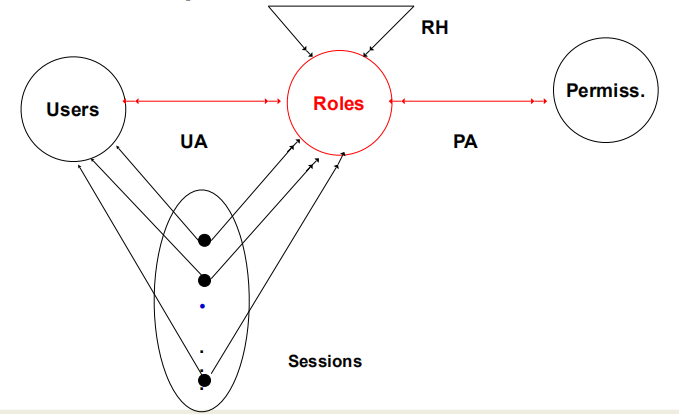
\includegraphics[width=0.85\linewidth]{Pics/RBAC.PNG}
\end{figure}

\textbf{Rollenhierarchie: Beispiel}

\begin{figure}[h!]
    \centering
    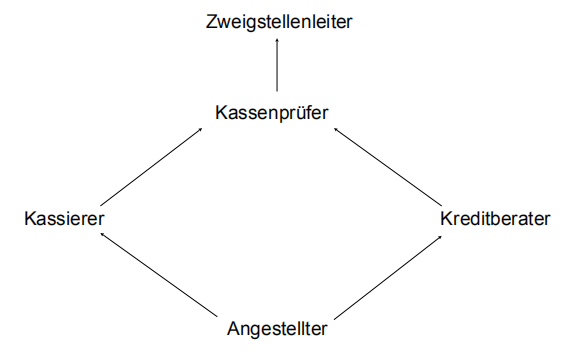
\includegraphics[width=0.55\linewidth]{Pics/RBAC_EXAMPLE.PNG}
\end{figure}

\textbf{Warum vereinfacht RBAC das Berechtigungsmanagement?}

\begin{figure}[h!]
    \centering
    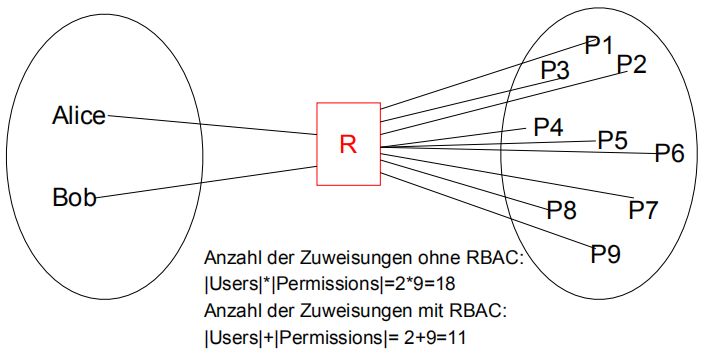
\includegraphics[width=0.85\linewidth]{Pics/RBAC2.PNG}
\end{figure}

\subsection{Erweiterung von RBAC: Separation of Duty}

\subsubsection{Motivation}

\begin{itemize}
    \item Niedergang der Barings-Bank, 1995 \\ ''In a fatal mistake, the bank allowed Leeson to remain Chief Trader while being responsible for settling his trades, a job that is usually split. This had made it much simpler for him to hide his losses.'' \\ \\ ''Der Starhändler musste keine Rechenschaft über seine Transaktionen geben, eine Compliancestelle oder eine eigene Abwicklungsabteilung gab es nicht. Im Grunde kontrollierte sich Leeson weitgehend selbst.'' ARD, 27.02.2020, 25 Jahre später
    \item Ähnlicher Fall, aber mit etwas geringeren Folgen: Betrug bei der Société Générale, Jérôme Kerviel, 2008
\end{itemize}

\subsection{Saperation of Duty (SoD)}

\begin{itemize}
    \item Separation of Duty (SoD) - \textbf{Aufgabentrennung}
    \begin{itemize}
        \item Manchmal auch ''Vieraugen-Prinzip'' gennant
    \end{itemize}
    \item Natürliche Abbildung von \textbf{organisationsinternen Kontrollregeln} mittels RBAC
    \item Beispiele für die Aufgabentrennung:
    \begin{itemize}
        \item Die Rollen \textbf{Kassenprüfer} und \textbf{Kassierer} dürfen nicht von ein und derselben Person angenommen werden.
        \item Trennung der Rollen \textbf{Kunde} und \textbf{Kreditberater}
    \end{itemize}
\end{itemize}

\subsection{Statische Separation of Duty}

\begin{itemize}
    \item Im RBAC-Formalismus: \\ \\ \textbf{CR} (Menge von Konfliktrollen) - z.B. CR=\{Kassierer, Kassenprüfer\} \\ \\ \textbf{roles(u)} $=\{ r\in R\, |\, (u,r)\in UA\}$ - Rollen von u \\ \\ \textbf{Statische Separation of Duty:} $$\forall u\in \text{User:} \, |roles(u)\cap CR|\leq 1$$ ''User u darf höchstens eine Konfliktrolle annehmen''.
    \item Darf ein \textbf{Kreditberater} auch \textbf{Kunde} in der Bank sein, in der er arbeitet?
    \begin{itemize}
        \item Einführung von dynamischer SoD
    \end{itemize}
\end{itemize}

\subsection{Dynamische Separation of Duty}

\begin{itemize}
    \item Trennung von Rollen nicht beim UA, sondern beim Aktivieren von Rollen in Sitzungen (flexibler als statische SoD)
    \item Im RBAC-Formalismus: \\ \\ \textbf{active\textunderscore roles(u)} $$=\{ r\in R\, | \, (u,r)\in UA\wedge \forall s\in S.(\text{user}(s)=u\wedge r\in \text{session\textunderscore roles}(s))\}$$ \\ \textbf{Dynamic Separation of Duty:} \\ $$\forall u \in \text{User}: \, | \text{active\textunderscore roles}(u)\cap CR|\leq 1$$ \\ ''User u darf höchstens eine Konfliktrolle \textbf{aktivieren}''.
\end{itemize}

\subsection{Authorization Constraints}

\begin{itemize}
    \item Statische und dynamische SoD sind Ausprägungen des allgemeineren Konzepts der \textbf{Authorization Contraints}.
    \item Rollenbasierte Authorization Constraints sind Einschränkungen der Rollenrelationen und drücken \textbf{organisatorische Regeln} aus
    \item Andere Formen von rollenbasierten Authorization Constraints:
    \begin{itemize}
        \item Verschiedenste (teilweise applikationsanhängige) SoD-Beschränkungen:
        \begin{itemize}
            \item Object-based Dynamic SoD: Ein Mitarbeiter aus der Finanzabteilung eines Unternehmens darf nicht gleichzeitig eine Bestellung vorbereiten \textbf{und dann} genehmigen
            \item Werden oft im Workflow-Kontext verwendet 
        \end{itemize}
        \item Kardinalitätsbeschränkungen
        \item Prerequisite Roles
        \item Temporale Beschränkung
    \end{itemize}
\end{itemize}

\subsection{Einsatzgebiete von RBAC}

\begin{itemize}
    \item Betriebssysteme (RACF von IBM, Windows NT/2000/7/10 zumindest als Gruppenkonzept, SELinux - später)
    \item Middleware (z.B. Web Services)
    \item Rollenbasierte Administrationswerkzeuge wie z.B. DirXMetaRole von Simens oder IBM Tivoli
    \item Datenbanken (z.B. Oracle, Sybase, Informix)
    \item Enterprise Resource Planning Systeme wie z.B. SAP
    \item Krankenhausinformationssysteme, Bankenanwendungen (weitere Verbreitung im Bankbereich), E-Goverment
\end{itemize}

\subsection{Stärken}

\begin{itemize}
    \item Rollenkonzepte sind \textbf{flexibel verwendbar}
    \item \textbf{Vereinfachtes Berechtigungsmanagement} (wenn bspw. Benutzer häufig wechseln, dann braucht i.d.R. nur die Relation UA angepasst zu werden)
    \item Abbildung von \textbf{hierarchischen Organisationsstrukturen}
    \item Intuitive Abbildung auf Geschäftsprozesse
    \item Möglichkeit, \textbf{organisationsinterne Sicherheits- und Kontrollregeln} abzubilden (Authorization Constraints)
    \item Sowohl \textbf{Vertraulichkeit} als auch \textbf{Datenintegrität} (BLP kann durch RBAC simuliert werden)
\end{itemize}

\subsection{Schwächen}

\begin{itemize}
    \item Woher bekommt man überhaupt die Rollen, die für eine Organisation relevant sind? (Problem des \textbf{Role Engineering})
    \item Automatische Zuweisung von Berechtigungen zu Rollen wird nicht ausreichend unterstützt (manuelle Zuweisung in großen Organisationen nicht praktikabel)
    \item Rollenproliferation (Beispiele: Krankenhaus mit 300 Rollen, Verwaltung der Universität: 800 SAP-Rollen)
    \begin{itemize}
        \item Faustregel: $|$Roles$|$/$|$User$|$=0.04 (20,000 Mitarbeiter der Verwaltung?!)
    \end{itemize}
    \item Viele Projekte zur Einführung von RBAC scheitern aus o.g. Gründen
    \item Kein Schutz gegenüber Covert channels (wie bei allen Modellen für die Zugriffskontrolle)
\end{itemize}

\section{SELinux - Security Enhanced Linux}

\begin{itemize}
    \item Von der NSA (National Security Agency) entwickelt, 2001
    \item Erweiterung von Linux um MAC-Konzepte; frei verfügbar
    \item Unterstützung von SUSE-, Debian-, Ubuntu-Linux, auch von Android
    \item Mittlerweise Einsatz in britischen Behörden, um BLP-artige Zugriffskontrolle umzusetzen
\end{itemize}

\subsection{Ziele}

\begin{itemize}
    \item \textbf{Konfigurierbare} Sicherheitsrichtlinien (\textbf{security policies}) für die Zugriffskontrolle, u.a.:
    \begin{itemize}
        \item RBAC
        \item BLP
        \item Chinese-Wall
        \item Biba
        \item Clark-Wilson
        \item Eigene, organisationsabhängige Security policies
    \end{itemize}
    \item Trennung von Definition und Durchsetzung (\textbf{enforcement}) der Sicherheitsrichtlinien
    \item Trennung von Prozessen
\end{itemize}

\subsection{Konzepte}

Drei Zugriffskontrollkonzepte/-modelle:
\begin{itemize}
    \item 1. DTE als Basis:
    \begin{itemize}
        \item Der Einfachheit halber aber keine Domains, sondern nur Typen
    \end{itemize}
    \item 2. RBAC:
    \begin{itemize}
        \item Kein PA, sondern Zuordnung von DTE-Typen zu Rollen
        \item UA wie immer
        \item Auch Unterstützung von Authorization Constraints
    \end{itemize}
    \item 3. IBAC (identity-based access control)
    \begin{itemize}
        \item Jeder Prozess behält seine ID: im Gegensatz zum s-Bit in Linux
    \end{itemize}
\end{itemize}

\subsection{Sicherheitsarchitektur}

\begin{itemize}
    \item Sicherheitsrichtlinien werden in verschiedenen Textdateien definiert
    \item Integration eines \textbf{Security Servers} in den Linux-Kernel
    \item Laden der Sicherheitsrichtlinien beim Start in den Kernel
    \begin{itemize}
        \item Dynamisches Nachladen von Sicherheitsrichtlinien möglich
    \end{itemize}
    \item Überprüfung von Zugriffen durch den Security Server:
    \begin{itemize}
        \item Werden beim Zugriff die definierten Sicherheitsrichtlinien verletzt?
        \item Security Server als API, der Rest des Kernels ruft diesen auf (enforcement)
        \item Subjekte und Objekte haben \textbf{Security Identifier} (SID), die bei der Überprüfung verwendet werden
        \item SID: Handler auf \textbf{Security Kontext}, der die eigentlichen Sicherheitsinformationen (Rolle, UserID, Typen...) enthält (Indirektion)
    \end{itemize}
\end{itemize}

\subsubsection{Wie sehen Sicherheitsrichtlinien in SELinux aus?}

\begin{itemize}
    \item DTE-Zugriffsmatrix \\ \textbf{allow type\textunderscore 1 type\textunderscore 2:class \{perm\textunderscore 1 ... perm\textunderscore n\}} \\ \textbf{allow user\textunderscore t tmp\textunderscore t:dir \{read search add\textunderscore name remove\textunderscore name\}} \\ ''Jeder Nutzer kann im /tmp-Verzeichnis Dateien erzeugen und löschen''
    \item User Assignments \\ \textbf{user username roles \{role\textunderscore 1, ..., role\textunderscore n\}}
    \item Type Assignments \\ \textbf{role rolename types \{type\textunderscore 1, ..., type\textunderscore n\}}
    \item Zusätzlich: Datei für Authorization Constraints
\end{itemize}

\subsection{Abschließende Anmerkungen}

\begin{itemize}
    \item Erhöhte Sicherheit durch: MAC-Unterstützung, Trennung von Prozessen, kein s-Bit
    \item Kompatibilität zu Linux-Distributionen/-Derivanten, z.B. SUSE, Debian, Android (Ubuntu setzt eher auf AppArmor)
    \item Flexible Konfigurationsmöglichkeiten von Sicherheitsrichtlinien (aber Dateien mit Sicherheitsregeln gut schützen!)
    \item \underline{Nachteil:} Komplexität der Policy-Definition
    \begin{itemize}
        \item Werkzeuge zur Policy-Analyse wünschenswert, Usability-Aspekt
        \item Vorgegebene Policy-Definitionen
    \end{itemize}
    \item Mehr über SELinux: https://github.com/SELinuxProject
\end{itemize}

\section{Sandboxing}

\begin{itemize}
    \item \textbf{Einschränkung der Funktionalität} von Programmen/Prozessen (z.B. durch eine virtuelle Maschine)
    \item ''Programm kann nur in einem Sandbox spielen''
    \item Prominentes Beispiel: Java-Applets
    \begin{itemize}
        \item Heute Renaissance im App-Konzept für Smartphones (App-Konzept aber deutlich umfassender)
        \item Beispielsweise kein schreibender und lesender Zugriff auf Dateien, keine beliebigen Netzverbindungen, kein Zugriff auf nativen Code
        \item Umsetzung dieser Sicherheitsrichtlinien durch den Java-Security Manager
        \begin{itemize}
            \item Java-Systemklasse
            \item Referenzmonitor
        \end{itemize}
    \end{itemize}
    \item Nicht einfach umzusetzen, wie die Java-Sicherheitsprobleme zeig(t)en
\end{itemize}

\subsection{Java-Sandboxing im JDK 1.0 (veraltet)}

\begin{figure}[h!]
    \centering
    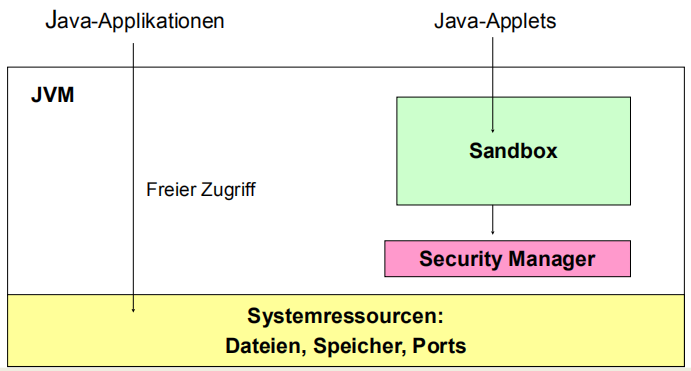
\includegraphics[width=0.85\linewidth]{Pics/JDKSandbox.PNG}
\end{figure}

\subsection{Sandboxing in Android}

\begin{itemize}
    \item Android ist eine der wichtigsten Smartphone-Plattformen (neben IOS), Marktanteil: >80\%
    \item Linux- und Java-basierte Plattform, mit einigen Änderungen
    \item Apps können auf das Gerät geladen werden
    \begin{itemize}
        \item Aus Google Play
        \item Aus anderen Quellen
    \end{itemize}
    \item Erweitertes Applet-Konzept, mit den bekannten Risiken
    \item \textbf{Android-Sandbox:} u.a. Apps werden jeweils unter eigener Unix-User ID installiert
\end{itemize}

\subsubsection{Android Permissions}

\begin{itemize}
    \item Benutzer muss Berechtigungen bei der Installation freigeben (jedoch ab Android 6.0 zur Laufzeit)
    \item Typische vordefinierte Berechtigungen: INTERNET, LOCATION, RECEIVE\textunderscore SMS
    \item Problem:
    \begin{itemize}
        \item Benutzer muss Entscheidung fällen
        \item Deshalb: Berechtigung grob granular (z.B. INTERNET)
    \end{itemize}
\end{itemize}

\subsubsection{Runtime-Bestätigung ab Android 6.0}

\begin{figure}[h!]
    \centering
    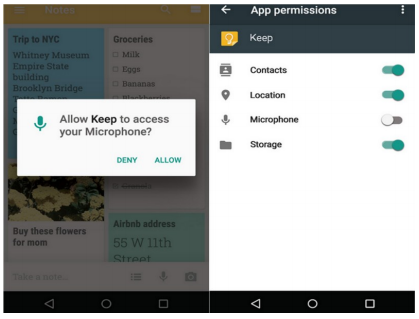
\includegraphics[width=0.6\linewidth]{Pics/AndroidPermission.PNG}
\end{figure}

\chapter{Kryptographie}

\textbf{Kryptographie = Kryptographie + Kryptoanalyse}

\begin{itemize}
    \item \textbf{Kryptographie:} Methoden zur Ver- und Entschlüsselung von Nachrichten und damit zusammenhängende Methoden
    \item \textbf{Kryptoanalyse:} Entschlüsselung ohne Zugriff auf den Schlüssel \\
    \item Kryptographie benötigt die Kryptoanalyse, und die erreichte Sicherheit der Verfahren beurteilen zu können
\end{itemize}

\section{Symmetrische Verschlüsselung}

\begin{figure}[h!]
    \centering
    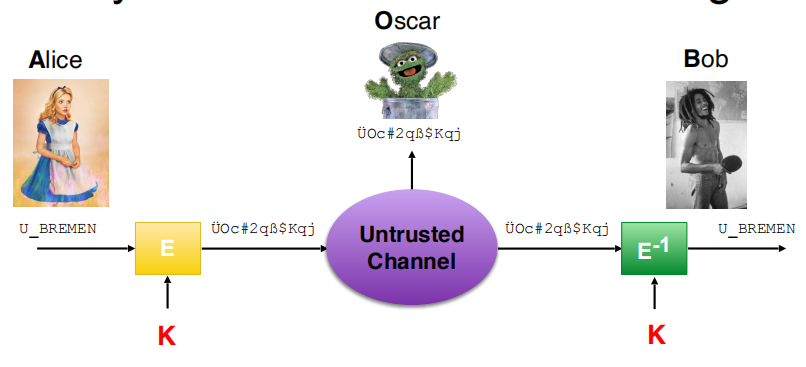
\includegraphics[width=0.85\linewidth]{Pics/Encryption.PNG}
\end{figure}

\newpage

\section{Terminologie}

\begin{itemize}
    \item Klartext (Plaintext): \textbf{P}
    \item Chiffretext/Geheimtext/Kryptotext (ciphertext): \textbf{C}
    \item Schlüssel (key): \textbf{K} \\
    \item Nachricht (message): \textbf{M}
    \begin{itemize}
        \item Wenn unwesentlich ist, ob verschlüsselt wird oder nicht
    \end{itemize}
\end{itemize}

\section{Kryptoanalyse: Angriffsklassen}

\begin{itemize}
    \item Ziel: \textbf{Schlüssel} finden ohne jene Information, die beim Ent- (oder Ver-)schlüsseln von neuem Text hilft
    \item Chiffretext-Angriff (\textbf{ciphertext-only attack}):
    \begin{itemize}
        \item Mehrere Chiffretexte stehen dem Angreifer zur Verfügung
        \item Nutzt statische Eigenschaften zwischen Chiffretexten aus; ggf. auch die des zugrunde liegenden Klartextes (sofern bekannt)
    \end{itemize} 
    \item Angriff mit bekanntem Klartext (\textbf{known-plaintext attack}):
    \begin{itemize}
        \item Sowohl Chiffretext/Klartextpaare stehen zur Verfügung
    \end{itemize}
    \item Angriff mit gewähltem Klartext (\textbf{chosen-plaintext attack}):
    \begin{itemize}
        \item Erzeuge eine Reihe von Klartexten
        \item Erhalte die dazugehörigen Chiffretexte
    \end{itemize}
    \item Angriff mit adaptiv gewähltem Klartext (oder Chiffretext) (\textbf{adaptive chosen-plaintext (or ciphertext) attack}):
    \begin{itemize}
        \item Führe verschiedene Angriffe mit gewähltem Klartext (Chiffretext) durch
        \item Nutze das Wissen der zuvor durchgeführten Angriffe zur Erzeugung von neuen Klartexten
    \end{itemize}
\end{itemize}

\newpage

\section{Historische Kryptographie}

* Heute zu leicht zu brechen

\subsection{Transposition}

\begin{itemize}
    \item Transposition: Verschieben von Buchstaben innerhalb des Textes
    \item Beispiel: Gartenzaun-Verschlüsselung
    \begin{figure}[h!]
        \centering
        
\includegraphics[width=0.6\textwidth]{Pics/Transposition.PNG}
    \end{figure}
    \item Problem: Verfahren muss geheim gehalten werden \\
    \item Skytale: Lederstreifen wurde um Holzstück \underline{bestimmte Größe} gewickelt und beschriftet
    \begin{figure}[h!]
        \centering
        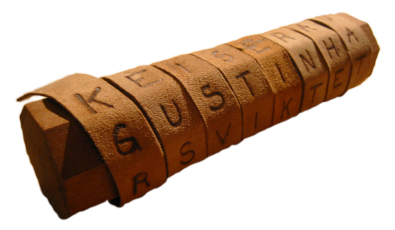
\includegraphics[width=0.6\textwidth]{Pics/Encryption2.PNG}
    \end{figure}
\end{itemize}

\subsection{Caesar-Chiffre}

\begin{itemize}
    \item Caesar-Chiffre: Jeder Buchstabe wird durch drittnächsten ersetzt (tim $\rightarrow$ wlp): $((x+3)\, \% \, 26)$
    \begin{figure}[h!]
        \centering
        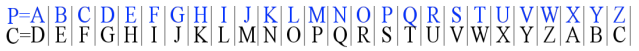
\includegraphics[width=0.85\textwidth]{Pics/CaesarCypher.PNG}
    \end{figure}
    \item Beispiel: PRUJHQ IUXHK
    \item Variante der Caesar-Chiffre: ROT13 $((x+3)\, \% \, 26)$
\end{itemize}

\subsection{Kerckhoffs-Prinzip}

\begin{itemize}
    \item Kerckhoffs-Prinzip: Kryptosystem bleibt sicher, wenn alles (auch das Verfahren) außer einem \textbf{Schlüssel} bekannt - Auguste Kerckhoffs, 1883
    \begin{itemize}
        \item Schlüssel kann leicht/oft getauscht werden
        \item Offenes kryptographisches Verfahren erlaubt externe Analyse \\
    \end{itemize}
    \item Erweiterte Caesar-Chiffre: Addend als Schlüssel
    \begin{itemize}
        \item Nur 25 (26-1) mögliche Schlüssel $\Rightarrow$ \textbf{brute force noch zu einfach}
    \end{itemize}
\end{itemize}

\subsection{Substitution}

\begin{itemize}
    \item Substitution: Ein Buchstabe wird durch einen anderen Buchstaben ausgetauscht
    \item Monoalphabetisch: Ein Buchstabe steht für genau einen anderen Buchstaben
    \item Problem wie bei der Caesar-Chiffre: Unwirksam, sobald Verfahren/Permutation bekannt ist
\end{itemize}

\subsubsection{Historie: Substitutionsschiffre}

Monoalphabetische Substitutionsschiffren

\begin{figure}[h!]
    \centering
    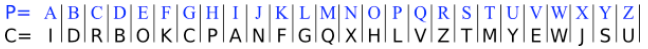
\includegraphics[width=0.85\textwidth]{Pics/Substitution.PNG}
\end{figure}

\begin{itemize}
    \item Schlüssel ist Permutation $K:A\leftrightarrow A$
    \begin{itemize}
        \item 21! > 3 $\times$ $10^26$ verschiedene Schlüssel
        \item Brute force ist bereits schwierig
    \end{itemize}
    \item Statistik-Angriff:
    \begin{itemize}
        \item Häufigste Buchstaben suchen (Detusch: E, N, I, S, R, A, ...)
        \item Nach häufigen Diagrammen/Trigrammen suchen
    \end{itemize}
\end{itemize}

\begin{figure}[h!]
    \centering
    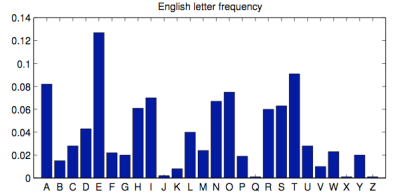
\includegraphics[width=0.41\textwidth]{Pics/Substitution2.PNG}
\end{figure}

\subsubsection{Polyalphabetische Chiffren}

\begin{figure}[h!]
    \centering
    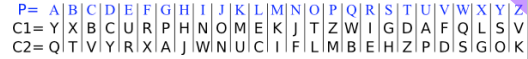
\includegraphics[width=0.75\textwidth]{Pics/PolyAlpha.PNG}
\end{figure}

\begin{itemize}
    \item ''Vigenère''-Chiffre:
    \begin{itemize}
        \item $K=k_0k_1k_2...k_{n-1}$
        \item $P=p_0p_1p_2...p_{m-1}$
        \item $c_i=(p_i+k_{(i\, \% \, n)})\, \% \, 26$ (via Codewort)
        \item Statt Modulo-Addition kann XOR oder jeder andere Gruppen-Operator verwendet werden
        \item Analyse: $n$ finden; Angriff auf Stellen mit gleichem $(i\, \% \, n)$
        \item Verallgemeinerung: Änderung der Substitutionsregel bei jedem Zeichen
    \end{itemize}
\end{itemize}

\begin{figure}[h!]
    \centering
    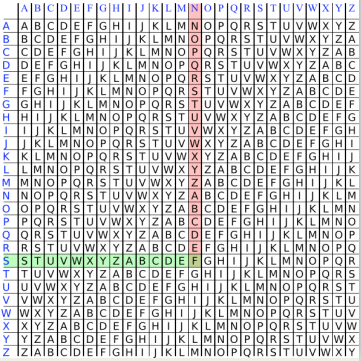
\includegraphics[width=0.6\textwidth]{Pics/PolyAlpha2.PNG}
\end{figure}

\section{Perfekte Chiffren}

\begin{itemize}
    \item Angreifer erhält keine Informationen aus dem Chiffretext
    \begin{itemize}
        \item Kenntnis eines Chiffretextes ändert nichts an der statischen Wahrscheinlichkeit möglicher Klartexte
    \end{itemize}
    \item Einzige Lösung: One-time-pad
    \begin{itemize}
        \item Schlüssel ist genauso lang wie Klartext und darf nur exakt einmal verwendet werden
        \item Bietet informationstheoretische Sicherheit
        \item $c_i=p_i\oplus k_i$ (XOR - jede andere Gruppe geht auch)
        \item Problem: Wie Schlüssel transportieren?
        \begin{itemize}
            \item Wiederverwendung ist \underline{extrem} gefährlich
        \end{itemize}
    \end{itemize}
\end{itemize}

\section{Blockchiffren: DES und AES}

\begin{itemize}
    \item Feste Blockgrößen und Schlüsselgrößen
    \begin{itemize}
        \item DES: 64 bit pro Block, 56 bit pro Schlüssel
        \item AES: 128 bit pro Block, 128, 196 oder 256 bit pro Schlüssel
    \end{itemize}
    \item Produktchiffre (rundenbasierte Algorithmen)
    \begin{itemize}
        \item DES: 16 Runden, AES (Rijndael): 10-14 Runden
    \end{itemize}
    \item DES gilt als unsicher, 3DES = $E_{K1}(D_{K2}(E_{K3}(P)))$ (168 bit)
    \item AES wurde als Nachfolger von DES entwickelt
    \begin{itemize}
        \item Offenes Auswahlverfahren
        \item Viele Kryptoanalyse-Versuche vor und nach der Auswahl
    \end{itemize}
\end{itemize}

\subsection{Nutzung von Blockchiffren: Modes of Operation (Betriebsarten)}

\begin{itemize}
    \item \textbf{ECB} (Electronic Codebook): Je n Bit des Klartextes werden einzeln für sich verschlüsselt.
    \item Problem: Identitäten/Redundanzen im Klartext werden im Chiffretext sichtbar
    \begin{itemize}
        \item Kryptanalyst kann sich mit known-plaintext ''Bausteine'' schaffen
        \item Wiederholte Nachrichten sind leicht zu erkennen
    \end{itemize}
\end{itemize}

\newpage

\section{Funktionsweise: ECB}

\begin{itemize}
    \item Je n Bits des Klartextes (=Block) werden einzeln für sich verschlüsselt
    \begin{figure}[h!]
        \centering
        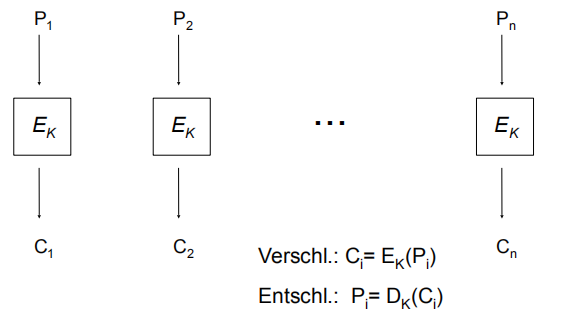
\includegraphics[width=0.75\linewidth]{Pics/ECB.PNG}
    \end{figure}
\end{itemize}

\subsubsection{ECB: Visualisierung}

\begin{figure}[h!]
    \centering
    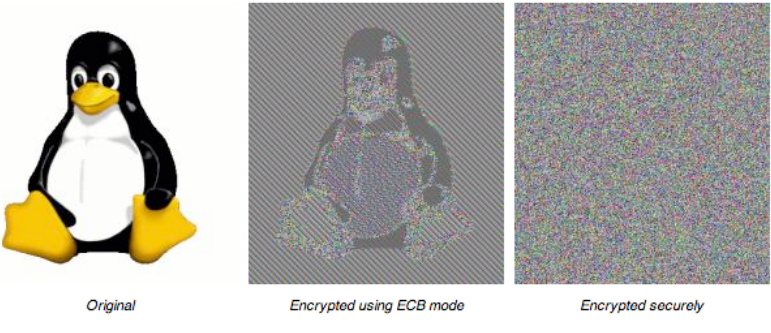
\includegraphics[width=0.75\linewidth]{Pics/ECB2.PNG}
\end{figure}

\section{CBC: Cipherblock Chaining}

\begin{itemize}
    \item Vor der Verschlüsselung wird $P_i$ mit $C_{i-1}$ verändert (XOR)
    \item Zum Schutz von $P_1$ wird zu Beginn eine Zufallszahl vorgegeben (Initialisation Vector, IV)
    \item Bitfehler zerstört aktuellen Block und führt zu Bitfehler im Folgeblock
\end{itemize}

\newpage

\subsubsection{Funktionsweise: CBC}

\begin{figure}[h!]
    \centering
    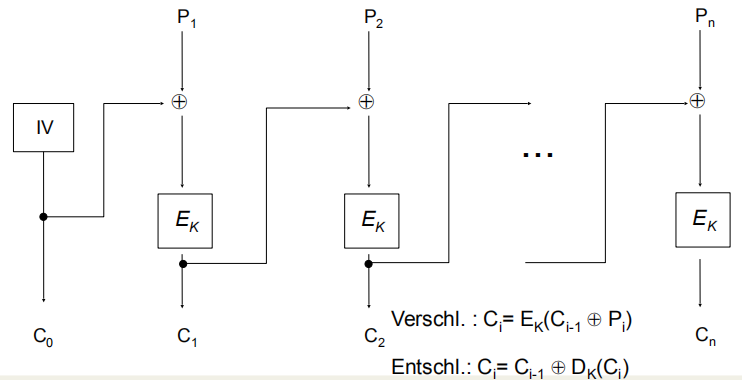
\includegraphics[width=0.75\linewidth]{Pics/CBC.PNG}
\end{figure}

\section{Padding}

\begin{itemize}
    \item Input ist nicht immer genau n Blöcke groß
    \item Auffüllen mit \textbf{Padding}
    \item Wie wieder entfernen?
    \item $\rightarrow$ Immer Padding,
    \begin{itemize}
        \item z.B.: letztes Byte sagt die Anzahl der Bytes (SSLv3)
        \item Besser: PKCS \#7: Alle Padding-Bytes mit dem selben Wert
    \end{itemize}
    \begin{figure}[h!]
        \centering
        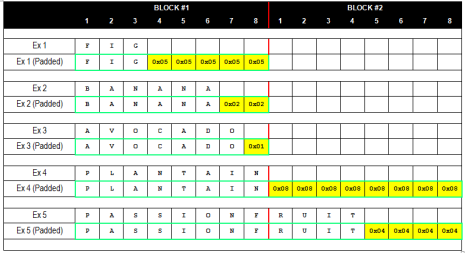
\includegraphics[width=0.85\linewidth]{Pics/Padding.PNG}
    \end{figure} 
\end{itemize}

\section{Weitere Stromchiffren-Modi}

\begin{itemize}
    \item \textbf{CTR} (Counter Mode): \\ $R_i = E_K(i+O)$, $C_i=P_i\oplus R_i$
    \item Offset O wird wie IV mit Chiffretext übertragen
    \item Vorteil: Direktzugriff in die Mitte des Stroms \\
    \item \textbf{CFB} (Cipher Feedback Mode): \\ $R_i = E_K(C_{i-1})$, $C_i = P_i\oplus R_i$
    \begin{itemize}
        \item Ein Bitfehler im Chiffretext erzeugt einen Bitfehler und zerstört den Folgeblock
    \end{itemize}
    \item $C_0$ wird als IV mit Chiffretext übertragen
\end{itemize}

\subsection{Funktionsweise: CTR}

\begin{figure}[h!]
    \centering
    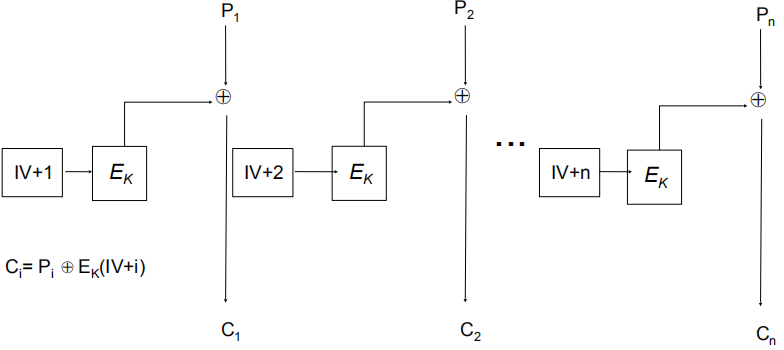
\includegraphics[width=0.85\linewidth]{Pics/CTR.PNG}
\end{figure} 

\subsection{Angriffe gegen Stromchiffren}

\begin{itemize}
    \item Modifizierte Wiedereinspielung (vor allem OFB/CTR)
    \begin{itemize}
        \item Ist Struktur bekannt, reicht eventuell ein ''Bitfehler''
        \item Schutz: Integritätsprüfung 
    \end{itemize}
    \item Bei Wiederverwendung der IV/K-Kombination:
    \begin{itemize}
        \item $E(A)\oplus E(B)=(A\oplus R)\oplus (B\oplus R) = A\oplus B$
        \item Schutz: K oft genug wechseln (und IV nie wiederholen)
    \end{itemize}
\end{itemize}

\newpage

\section{Schlüsselerzeugung}

\subsection{Qualität von Zufallszahlen}

\begin{figure}[h!]
    \centering
    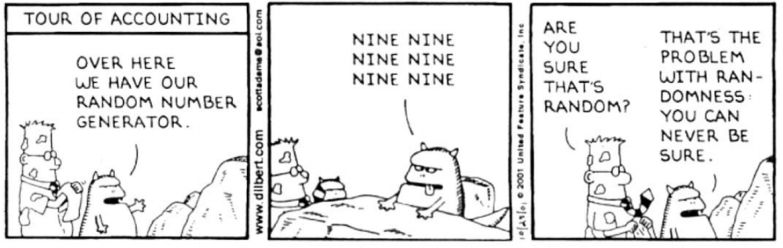
\includegraphics[width=\linewidth]{Pics/Random1.PNG}
\end{figure} 

\subsection{Entropie}

\begin{itemize}
    \item Entropie in der Informationstheorie (Shannon 1948): Informationsgehalt \\ ''Maß der Unsicherheit'' (Überraschung)
    \item N völlog zufällige Bits $\rightarrow$ Entropie N bit
    \item Werden Bits vorhergesagt, sinkt die Entropie Redundanzen \\ Statische Regelmäßigkeit
    \item Verlustlose Kompression kann auf Entropie, aber nicht weiter komprimieren
\end{itemize}

\subsection{Zufallszahlen}

\begin{itemize}
    \item Wichtig für Sitzungsschlüssel etc.
    \begin{itemize}
        \item Viele Angriffe basieren auf der Möglichkeit, Zufallszahlen zu raten
    \end{itemize}
    \item True RNG: Entropie wächst mit jedem Bit
    \item Pseudo-RNG, Deterministischer RNG: Entropie steckt im ''Seed'' (Startwert), dann konstant
    \begin{itemize}
        \item Hybridformen: kontinuierliches Seeding
    \end{itemize}
    \item Wie generieren?
    \begin{itemize}
        \item Physikalische Prozesse und Entropiequellen
        \begin{itemize}
            \item Thermisches Rauschen, Jitter, Metastabile Prozesse, radioaktive Zerfallsprozesse
        \end{itemize}
        \item Befehlsweise zu verwenden
        \begin{itemize}
            \item Computerhardware (Festplatten, Sound- und Videokarten)
            \item Benutzereingaben
        \end{itemize}
    \end{itemize}
    \item Nachteile von Hardware für Zufallszahlen:
    \begin{itemize}
        \item Oft langsam
        \item Nicht immer verfügbar
        \item Ohne Software-Hilfe sehr aufwendig
    \end{itemize}
    \item Linux Entropiepool
    \begin{itemize}
        \item Benutzer: Tastatur, Maus
        \item Hardware: Netzlast, Interrupts
    \end{itemize} Linux: \textbackslash dev\textbackslash random \\ Aber: immernoch sehr langsam!
    \item \textbackslash dev\textbackslash urandom:
    \begin{itemize}
        \item Nimmt Daten aus Entropie-Pool
        \item Blockiert nicht auf leerem Pool
        \item Erzeugt dann selbst Zufallszahlen via DRNG (Deterministic Random Number Generator)
    \end{itemize}
    \item Pseudozufallszahlengenerator (Pseudo Random Number Generator PRNG)
    \begin{itemize}
        \item Erzeugt aus einem Initialisierungswert (seed) immer gleiche Folge von Zufallszahlen
    \end{itemize}
\end{itemize}

\subsection{Block-Chiffre als Pseudo-Zufallszahlengenerator}

\begin{itemize}
    \item Kryptographisch starker PRNG: $R_i=E_K(R_{i-1})$
    \item \textbf{OFM} (Output Feedback Mode): \\ $C_i=P_i\oplus R_i$ (mit $R_i=E_K(R_{i-1})$)
    \item \textbf{Achtung:} Wiederverwendung von $K/R_0=$ Bombe
\end{itemize}

\newpage

\section{Hash-Funktionen}

\subsection{Kryptographischer Hash}

\begin{itemize}
    \item Hash dampft variabel lange Binärdaten in Fingerabdruck ein:
    \begin{figure}[h!]
        \centering
        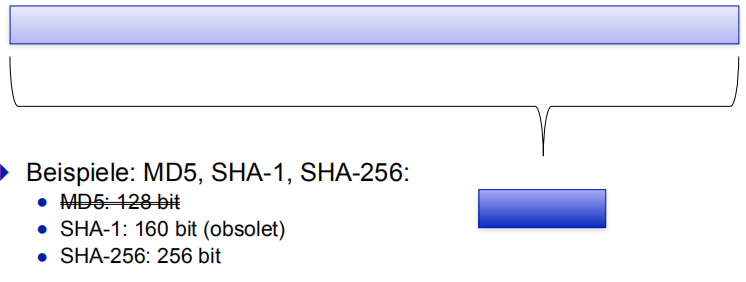
\includegraphics[width=\linewidth]{Pics/Hashing1.PNG}
    \end{figure} 
\end{itemize}

\subsubsection{Was ist ein guter Kryptographischer Hash?}

\begin{itemize}
    \item Schwierig zu erreichendes Ziel:
    \begin{itemize}
        \item Kollisionsresistent: schwer, $x\neq y$ zu finden mit $h(x)=h(y)$
        \begin{itemize}
            \item Zwei Personen finden, die am gleichen Tag Geburtstag haben
        \end{itemize}
    \end{itemize}
    \item Etwas weniger problematisch in der Sicherheitsbetrachtung:
    \begin{itemize}
        \item Urbildresistent: schwer, zu einem a ein y zu finden mit $a=h(y)$
        \begin{itemize}
            \item Zu einem gegebenen Geburtstagsdatum die passende Person finden
        \end{itemize}
        \item Urbild-2: schwer, zu einem x ein $y\neq x$ zu finden mit $h(x)=h(y)$
        \begin{itemize}
            \item Eine zweite Person finden, die am gleichen Tag Geburtstag hat
        \end{itemize}
    \end{itemize}
\end{itemize}

\subsection{Geburtstagsparadoxon}

\begin{itemize}
    \item 23 Personen sitzen in einem Raum
    \item Wie hoch ist die Wahrscheinlichkeit, dass eine dieser Personen am selben Tag wie ich Geburtstag hat?
    \item Wie hoch ist die Wahrscheinlichkeit, dass zwei von diesen Personen am selben Tag Geburtstag haben?
\end{itemize}

\begin{itemize}
    \item Mit 6.1\% Wahrscheinlichkeit hat eine Person von 23 am selben Tag Geburtstag
    \item Von 23 Personen haben mit 50\% Wahrscheinlichkeit zwei am selben Tag Geburtstag
    \item $n\, x(n-1)/2$ Verbindungen
    \item Allgemein: aus k möglichen Werten reichen $k^\frac{1}{2}$ für ca. 50\% Kollisionswahrscheinlichkeit
\end{itemize}

\begin{figure}[h!]
    \centering
    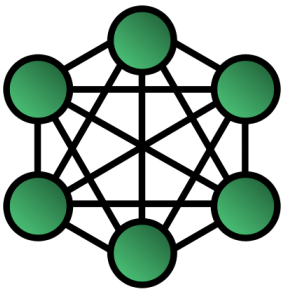
\includegraphics[width=0.25\linewidth]{Pics/Hashing2.PNG}
\end{figure} 

\subsubsection{Einfluss auf das Geburtstagsparadoxons}

\begin{itemize}
    \item Erinnerung: Von 23 Personen haben mit 50\% Wahrscheinlichkeit zwei am selben Tag Geburtstag
    \begin{itemize}
        \item Allgemein: aus k möglichen Werten reichen $k^\frac{1}{2}$ für ca. 50\% Kollisionswahrscheinlichkeit
    \end{itemize}
    \item SHA-1: $2^160$ Möglichkeiten
    \begin{itemize}
        \item $2^80$ Versuche ergeben mit $p\geq 0.5$ Kollision (''Geburtstagsangriff'')
    \end{itemize}
    \item Neue Angriffe auf SHA-1 reduzieren $2^80$ auf $2^63$
    \begin{itemize}
        \item Immernoch ähnlich $2^64$ (MD5 vor den Angriffen)
        \item Übergang auf SHA-2 (SHA-256, SHA-512, ...)
    \end{itemize}
\end{itemize}

\newpage

\subsection{Wir bauen uns einen Hash: Merkle-Damgård}

\begin{figure}[h!]
    \centering
    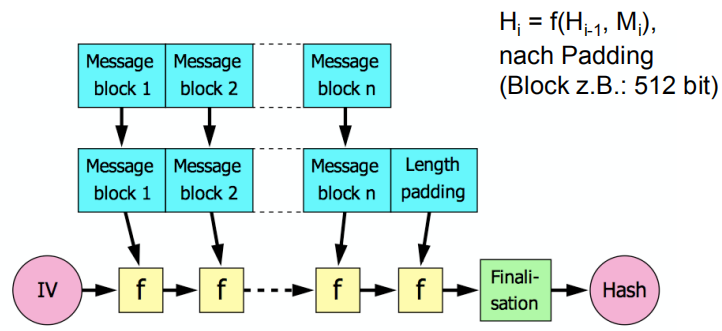
\includegraphics[width=\linewidth]{Pics/Hashing3.PNG}
\end{figure} 

\subsection{Padding: Auffüllen auf Blockgröße}

\begin{figure}[h!]
    \centering
    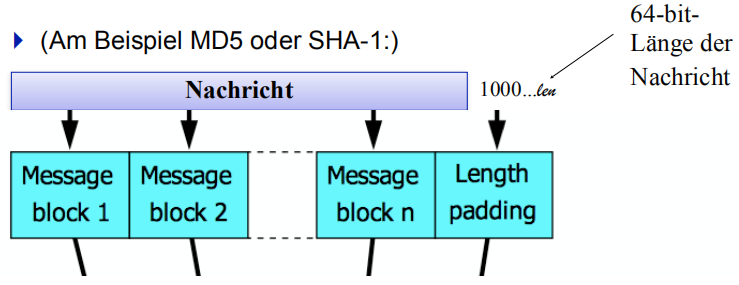
\includegraphics[width=\linewidth]{Pics/Padding2.PNG}
\end{figure} 

\newpage

\begin{figure}[h!]
    \centering
    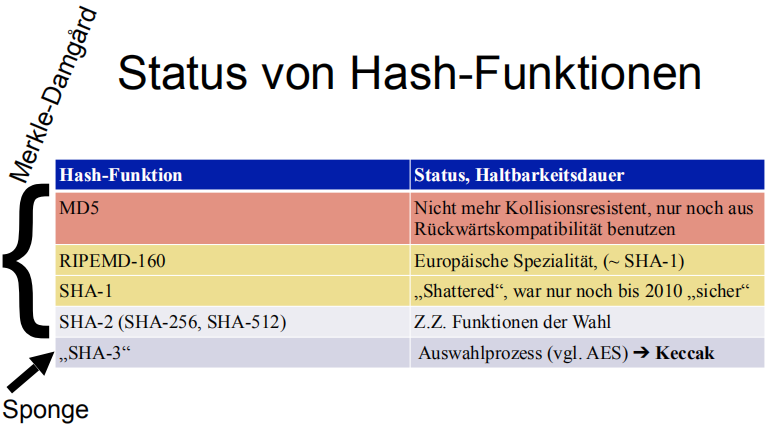
\includegraphics[width=\linewidth]{Pics/Hashing4.PNG}
\end{figure} 

\begin{figure}[h!]
    \centering
    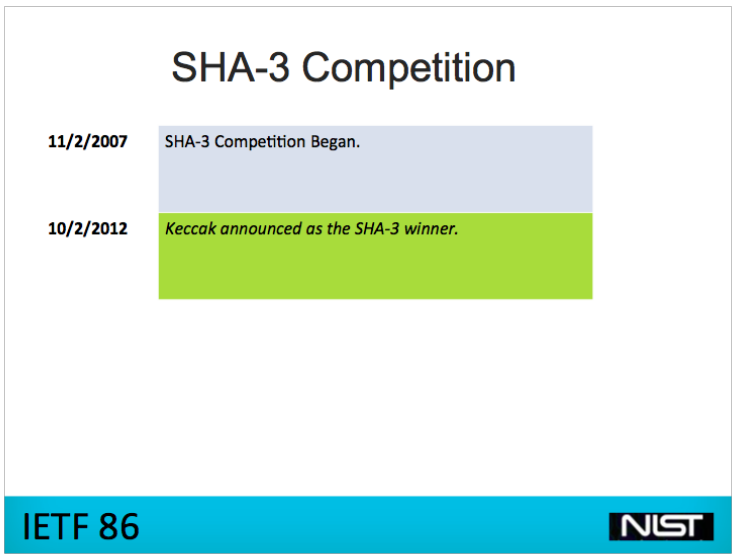
\includegraphics[width=\linewidth]{Pics/Hashing5.PNG}
\end{figure} 

\newpage

\begin{figure}[h!]
    \centering
    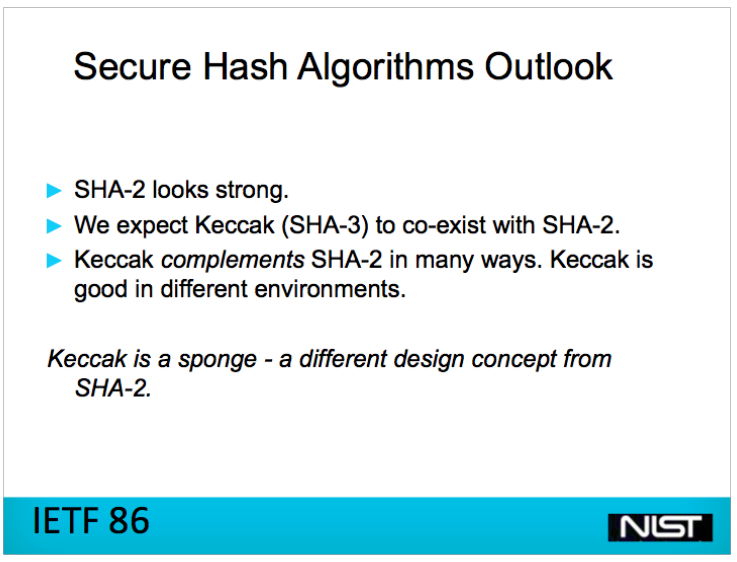
\includegraphics[width=0.9\linewidth]{Pics/Hashing6.PNG}
\end{figure}

\begin{figure}[h!]
    \centering
    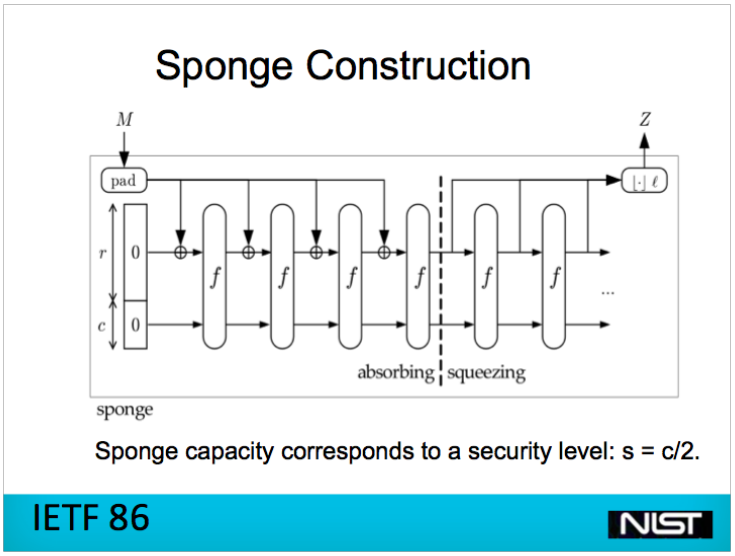
\includegraphics[width=0.9\linewidth]{Pics/Hashing7.PNG}
\end{figure} 

\newpage

\begin{figure}[h!]
    \centering
    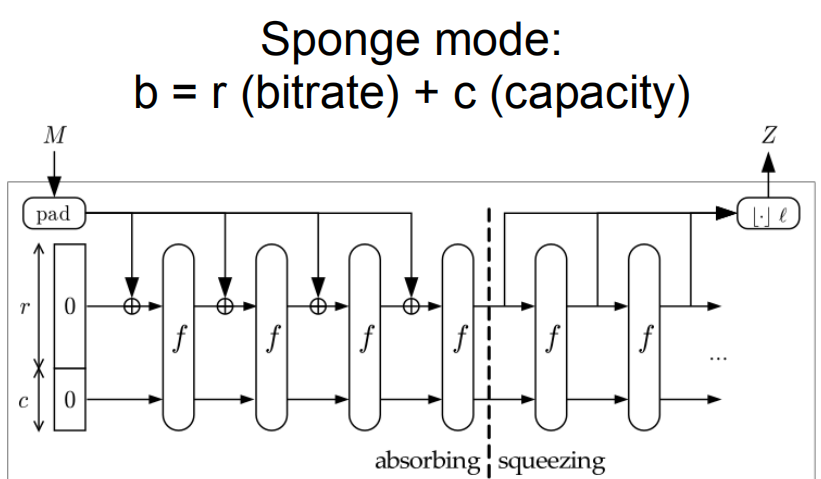
\includegraphics[width=\linewidth]{Pics/Hashing8.PNG}
\end{figure} 

\section{Message Authentication Codes (MAC)}

\begin{itemize}
    \item Nicht jede Nachricht möchte man signieren (aufwendig)
    \item Idee:
    \begin{itemize}
        \item Erst gemeinsames Geheimnis vereinbaren
        \item Sender verbindet dieses dann mit Nachricht kryptographisch
        \item Empfänger wendet die gleiche Funktion an
        \item Nachricht muss echt sein, wenn Ergebnis übereinstimmt
    \end{itemize}
    \item ''Hash mit Schlüssel'' / Blockchiffren zur Nachrichtenauthentisierung
\end{itemize}

\subsection{Einsatz von Hash-Funktionen für MACs: HMAC}

\begin{figure}[h!]
    \centering
    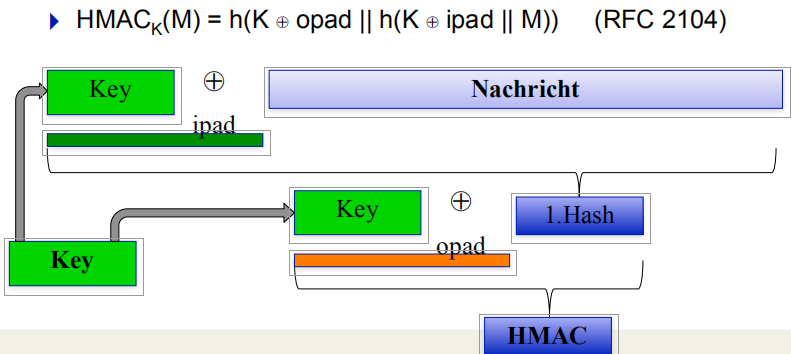
\includegraphics[width=0.75\linewidth]{Pics/Hashing9.PNG}
\end{figure} 

\newpage

\subsection{Exkurs: CBC-MAC (Message Authentication Code)}

\begin{itemize}
    \item Integrität: Hash über Nachricht
    \item Kann nur mit Schlüssel K erstellt oder verifiziert werden
\end{itemize}

\begin{figure}[h!]
    \centering
    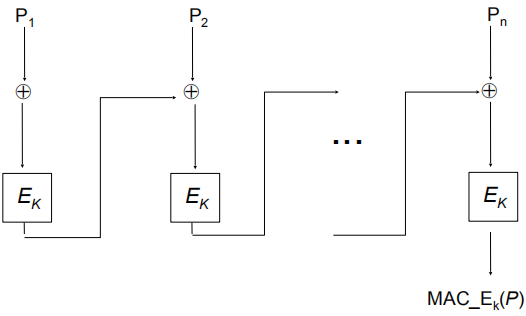
\includegraphics[width=0.75\linewidth]{Pics/CBC-MAC.PNG}
\end{figure} 

\subsection{Kombination MAC/Verschlüsselung}

\begin{itemize}
    \item Stromchiffre braucht immer Integritätsprüfung
    \item Kombination möglich?
    \item OCB: Offset Codebook
    \begin{itemize}
        \item Literatur:
        \begin{itemize}
            \item Rogaway, Bellare, Black, Krovetz: OCB: A Block-Cipher Mode of Operation for Efficient Authenticated Encryption
        \end{itemize}
    \end{itemize}
    \item Problem: Patentiert
    \item 802.11i verwendet stattdessen CTR + CBC-MAC
    \begin{itemize}
        \item Details: RFC 3610 
    \end{itemize}
\end{itemize}

\subsection{Authenticated Encryption with Associated Data (AEAD)}

\subsubsection{Authenticated Encryption}

\begin{itemize}
    \item Vertraulichkeit + Integrität + Authentizität
    \item effizient mit Block-Verschlüsselung realisierbar \\ $\rightarrow$ benötigt Counter und CBC-MAC
\end{itemize}

\subsubsection{Mechanismus: RFC 5116}

\begin{itemize}
    \item Verschlüsselung: $K\times N\times P\times A \rightarrow A\times C$
    \item Entschlüsselung: $K\times N\times A\times C \rightarrow A\times P$
    \item AHEAD-Algorithmus legt Länge von K,K\textunderscore LEN, fest \\ K - Key, A Associated Data, P - Plaintext, N - Nonce, C - Cyphertext
\end{itemize}

\section{Wie sicher ist mein Kryptosystem?}

\begin{itemize}
    \item Aussage: man müsste zum Brechen den gleichen Aufwand treiben wie für einen Brute-Force-Angriff mit $2^n$ Schritten
    \item n ist die Sicherheitsstufe in ''Bits''
    \item z.B. AES-128: ungebrochen, also bräuchte man $2^128$ Schritte für einen Brute-Force-Angriff
    \begin{itemize}
        \item ''128-Bit-Sicherheit''
    \end{itemize}
    \item Bei anderen Verfahren ist der Zusammenhang nicht immer so einfach!
\end{itemize}

\subsection{Levels of Security}

\begin{figure}[h!]
    \centering
    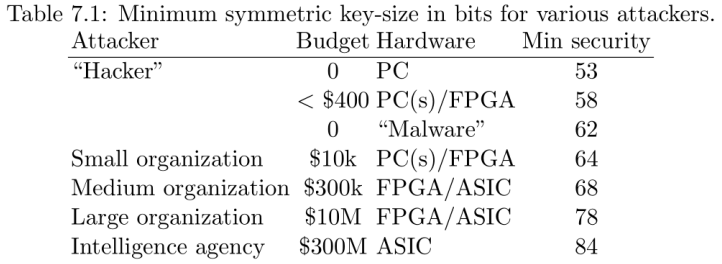
\includegraphics[width=\linewidth]{Pics/SecurityLevel1.PNG}
\end{figure} 

\newpage

\begin{figure}[h!]
    \centering
    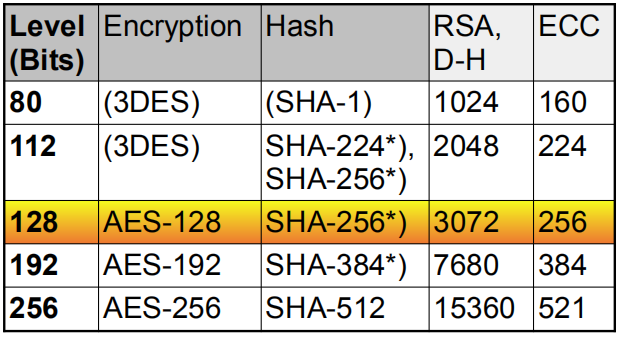
\includegraphics[width=\linewidth]{Pics/SecurityLevel2.PNG}
\end{figure} 

\newpage

\section{Asymmetrische Kryptographie}

\textbf{Das Problem mit der symmetrischen Verschlüsselung}

\begin{itemize}
    \item Die beiden Kommunikationspartner Alice und Bob brauchen ein \textbf{gemeinsames Geheimnis $K_{AB}$}
\end{itemize}

\begin{figure}[h!]
    \centering
    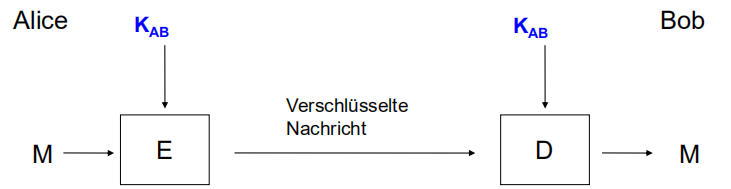
\includegraphics[width=\linewidth]{Pics/SymmetricEncryption.PNG}
\end{figure} 

\subsection{Schlüsselverteilungsproblem}

\begin{itemize}
    \item Wie Schlüssel $K_{AB}$ etablieren, wenn man sich noch nicht kennt?
    \begin{itemize}
        \item Symmetrische Verschlüsselung setzt einen vertraulichen Informationskanal zur Übertragung des Schlüssels $K_{AB}$ voraus! \\ (Problem des Schlüsselsaustauschs bzw. Schlüsselsvereinbarung)
    \end{itemize}
    \item Wie viele Schlüssel braucht man für 2, 3, 4, 10, 1000 Teilnehmer, wenn jeder jedem Nachrichten schicken können soll, die kein anderer lesen kann?
    \begin{itemize}
        \item Für 2, 3, 4, 10, 10, 1000 Teilnehmer werden 1, 3, 6, 45, 499500 Schlüssel benötigt.
    \end{itemize} 
    \item Allgemein: Bei n potentiellen Kommunikationsteilnehmern benötigt man bis zu $n^x(n-1)/2$ Schlüssel.
    \item n = 10000 entspricht ungefähr 50000000 Schlüsseln!
\end{itemize}

\section{Asymmetrische (Public Key-) Verschlüsselung}

\begin{itemize}
    \item Whitfield Diffie, Martin E. Hellman (1976): Warum müssen eigentlich Sender und Empfänger denselben Schlüssel benutzen?
    \item Ein Schlüsselpaar ($K_E$,$K_D$) pro Kommunikationspartner
    \item Ein \textbf{öffentlicher} und ein \textbf{privater} Schlüssel
    \item Ein Schlüssel zum Verschlüsseln ($K_E$), der andere zum Entschlüsseln ($K_D$)
\end{itemize}

\newpage

\begin{figure}[h!]
    \centering
    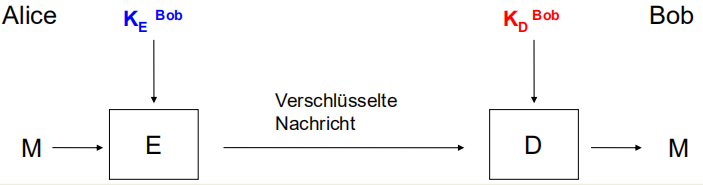
\includegraphics[width=\linewidth]{Pics/SymmetricEncryption2.PNG}
\end{figure} 

\subsection{Allgemeine Eigenschaften asymmetrischer Verfahren}

\begin{itemize}
    \item $K_E$ sei der \textbf{öffentliche}, $K_D$ der \textbf{private} Schlüssel
    \item Die Schlüsselpaare ($K_E$,$K_D$) müssen folgende Eigenschaft erfüllen:\\ Für alle Nachrichten M: D (E (M, $K_E$), $K_D$) = M \\ (Eine Nachricht, die mit $K_E$ verschlüsselt wird, wird mit $K_D$ entschlüsselt und umgekehrt)
    \item Solche Schlüsselpaare müssen \textbf{leicht zu erzeugen} sein.
    \item Ver- und Entschlüsselung (E und D) sind \textbf{effizient durchführbar}
    \item $K_D$ ist aus $K_E$ \textbf{nicht} mit \textbf{vertretbarem Aufwand berechenbar}
\end{itemize}

\subsection{Beispiele für asymmetrische Verfahren}

\begin{itemize}
    \item RSA (''Quasi-Standard'')
    \item ElGamal-Verfahren
    \item Schlüsselvereinbarung nach Diffie und Hellman
\end{itemize}

\section{Einweig-Funktionen}

\begin{itemize}
    \item \textbf{Basis} für asymmetrische Kryptographie sind Einweg-Funktionen (\textbf{one-way}) \\ $f:X\rightarrow Y$ \\ \textbf{Eigenschaften von Einweig-Funktionen:} \\ 1) $\forall x\in X$ gilt: $f(x)$ ist \textbf{effizient} berechenbar; und \\ 2) für fast alle $y\in Y$ gilt, dass es \textbf{nicht effizient} möglich ist, das Urbild zu y zu berechnen, also $x\in X$, mit $y=f(x)$
    \item Bis heute nicht bewiesen, ob überhaupt Einwegfunktionen existieren.
    \item Bewiesen ist: Sie existieren gdw. $P\neq NP$.
\end{itemize}

\newpage

\begin{figure}[h!]
    \centering
    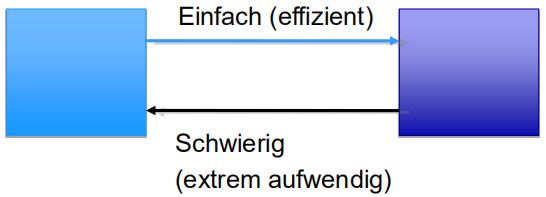
\includegraphics[width=0.85\linewidth]{Pics/OneWayFunction.PNG}
\end{figure} 

\begin{itemize}
    \item ''Extrem aufwendig'' = nicht in der Lebenszeit des Universums zu schaffen (''unmöglich'')
\end{itemize}

\subsection{Einweg-Funktionen mit Falltür}

\begin{itemize}
    \item Einweg-Funktionen \textbf{mit Falltür} (\textbf{trapdoor one-way}):
    \begin{itemize}
        \item mit Zusatzinformation sind Urbilder effizient berechenbar
    \end{itemize}
    \item Gute Kandidaten für Einweg-Funktionen mit Falltür:
    \begin{itemize}
        \item 1) \textbf{Potenzfunktion modulo n} mit n=pq, p und q Primzahlen $f:x\rightarrow x^e$ mod n
        \item 2) \textbf{Exponentialfunktion modulo p}, p Primzahl $f:x\rightarrow g^x$ mod p
    \end{itemize}
    \item Jetzt: Umkehrung der Exponentialfunktion
\end{itemize}

\subsection{Primitivwurzel}

\begin{itemize}
    \item Vorausgesetzte Begrifflichkeit: \\ Gegeben p Primzahl. Eine \textbf{Primwurzel g} mod p erzeugt alle von 0 verschiedenen Reste mod p (Generator).
\end{itemize}

\begin{figure}[h!]
    \centering
    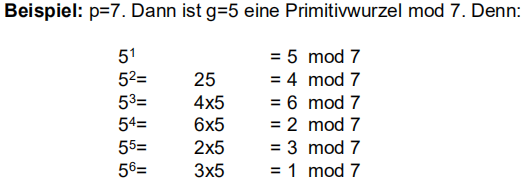
\includegraphics[width=0.85\linewidth]{Pics/PrimitiveRoot.PNG}
\end{figure} 

\subsection{Problem des diskreten Logarithmus /1}

\begin{itemize}
    \item Gegeben p Primzahl, $g\leq p-1$ primitive Wurzel und ganze Zahl y. \\ Bestimme die eindeutige Zahl k ($q\leq k \leq p-1$) so, dass $y=g^x$ mod p
    \item Bezeichnung für k: d$\log_g y$, z.B.: d$\log_5 4 = 2$
    \item \textbf{Ganzzahliges} Problem (''diskret'')
    \item Diskreter Logarithmus als \textbf{Umkehrung} der diskreten Exponentialfunktion
\end{itemize}

\subsection{Problem des diskreten Logarithmus /2}

\begin{itemize}
    \item Berechnung der Exponentialfunktion (auch für große p) effizient durchführbar
    \item Bestimmung des diskreten Logarithmus aber nicht
    \begin{itemize}
        \item Nur Inspektion (alles durchprobieren)
        \item Problem aus NP
    \end{itemize}
    \item $f:x\rightarrow g^x$ mod p ist eine Einweg-Funktion mit Falltür (x)
\end{itemize}

\begin{figure}[h!]
    \centering
    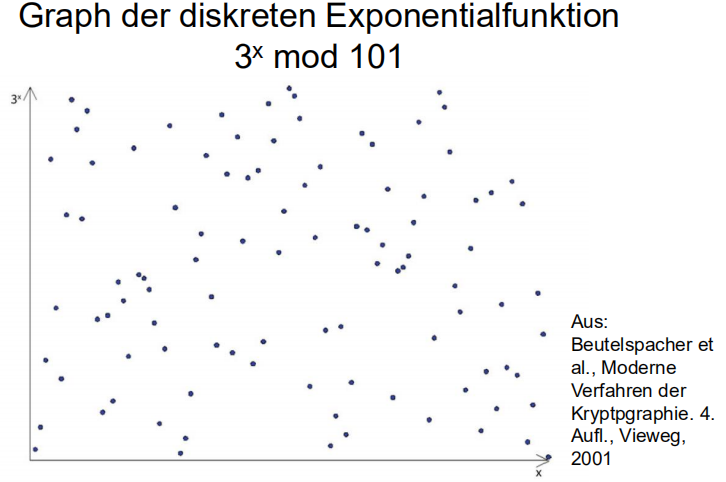
\includegraphics[width=0.85\linewidth]{Pics/DiscreetLogarithmGraph.PNG}
\end{figure} 

\newpage

\section{Schlüsselvereinbarung nach Diffie und Hellman}

\begin{itemize}
    \item \textbf{Ziel:} Vereinbarung eines gemeinsamen geheimen Schlüssels, \textbf{ohne diesen über die Leitung zu schicken} (z.B. für eine symmetrische Verschlüsselung)
    \item \textbf{Achtung:} Diffie-Hellman allein liefert keine Verschlüsselung, keine Authentisierung der Partner!
    \begin{itemize}
        \item Einsatz u.a. in TLS, Kerberos, IPsec-Protokollen, PGP, S/MIME
        \item Basiert auf dem Problem des diskreten Logarithmus
    \end{itemize}
    \item Funktionsweise: 
    \begin{itemize}
        \item Wähle große \textbf{Primzahl p} (allen Teilnehmern bekannt)
        \item Wähle einen allen Teilnehmern bekannten \textbf{Wert g}, der primitive Wurzel von p ist \\ Es gilt also: $\{ g^1,...,g^{p-2},g^{p-1}\} = \{ 1,2,...,p-2,p-1\}$.
        \item g, p öffentlich bekannt
    \end{itemize}
\end{itemize}

\begin{figure}[h!]
    \centering
    \includegraphics[width=\linewidth]{Pics/DiffieHellman.PNG}
\end{figure} 

\section{ElGamal-Verschlüsselungsverfahren}

\begin{itemize}
    \item Taher ElGamal, 1985
    \item Public-Key-Verfahren, basiert auch auf dem diskreten Logarithmus
    \item Variante von Diffie-Hellman, ähmliche Idee
    \item Wir setzen also wieder voraus: p Primzahl, g Primitivwurzel
\end{itemize}

\subsection{Funktionsweise: ElGamal-Verschlüsselung}

\begin{itemize}
    \item \textbf{Schlüsselerzeugung} von Bob:
    \begin{itemize}
        \item Wählt zufällig eine Zahl $b$ und berechnet $\beta := g^b \, mod \, p$
        \item Veröffentlicht ($\beta ,g,p$) als \textbf{öffentlichen Schlüssel}
        \item $b$ ist der \textbf{private Schlüssel}
    \end{itemize}
    \item \textbf{Verschlüsselung} einer Nachricht M (mit M < p):
    \begin{itemize}
        \item Alice schlägt $(\beta ,g,p)$ im Schlüsselverzeichnis nach.
        \item Alive wählt eine \textit{Nonce} (einmalige Zufallszahl) $a$ und berechnet: \\ $\alpha := g^a \, mod \, p$ \\ $k:=\beta ^a \, mod \, p$ \\ $c:=kM \, mod \, p$ (Maskierung der Nachricht M mit k)
    \end{itemize}
    \item Versenden der Nachricht: Alice verschickt die chiffrierte Nachricht $(\alpha , c)$ an Bob
    \begin{itemize}
        \item \textbf{Der Chfifretext ist doppelt so lang wie der Klartext!}
    \end{itemize}
    \item \textbf{Entschlüsselung:}
    \begin{itemize}
        \item 1) Bob berechnet zunächst wieder k:  $$a^b \, mod \, p = (g^a)^b \, mod \, p = g^{ab}\, mod\, p = g^{ba}\, mod\, p = (g^b)^a\, mod \, p$$ $$=\beta ^a \, mod\, p = k$$
        \item 2) Mittels k kann Bob dann wieder die Nachricht M berechnen: $$k^{-1}c\, mod\, p= k^{-1}kM\, mod\, p = M\, mod \, p  = M$$
    \end{itemize}
\end{itemize}

\section{Asymmetrische Kryptographie auf Basis elliptischer Kurven}

\begin{itemize}
    \item Elliptic Curve Cryptography (ECC), Miller 1985, Koblitz 1987
    \item Verwendet elliptische Kurven (über Körper K) als algebraische Struktur
    \begin{itemize}
        \item Zyklische Gruppe (Erzeugt aus primitivem Element)
        \item Spezielle Addition auf dieser Gruppe
        \item Beispiel: Elemente der Gruppe sind Punkte (x,y) mit der Eigenschaft $y^2=x^3+ax+b$ 
    \end{itemize}
\end{itemize}

\newpage

\begin{figure}[h!]
    \centering
    \includegraphics[width=0.5\linewidth]{Pics/ECC.PNG}
\end{figure} 

\subsection{Praktische Bedeutung von ECC}

\begin{itemize}
    \item Problem des diskreten Logarithmus auch auf EC übertragbar
    \item Implementierung von Diffie-Hellman (ECDH) und ElGamal auf Basis von ECC
    \item Kleinere Schlüssellängen
    \begin{itemize}
        \item 160 (224) Bit entspricht 1024 (2048) Bit bei herkömmlicher asymmetrischer Kryptographie
        \item Weniger Speicherbedarf und Rechenleistung
        \item Deshalb auch Einsatz auf Chipkarten
    \end{itemize}
    \item Implementierungen in den meisten aktuellen Krypto-Bibliotheken vorhanden wie z.B. OpenSSL, Bouncycastle, Java
\end{itemize}

\section{RSA-Algorithmus}

\begin{itemize}
    \item \textbf{RSA (1977/1978):} Ron Rivest, Adi Shamir, Len Adleman
    \begin{itemize}
        \item 1983 patentiert, seit 2000 frei
        \item Ähnliches System bereits 1973 von Clifford Cocks erfunden, aber geheim gehalten
    \end{itemize}
    \item \textbf{Einsatzbereiche:} Verschlüsseln, Signieren, Schlüsselaustausch
    \item \textbf{Basis:} Primfaktorzerlegung
\end{itemize}

\subsection{RSA: Funktionsweise}

\begin{itemize}
    \item Hier: nur skizziert; detaillierte Beschreibung in der Literatur
    \begin{itemize}
        \item 1) Wähle Primzahlen p, q, \textbf{Modul n} = pq
        \item 2) Wähle $d$ so, dass ggT((p-1)(q-1),d)=1,
        \item 3) Berechne $e$ mit $ed=1$ mod ((p-1)(q-1)) \\ (typischer Wert: $e=65537\, (=2^{16}+1)$)
    \end{itemize}
    \item $(e,n)$ öffentlicher Schlüssel; $(d,n)$ geheimer Schlüssel
    \item \textbf{Verschlüsselung E:} $E(M)=M^e$ mod n = C (Einwegfunktion: Potenzfunktion)
    \item \textbf{Entschlüsselung D:} $D(C) = C^d$ mod n = $M^{ed}$ mod n = M \\ (Falltüren: z.B. Kenntnis von d oder Faktorisierung von p und q)
    \item Aktuell sichere Grüße für n: 2048 Bits, z.T. sicherheitshalber \textbf{3072 Bits}  
\end{itemize}

\subsection{Basis der Sicherheit von RSA: Schwierigkeit der Faktorisierung}

\begin{itemize}
    \item Die berechnung des Produkts aus zwei großen Primzahlen ist \textbf{effizient durchführtbar} n = pq
    \item Die Berechnung von p und q aus n ist dagegen \textbf{sehr schwierig}
    \item Faktorisierungsproblem ist eines der ältesten Probleme der Zahlentheorie 
    \item Es gibt einige Lösungsverfahren, aber der Berechnungsaufwand ist sehr groß
    \item Wenn man p und q kennt, dann hat man eine Falltür
\end{itemize}

\subsection{Vorgriff: Einsatz von RSA für digitale Signaturen}

Verschlüsselung:
\begin{itemize}
    \item \textbf{Verschlüsselung E:} $E(M)=M^e\, mod\, n=C$
    \item \textbf{Entschlüsselung D:} $D(C)=C^d\, mod\, n=M^{ed} \, mod\, n=M$
\end{itemize}

Digitale Unterschrift:
\begin{itemize}
    \item \textbf{Signatur D:} $D(M)=M^d\, mod\, n=S$
    \item \textbf{Verifikation E:} $E(S)=S^e\, mod\, n=M^{de}\, mod\, n=M$ 
\end{itemize}

\section{Hybride Verschlüsselung}

\begin{itemize}
    \item Public-Key-Verfahren wesentlicher ineffizienter (Faktor 1000) als symmetrische Verfahren (z.B. XOR, Shift, Vertauschungsoperationen)
    \item In der Praxis deshalb höufig in \textbf{hybriden Verfahren} eingesetzt:
    \begin{itemize}
        \item \textbf{Public-Key}-Verfahren: \textbf{Austausch des geheimen} Schlüssels K für die symmetrische Verschlüsselung
        \item \textbf{Symmetrisches} Verfahren \textbf{zur effizienten Daten-Verschlüsselung}
    \end{itemize}
    \item Typische Beispiele hierfür:
    \begin{itemize}
        \item SSL/TLS
        \item SSH
        \item PGP
        \item S/MIME
    \end{itemize}
\end{itemize}

\subsection{Ablauf: Hybride Verschlüsselung}

\begin{itemize}
    \item \textbf{Beispiel:} vertrauchliche Kommunikation zwischen A und B: Schlüsselaustausch (mittels Public Key-Verfahren):
    \begin{itemize}
        \item A: Erzeugt Sitzungsschlüssel $K_{AB}$ für symmetrisches Kryptoverfahren und verschlüsselt diesen mit öffentlichem Schlüssel von B ($K_E\, ^B$)
        \item B: Entschlüsselt mit dem privaten Schlüssel von B ($K_D\, ^B$)
        \item Eigentliche Verschlüsselung zwischen den Partnern A und B mit symmetrischem Verfahren $K_{AB}$
    \end{itemize}
\end{itemize}

\section{Man-in-the-middle-Angriff}

\begin{itemize}
    \item \textbf{Problem:} keine ausreichende Authentisierung bei Public Key-Verfahren
    \begin{itemize}
        \item Woher weiß Alive, dass der gefundene Public Key wirklich Bob gehört?
    \end{itemize}
    \item Gefahr eines \textbf{Man-in-the-Middle-Angriffs} (besser: Middle-Person-Angriff):
    \begin{itemize}
        \item Angreifer Mallory gibt sich gegenüber Alice als Bob aus.
        \item Angreifer Mallory gibt sich gegenüber Bob als Alice aus.
        \item ''Problem der Schachgroßmeister''
    \end{itemize}
    \item Lösungsansätze später
\end{itemize}

\begin{figure}[h!]
    \centering
    \includegraphics[width=0.6\linewidth]{Pics/ManInTheMiddle.PNG}
\end{figure} 

\section{Anwendung der Kryptographie: E-Mail-Sicherheit}

\subsection{E-Mail-Sicherheit als Anwendung der Kryptographie}

\begin{itemize}
    \item Einsatz kryptographischer Verfahren zur Absicherung von E-Mails zur Erreichung der
    \begin{itemize}
        \item Vertraulichkeit,
        \item Integrität, Authentizität
        \item Verbindlichkeit
    \end{itemize}
    \item Zwei verbreitete Ansätze
    \begin{itemize}
        \item S/MIME (später)
        \item Pretty Good Privacy (PGP)
    \end{itemize}
\end{itemize}

\subsection{Sicherheitsprobleme im Zusammenhang mit E-Mails}

\begin{itemize}
    \item \textbf{E-Mails} sind mit Postkarten vergleichbar.
    \item E-Mail-Inhalte können von Unbeteiligten gelesen werden.
\end{itemize}

\textbf{Schutzziel:} Sicherstellung der \textbf{Vertraulichkeit}

\begin{itemize}
    \item \textbf{Sicherheitsproblem 2:}
    \begin{itemize}
        \item E-Mails können auf dem Kommunikationsweg verändert werden.
    \end{itemize}
\end{itemize}

\textbf{Schutzziel:} Sicherstellung der \textbf{Integrität} der Nachricht

\begin{itemize}
    \item \textbf{Sicherheitsproblem 3:}
    \begin{itemize}
        \item Der Absender einer E-Mail kann gefälscht werden (s. Postbank-Nachrichten)
    \end{itemize}
\end{itemize}

\textbf{Schutzziel:} Authentizität

\begin{itemize}
    \item \textbf{Sicherheitsproblem 4:}
    \begin{itemize}
        \item Wie kann man nachweisen (auch gegenüber einem neutralen Dritten), dass eine E-Mail wirklich versendet bzw. empfangen worden ist?
    \end{itemize}
\end{itemize}

\textbf{Schutzziel:} Nicht-Abstreitbarkeit, Verbindlichkeit

\section{PGP - Pretty Good Privacy}

\begin{itemize}
    \item Entwickelt von Phil Zimmermann, 1991
    \item Bietet Authentisierung, Verschlüsselung, digitale Signaturen für E-Mails:
    \begin{itemize}
        \item Schutzziele: Vertraulichkeit, Integrität und Authentizität
    \end{itemize}
    \item Auch Dateiverschlüsselung möglich
    \item OpenPGP-Standard, RFC 4880
\end{itemize}

\subsection{PGP - Implementierungen}

\begin{itemize}
    \item Freie Software und kommerzielle Produkte, z.B.:
    \begin{itemize}
        \item Lizensierte Fassung (50\$), jetzt von Symantec übernommen: https://www.pgp.com
        \item Gpg4win
        \item Enigmail
    \end{itemize}
    \item Plug-Ins für gängige E-Mail-Clients wie z.B. Outlook, Thunderbird
    \item PGP ist vor allem für Privatnutzer geeignet
\end{itemize}

\subsection{Sicherheitsdienste von PGP}

\begin{itemize}
    \item Einsatz von gängigen Verfahren für Verschlüsselung, digitale Signatur und Authentisierung
    \item \textbf{Hybride Verschlüsselung}
    \begin{itemize}
        \item Public Key-Verfahren zum Schutz des Schlüssels für die symmetrische Verschlüsselung
        \item Eigentliche Verschlüsselung symmetrisch
    \end{itemize}
    \item Sicherung des privaten Schlüssels durch Passphrase ($\rightarrow$ Trojanisches Pferd)
    \item Kryptographische Verfahren:
    \begin{itemize}
        \item RSA für symmetrische Verschlüsselung
        \item IDEA, 3DES, CAST, nun auch AES für symmetrische Verschlüsselung
        \item Hashverfahren: z.B. SHA 256
        \item U.a. RSA für digitale Signatur, DSA
    \end{itemize}
\end{itemize}

\newpage

\begin{figure}[h!]
    \centering
    \includegraphics[width=0.85\linewidth]{Pics/PGP.PNG}
\end{figure} 

\subsection{Schlüsselverteilung in PGP}

\begin{itemize}
    \item Woher bekomme ich den öffentlichen Schlüssel des Kommunikationspartners?
    \begin{itemize}
        \item Import von einem \textbf{Schlüsselserver} wie z.B.: https://wwwkeys.de.pgp.net
        \item Von einem anderen Kommunikationspartner per E-Mail
    \end{itemize}
    \item Erzeugung eines Schlüsselbundes mit den öffentlichen Schlüsseln der Kommunikationspartner
    \item \textbf{Problem:} Woher weiß ich, dass es sich wirklich um den öffentlichen Schlüssel des Kommunikationspartner handelt?
    \begin{itemize}
        \item Auf den Schlüsselservern gibt es öffentliche Schlüssel wie z.B. merkel@bundesregierung.de.
    \end{itemize}
\end{itemize}

\begin{figure}[h!]
    \centering
    \includegraphics[width=0.67\linewidth]{Pics/PGP2.PNG}
\end{figure} 

\subsection{Web of Trust}

\begin{itemize}
    \item Prinzip zur \textbf{sicheren Verteilung} der öffentlichen Schlüssel in PGP:
    \begin{itemize}
        \item Kommunikationsteilnehmer \textbf{zertifizieren} (signieren) sich gegenseitig öffentliche Schlüssel (\textbf{Web of Trust, Vertrauensgeflecht})
        \item Einführung eines öffentlichen Schlüssels durch einen Dritten (z.B. gemeinsamer Bekannter, c't-Kampagne, ...)
        \item Wenn man diesem Dritten vertraut, dann vertraut man auch öffentlichen Schlüsseln, die der Dritte unterzeichnet hat.
        \item Signieren eines Schlüssels durch mehrere Kommunikationspartner möglich
    \end{itemize}
    \item PGP-Implementierungen (wie GnuPGP) stellen Software zum \textbf{Signieren von Schlüsseln} zur Verfügung. 
\end{itemize}

\textbf{Beispiel:}

\begin{itemize}
    \item \textbf{Alice} will \textbf{Bob} eine verschlüsselte E-Mail senden.
    \item Alice hat Bobs öffentlichen Schlüssel nicht im Schlüsselbund.
    \item Alice kann den Schlüssel von einem Schlüsselserver importieren.
    \item \textbf{Charlie} hat Bobs öffentlichen Schlüssel signiert, und Alice vertraut Charlie vollständig.
    \item \textbf{Also vertraut Alice Bobs öffentlichem Schlüssel.}
\end{itemize}

\subsection{Vertrauensstufen für öffentliche Schlüssel in PGP}

\begin{itemize}
    \item Vertrauensstufen für öffentliche Schlüssel
    \begin{itemize}
        \item 1) Undefiniertes Schlüsselvertrauen
        \item 2) Schlüsseleigentum nicht gesichert
        \item 3) Teilweises Vertrauen in den Schlüsselbesitz
        \item 4) Volles Vertrauen in den Schlüsselbesitz
    \end{itemize}
\end{itemize}

\subsection{Berechtigung von Vertrauen in einen öffentlichen Schlüssel}

\begin{itemize}
    \item PGP berechnet das Vertrauen in den öffentlichen Schlüssel mittels einer \textbf{gewichteten Summe} aus dem Vertrauen in die Signaturen:
    \begin{itemize}
        \item Forderung für volles Vertrauen in Schlüsselbesitz: gewichtete Summe $\geq$ 1
        \item Absolut (''ultimate'') vertrauenswürdige Signaturen haben ein Gewicht von 1
        \item Immer vertrauenswürdige Signaturen haben ein Gewicht von 1/X, 1/Y
        \item X, Y konfigurierbare Parameter: Im Falle von X=2, Y=4 würden z.B. eine immer vertrauenswürdige Signatur und zwei Signaturen mit gewöhnlichem Vertrauen ausreichen
    \end{itemize}
\end{itemize}

\subsubsection{Schlüsselvertrauen: Enigmail-Dialogfenster}

\begin{figure}[h!]
    \centering
    \includegraphics[width=0.85\linewidth]{Pics/Enigmail.PNG}
\end{figure} 

\subsection{Rücknahme von öffentlichen Schlüsseln}

\begin{itemize}
    \item Manchmal wird ein eigener privater Schlüssel gebrochen.
    \item Oder: Trojanisches Pferd liest den Schlüssel aus dem Speicher!
    \item Oder: Der Schlüssel war zu lange in Gebrauch. \\ 
    \item Rücknahme des Schlüsselpaares in PGP möglich. \\ 
    \item Vorgehensweise:
    \begin{itemize}
        \item Veröffentlichen eines signierten \textbf{Rücknahmezertifikates}
        \item Rücknahmezertifikat wird durch privaten Schlüssel des zurücknehmenden öffentlichen Schlüssels unterschrieben.
        \item Letzte Aktion dieses Schlüssels
    \end{itemize}
\end{itemize}

\chapter{Digitale Signatur, Zertifikate, PKI, E-Mail-Sicherheit}

\section{Digitale Signaturen}

\begin{itemize}
    \item Elektronisches Pendant zur eigenhändigen Unterschrift
    \item Electronic Signatures in Global and National Commerce Act (''E-SIGN'', US, 2000), §106(5): ''The term ''electronic Signature'' means an electronic sound, symbol, or process, attached to or logically associated with a contract or other record and executed or adopted by a person with the intent to sign the record.''
\end{itemize}

\subsection{Anforderungen an digitale Signaturen}

\begin{itemize}
    \item Digitale Signatur sollte nach Bruce Schneider folgende \textbf{Eigenschaften} besitzen:
    \begin{itemize}
        \item 1. Überprüfbar (\textbf{verifiable}): Der Empfänger kann einfach überprüfen, dass die Nachricht von dem Unterzeichner unterschrieben wurde
        \item 2. Nicht fälschbar (\textbf{unforgeable}): Nur der Unterzeichner kann die Signatur an das Dokument anhängen
        \item 3. Nicht wiederverwendbar (\textbf{nonreusable}): Man kann nicht einfach eine Unterschrift von einem Dokument entfernen und an ein anderes anhängen
        \item 4. Unveränderbar (\textbf{unalterable}): Nach der Unterzeichnung ist das Dokument nicht mehr veränderbar (vgl. \textbf{Datenintegrität})
        \item 5. Nicht zurücknehmbar (\textbf{nondeniable}): Die Unterschrift kann nicht zurückgenommen werden (vgl. \textbf{Verbindlichkeit}) 
    \end{itemize}
\end{itemize}

\subsection{Digitale Signatur mit RSA}

Digitale Signatur

\begin{itemize}
    \item \textbf{Signatur} D: D(M) = $M^d$ mod n = S
    \item \textbf{Verifikation} E: E(S) = $S^e$ mod n = $M^{de}$ mod n = M
\end{itemize}

In wie weit werden die fünf Anforderungen an eine digitale Signatur erfüllt? Zum Beispiel:

\begin{itemize}
    \item Verifikation (s.o.)
    \item Unveränderbarkeit: unterschiedliche Werte von M liefern verschiedene Werte für $M^d$ mod n
\end{itemize}

\subsection{Digitale Signatur mit ElGamal}

\begin{itemize}
    \item Keine Vertauschung von Ver- und Entschlüsselungsfunktion wie bei RSA
    \begin{itemize}
        \item Nachricht M kann aus der Signatur nicht zurückgewonnen werden
    \end{itemize}
    \item \textbf{Schlüsselerzeugung} von Alice (wie bei der Verschlüsselung):
    \begin{itemize}
        \item Wählt zufällig eine Zahl \textbf{a} und berechnet $\alpha := g^a\mod p$.
        \item Veröffentlicht ($\alpha , g,p$) als öffentlichen Schlüssel.
        \item \textbf{a} ist der \textbf{private Schlüssel}! \\
    \end{itemize}
    \item \textbf{Digitale Signatur} einer Nachricht M:
    \begin{itemize}
        \item Alice wählt eine einmalige, geheime Zufallszahl (nonce) \textbf{k} und bildet: $$r=a^k\mod p$$
        \item Dann berechnet Alice \textbf{s}, so dass $$(a\times r+k\times s)=H(M)\mod (p-1)$$ (Erweiterten euklidischen Algorithmus anwenden und $k^{-1}$ berechnen - Multiplikatives Inverses zu $k$)
        \item Digitale Signatur ist das paar $(r,s)$
    \end{itemize}
    \item \textbf{Verifikation} der digitalen Signatur einer Nachricht M:
    \begin{itemize}
        \item Empfänger (z.B. Bob) erhält \textbf{M} und Signatur $(r,s)$ \\ Empfänger überprüft gegen öffentlichen Schlüssel $\alpha$: $$g^{H(M)}\mod p=(\alpha^r \times r^S)\mod p$$ Denn es müsste gelten: $$g^{H(M)}\mod p=g^{a\times r+k\times s}\mod p=g^{a^r}\times g^{k^S}\mod p=(\alpha^r\times r^S)\mod p$$
    \end{itemize}
\end{itemize}

\subsection{Prinzip der digitalen Signatur}

\begin{itemize}
    \item Problem bei obigem Signaturschemata mit RSA und ElGalam:
    \begin{itemize}
        \item die Signatur ist zu lang
    \end{itemize}
    \item Lösungsidee:
    \begin{itemize}
        \item Alice bildet zunächst den \textbf{Hashwert} H(M) (z.B. mit SHA-1; MD-5) von M und signiert diesen mit ihrem \textbf{privaten Schlüssel}.
        \item Alice sendet die Nachricht und die Signatur an Bob.
        \item Bob bildet ebenfalls den Hashwert H(M) von M.
        \item Bob entschlüsselt die ''digitale Signatur'' mit dem \textbf{öffentlichen Schlüssel} von Alice und erhält den Wert \textbf{h}.
        \item Gilt \textbf{h=H(M)}, so akzeptiert Bob die Signatur.
    \end{itemize}
\end{itemize}

\subsection{Wiederholung: Kryptographischer Hash}

\begin{itemize}
    \item Merkle-Damgård: Hash fester Größe aus variablen Strings
    \begin{itemize}
        \item \sout{MD5}: 128 Bit
        \item \sout{SHA-1}: 160 Bit $H_i=C(H_{i-1},M_i)$, nach Padding (Block: 512 Bit)
        \item RIPEMD-160 (Von der EU entwickelt)
    \end{itemize}
    \item Heute: SHA-2 (Merkle-Damgård), SHA-3 (Keccak - sponge function) 
    \item Ziele:
    \begin{itemize}
        \item Kollisionsresistent: shwer, $x\neq y$ zu finden mit $h(x)=h(y)$
        \item Urbildresistent: schwer, zu einem a ein y zu finden mit a=h(y)
        \item (Urbild-2 schwer, zu einem x ein $x\neq y$ zu finden mit h(x)=h(y))
    \end{itemize}
\end{itemize}

\newpage

\subsection{Funktionsweise: Bildung und Verifikation der digitalen Signatur}

\begin{figure}[h!]
    \centering
    \includegraphics[width=0.85\linewidth]{Pics/Signature.PNG}
\end{figure} 

\section{Digital Signature Algorithm (DSA)}

\begin{itemize}
    \item United States Federal Goverment Standard für digitale Signaturen
    \item 1991 vom National Institute for Standards and Technology (NIST) als ein Algorithmus für den Einsatz im Digital Signature Standard (DSS) vorgeschlagen
    \item Basiert auf Algorithmus für Digitale Signaturen gemäß ElGamal
    \item Verwendung der Einweg-Hashfunktion SHA-1 (oder -2)
\end{itemize}

\subsection{DSA: Status}

\begin{itemize}
    \item Erfordert guten RNG
    \item Abhilfe: RFC 6979 (Deterministic Usage)
    \begin{itemize}
        \item ''Zufallszahl'' aus dem Hash bestimmten
    \end{itemize}
    \item OpenSSH: DSA war eine Weile auf 1024 bit beschränkt
    \begin{itemize}
        \item Das ist zu wenig gegen nationale Angriffe
    \end{itemize}
    \item DSA ist jetzt in OpenSSH ganz deprecated
    \begin{itemize}
        \item Man will eh ECDSA (oder ed25519) verwenden
    \end{itemize}
    \item DSA ist aber weiterhin sicher (mit genug Bits, und mit gutem RNG oder RFC 6979)
\end{itemize}

\section{Zertifikate}

\begin{itemize}
    \item Problem: woher weiß Bob, dass $K_E^{\text{Alice}}$ zu Alice gehört?
    \begin{itemize}
        \item Persönlicher Austausch \textbf{des öffentlichen Schlüssels} ist in der Regel nicht praktikabel
        \item Gefahr eines Man-in-the-Middle-Angriffs
    \end{itemize}
    \item Wie kann man einen \textbf{öffentlichen Schlüssel mit der Identität des Besitzers} (z.B. Alice) verknüpfen?
    \item Lösung: Ausstellung von Zertifikaten durch eine vertrauenswürdige Partei bzw. Zertifizierungsstelle (\textbf{Certification Authority}, CA) 
\end{itemize}

\subsection{Zertifikate vs. Schl-sselpaare}

\begin{itemize}
    \item Server authentisiert sich, indem er beweist, im Bestitz des \textbf{privaten Schlüssels} zu sein
    \item Schlüsselpaar: Privater Schlüssel + Öffentlicher Schlüssel
    \begin{itemize}
        \item wird im allgemeinen direkt auf dem \textbf{Server} generiert
    \end{itemize}
    \item Zertifikat: Öffentlicher Schlüssel, Digitale Signatur der CA
    \begin{itemize}
        \item wird von der \textbf{CA} aufgestellt
        \item die braucht dafür nur den Öffentlichen Schlüssel + Metadaten: \\ \textbf{Certificate Signing Request (CSR)} 
    \end{itemize}
    \item Zertifikate sind \textbf{öffentlich} und werden jedermann gegeben, damit diese den Server authentisieren können
    \begin{itemize}
        \item für letzteres benutzt Server dann den geheimen \textbf{privaten} Schlüssel
    \end{itemize}
\end{itemize}

\subsection{X.509 v3-Zertifikate}

\begin{itemize}
    \item Festgelegt in RFC 5280 und RFC 6818 (war 3280, 2459):\\ Standard für digitale Zertifikate
    \item \textbf{SubjectName:} C=DE, O=Uni-Bremen, OU=FB3, OU=People,\\ CN=Emil Mustermann
    \item \textbf{IssuerName:} C=US, O=Verisign, CN=Public CA
    \item \textbf{SerialNumber:} 1B
    \item \textbf{Validity-NotBefore:} Wed Sep 18 09:12:25 2002 (020918071225Z)
    \item \textbf{NotAfter:} Mon Jan 1 00:00:00 2007 (061231230000Z)
    \item \textbf{SubjectKey:} Algorithm RSA (OID 1.2.840.113549.1.1.1), NULL\\ Public modulus (no. of bits = 1024):\\ 0 CACAF080 64F76D97 EA2662FA 81FF10FF .....\\ Public exponent (no. of bits = 17):\\ 0 010001
\end{itemize}

\textbf{Beispiel: X.509 v3-Zertifikat und seine CA}

\begin{figure}[h!]
    \centering
    \includegraphics[width=\linewidth]{Pics/X509.PNG}
\end{figure} 

\subsubsection{X.509 v3-Zertifikate: Details}

\begin{itemize}
    \item Im Wesentlichen entspricht ein X.509-Zertifikat der folgenden kryptographischen Formulierung: \\ \\ $Cert_{CA} (A)=\{ A,K_E\, ^A,T,L\}_{K_D\, ^{CA}}$, wobei: \\ \\ A - SubjectName \\ T - Gültigkeitsbeginn des Zertifikates \\ L - Gültigkeitsdauer
    \item CA bestätigt also durch eine digitale Signatur, dass $K_E\, ^A$ zu A gehört und dass $K_E\, ^A$ aktuell ist.
    \item Woher aber kennt B nun den \textbf{öffentlichen Schlüssel $K_E \, ^{CA}$} der CA?
    \item Bildung von Zertifikatsketten 
\end{itemize}

\subsection{Ketten von Zertifikaten}

\begin{itemize}
    \item \textbf{Kette von Zertifikaten} der Certification Authorities $CA_1$, ..., $CA_n$
    \item $CA_1$ bestätigt öffentlichen Schlüssel von $CA_{i+1}$
    \item $CA_n$ bestätigt öffentlichen Schlüssel des Benutzers
    \item Wer bestätigt das Wurzelzertifikat?
    \begin{itemize}
        \item In einem Web-Browser geschieht dies durch Einbau der Wurzelzertifikate in den Browser.
        \item \textbf{''Soziale'' Argumentation:} Der Benutzer vertraut seiner Software (Browser) und somit auch den eingebauten Wurzelzertifikaten.
    \end{itemize}
\end{itemize}

\subsection{Public Key Infrastructure}

\begin{itemize}
    \item \textbf{Public Key Infrastructure (PKI):} ''Public Key Infrastructure (PKI), provides the means to \textbf{bind public keys to their owners} and helps in the distribution of reliable public keys in large heterogeneous networks.'' - NIST \\ \\ The set of hardware, software, peoplem policies and procedures needed to \textbf{create, manage, store, distribute, and revoke Public Key Certificates} based on public-key cryptography. - IETF (PKIX WG) \\ \\ ''A system of CAs (and, optionally, RAs and other supporting servers and agents) that perform some set of certificate management, archive management, key management, and token management functions for a community of users in an application of asymmetric cryptography'' - IETF (RFC 2828, 4949)
\end{itemize}

\begin{itemize}
    \item \textbf{Komponenten einer PKI}
    \begin{itemize}
        \item \textbf{Certification Authority (CA):}
        \begin{itemize}
            \item Stellt Zertifikate aus und signiert sie
            \item Veröffentlicht aktuelle Zertifikate
            \item Erstellt und veröffentlicht Listen von ungültigen Zertifikaten (\textbf{Certificate Revocation List}, CRLs)
            \item bietet Online Certificate Status Protocol (\textbf{OCSP}) für Clients
        \end{itemize}
        \item \textbf{Registration Authority (RA):}
        \begin{itemize}
            \item Arbeitet CA zu, bürgt für die Verbindung zwischen öffentlichem Schlüssel und Identitäten/Attributen der Zertifikatsinhaber
        \end{itemize}
        \item \textbf{Verzeichnisdienst:} i.d.R. LDAP, Verteilung der Zertifikate und CRLs
        \item \textbf{Zeitstempeldienst:} signierte Zeitstempel (Gültigkeitsdauern, ...)
    \end{itemize}
\end{itemize}

\newpage

\subsection{Fazit zu Signaturen, PKI}

\begin{itemize}
    \item Wissenschaftliche Fragestellungen sind \textbf{im Prinzip lange gelöst}
    \item Dem PKI-Hype Anfang 2000er folgte die Ernüchtigung:
    \begin{itemize}
        \item Das Etablieren einer Unternehmens-PKI ist \textbf{aufwendig}
        \item Das \textbf{Ausrollen} von Zertifikaten und Signaturkarten ist aufwendig, \textbf{Nutzen war gering} (Anwendungen?)
        \item \textbf{Sperrlistenverwaltung}, Trust-Center-Aufbau etc. schwierig
        \item Unternehmensübergreifende PKI-Strukturen \textbf{gibt es kaum} (Haftung?)
    \end{itemize}
    \item \textbf{Einige Standards zur Thematik:}
    \begin{itemize}
        \item \textbf{X.509:} Standard für digitale Zertifikate
        \item \textbf{PKCS:} De-Facto Standards, definiert von RSA (vgl. RFC 3447 = PKCS\#1)
        \item \textbf{PKIX:} PKI-Gesamtstandard für das Internet
        \item \textbf{ISIS-MTT:} deutscher PKI-Gesamtstandard, angelehnt an PKIX
    \end{itemize}
\end{itemize}

\section{S/MIME - Secure Multipurpose Internet Mail Extension}

\begin{itemize}
    \item Erweitert den MIME-Standard um Sicherheitsdiesnte
    \item Uersprüngich von der Firma RSA entwickelt
    \item Nähere Informationen zur aktuellen Version (3.1):
    \begin{itemize}
        \item http://www.ietf.org/html.charters/smime-charter.html
        \item Relevante RFCs: RFC 8550 (5750, 3850) (Certificate Handling), RFC 8551 (5751, 3851) (Message Specification), RFC 5652 (3852) (CMS = Cryptographic Message Syntax)
    \end{itemize}
    \item Automatische Unterstützung in verschiedenen E-Mail-Programmen wie z.B.:
    \begin{itemize}
        \item Outlook, Outlook Express, Lotus Notes, Netscape
    \end{itemize}
\end{itemize}

\subsection{Sicherheitsdienste von S/MIME}

\begin{itemize}
    \item Ähnliche Sicherheitsdienste wie bei PGP:
    \begin{itemize}
        \item Verschlüsselung von Nachrichteninhalten (envelop):
        \begin{itemize}
            \item Hybrides Verfahren
        \end{itemize}
        \item Signieren der Daten (inkl. E-Mail-Anhängen)
        \item Signieren der Daten (inkl. E-Mail-Anhängen), aber Signatur von Nachricht getrennt (clear signing)
        \begin{itemize}
            \item Nicht S/MIME-fähige Empfänger können die Mail auch verarbeiten
        \end{itemize}
        \item Verschlüsselung und Signatur
        \begin{itemize}
            \item Erst Signatur, dann Nachricht Verschlüsseln
        \end{itemize}
        \item Signierte Bestätigungen (signed receipts)
        \begin{itemize}
            \item Stellen \textbf{Verbindlichkeit} sicher
        \end{itemize}
    \end{itemize}
    \item Verwendete kryptographische Verfahren (\sout{obsolet}): RSA, \sout{3-DES}, AES, \sout{40-Bit-RC2, SHA-1, MD-5}, DSA, ECDSA, EdDSA, Diffie-Hellman, ECDH
\end{itemize}

\subsection{Authentisierung in S/MIME}

\begin{itemize}
    \item \textbf{Bekanntes Problem:} Woher weiß ich, dass es sich wirklich um den öffentlichen Schlüssel des Kommunikationspartners handelt?
    \item Anstelle Web of Trust: X.509v3-Zertifikate
    \item X.509v3-Zertifikate werden mit der verschlüsselten bzw. signierten Nachricht mitgeschickt.
    \item Das S/MIME-fähige E-Mail-Programm übernimmt dies für den Absender.
    \item Ausstellung von X.509v3-Zertifikaten durch eine \textbf{Certification Authority (CA)}, z.B.:
    \begin{itemize}
        \item VeriSign (DigitalID), Telekom, TC-Trustcenter in Hamburg, organisationsinterne CA
    \end{itemize}
\end{itemize}

\newpage

\subsubsection{Beispiel für ein S/MIME-Zertifikat}

\begin{figure}[h!]
    \centering
    \includegraphics[width=0.65\linewidth]{Pics/SMIME.PNG}
\end{figure} 

\begin{itemize}
    \item X.509 v3 Zertifikat
    \item Bindung des öffentlichen Schlüssels an den Namen und die E-Mail-Adresse des Antragsstellers
    \item Aussteller des Zertifikates ist TC Trustcenter
\end{itemize}

\newpage

\subsection{Vergleich PGP - S/MIME}

\begin{table}[h!]
    \centering
    \scalebox{0.8}{
    \begin{tabular}{|c|c|c|}
    \hline
    \textbf{Merkmal}                                                                            & \textbf{PGP}                                                                                              & \textbf{S/MIME}                                                                                                                  \\ \hline
    Verschlüsselung                                                                             & + (hybrid)                                                                                                & + (hybrid)                                                                                                                       \\ \hline
    Digitale Signaturen                                                                         & +                                                                                                         & +                                                                                                                                \\ \hline
    \begin{tabular}[c]{@{}c@{}}Verschlüsselung und Signatur\\ von Anhängen möglich\end{tabular} & + (sogar einzelne Dateien)                                                                                & +                                                                                                                                \\ \hline
    \begin{tabular}[c]{@{}c@{}}Stärke der kryptographischen\\ Verfahren\end{tabular}            & \begin{tabular}[c]{@{}c@{}}Hoch (ursprünglich Einsatz von\\ patentierten Verfahren wie IDEA)\end{tabular} & \begin{tabular}[c]{@{}c@{}}Hoch, aber auch schwache\\ Verfahren möglich wie RC2/40bit\\ (Exportbeschränkung)\end{tabular}        \\ \hline
    \begin{tabular}[c]{@{}c@{}}Authentisierung von\\ öffentlichen Schlüsseln\end{tabular}       & {\ul Web of Trust}                                                                                        & {\ul X.509v3-Zertifikate}                                                                                                        \\ \hline
    \begin{tabular}[c]{@{}c@{}}Rücknahme von\\ Schlüsselpaaren\end{tabular}                     & \begin{tabular}[c]{@{}c@{}}+ (Benutzer selbst\\ verantwortlich für\\ Rücknahme)\end{tabular}              & \begin{tabular}[c]{@{}c@{}}+ (Benutzer selbst verantwortlich\\ für Rücknahme; CRL)\end{tabular}                                  \\ \hline
    Kosten                                                                                      & \begin{tabular}[c]{@{}c@{}}Freie Software, früher\\ kommerzielle Fassung 50\$\end{tabular}                & \begin{tabular}[c]{@{}c@{}}Kosten für X.509-Zertifikate:\\ z.B. ca. 20\$ pro Jahr, freemium\\ Konstenlos in der Uni\end{tabular} \\ \hline
    Signed Receipts                                                                             & -                                                                                                         & +                                                                                                                                \\ \hline
    \begin{tabular}[c]{@{}c@{}}Unterstützung in E-Mail-\\ Programmen\end{tabular}               & Plug-Ins                                                                                                  & \begin{tabular}[c]{@{}c@{}}Direkter Einbau in gängige E-Mail\\ Programme wie Outlook Express\end{tabular}                        \\ \hline
    Einsatzgebiet                                                                               & Vor allem Privatnutzer                                                                                    & Auch kommerzieller Einsatz                                                                                                       \\ \hline
    \end{tabular}}
\end{table}

\chapter{Authentisierung, Sicherheitsprotokolle}

\section{Authentisierung}

\begin{itemize}
    \item \textbf{Ziel}
    \begin{itemize}
        \item Eindeutige \textbf{Identifikation und Nachweis der Identität}
        \item Abwehr von Spoofing-Angriffen
    \end{itemize}
    \item \textbf{Problem:}
    \begin{itemize}
        \item Nicht nur \textbf{Mensch-zu-Gerät} Interaktion, sondern auch
        \item \textbf{Gerät-zu-Gerät} bzw. \textbf{Gerät/Dienst-zu-Gerät/Dienst}
    \end{itemize}
    \item \textbf{Bemerkung:} zunehmende Vernetzung u. Miniaturisierung: \textbf{Geräte-zu-Geräte-Kommunikation steigt rapide} an!
    \item \textbf{Notwendig:} Konzepte und Verfahren, um sowohl
    \begin{itemize}
        \item \textbf{menschliche Individuen}
        \item als auch \textbf{Geräte} (Web-Server, Laptop, Mobiltelefon, ...) und
        \item \textbf{Dienste} (Dateisystem, Amazon, Bankportal, ...)
    \end{itemize}
    eindeutig zu identifizieren
\end{itemize}

\textbf{Beispiel für die Authentisierung}

\begin{itemize}
    \item Viele Beispiele in der Praxis:
    \begin{itemize}
        \item Benutzer gegenüber PC (Mensch-zu-Gerät)
        \item Mobiltelefon gegenüber Netzbetreiber (Gerät-zu-Gerät)
        \item Bankkunde gegenüber Bankautomat (Mensch-zu-Gerät)
        \item WWW-Server gegenüber Nutzer (Dienst-zu-Mensch)
        \item Laptop gegenüber Access Point im WLAN (Gerät-zu-Gerät)
    \end{itemize}
\end{itemize}

\section{Arten der Authentisierung}

\begin{itemize}
    \item \textbf{Authentisierung durch}
    \begin{itemize}
        \item \textbf{Wissen:} z.B. Passworte, PINs, kryptographischer Schlüssel (''Was ich weiß'')
        \item \textbf{Besitz:} z.B. Smartcard, USD-Token, SIM-Karte (''Was ich habe'')
        \item \textbf{biometrische Merkmale:} z.B. Fingerabdruck (''Was ich bin'')
        \item \textbf{Mehrfaktor-Authentisierung:} Kombination von Konzepten:
        \begin{itemize}
            \item z.B. SIM-Karte + PIN, Biometrie + Zugangskarte, ...
        \end{itemize}
    \end{itemize}
\end{itemize}

\section{Authentisierung durch Passwörter}

\begin{itemize}
    \item \textbf{Vereinbartes Geheimnis} zwischen dem Benutzer und dem System
    \begin{itemize}
        \item Meist speichert das System nur einen kryptographischen Hashwert des Passworts
        \begin{itemize}
            \item Zum Beispiel in Unix: \underline{/etc/passwd}
        \end{itemize}
    \end{itemize}
\end{itemize}

\subsection{Angriffe auf Password-Systeme}

\begin{itemize}
    \item Angriffe auf die Passwort-Eingabe:
    \begin{itemize}
        \item ''Über die Schulter schauen''
        \item Mitschneiden (''Sniffen'') von Passwörtern in einem LAN bei unverschlüsselter Kommunikation; Keylogger um Tastaturkabel
        \item Nicht vertrauenswürdige Rechner: Keylogger im System
        \begin{itemize}
            \item Zum Beispiel in einem öffentlichen Terminalraum
        \end{itemize}
        \item Passwort auf Post-it-Zettel
    \end{itemize}
    \item Social Engineering-Angriffe
    \begin{itemize}
        \item Beispiel: Telefonanruf an einen Administrator: ''Hallo, hier ist die Sekretärin der Geschäftsführung. Mein Chef braucht dringend das Administrator-Passwort für die Anwendung XYZ!''
    \end{itemize}
    \item Angriffe auf den Passwort-Speicher
    \begin{itemize}
        \item Besonders leicht bei unverschlüsselten Passwörtern: Nie Passwörter im Klartext speichern (besser kryptographische Hashwerte!
        \item Nutzen von Logging-Informationen: Ein nicht-existenter Login-Name wie z.B. \textbf{gzu\%8yp} in einer Log-Datei ist ein lohnendes Ziel.
        \item Password-Cracking
    \end{itemize}
\end{itemize}

\subsection{Password-Cracking}

\begin{itemize}
    \item Password-Cracker: \textbf{Offline-Angriff}
    \begin{itemize}
        \item Enthalten \textbf{Wörterbücher (Dictionaties)}: unter Umständen in verschiedenen Sprachen
        \item Unterstützen \textbf{Heuristiken}, um Kombinationen aus Sonderzeichen und Wörtern durchzuprobieren: Das Passwort \underline{Cars\%ten} kann leicht ermittelt werden
        \item \textbf{Brute-Force-Angriff} (vor allem bei zu kurzen Passwörtern erfolgreich)
        \item Üblicherweise könnten mit einem Password-Cracker ungefähr 21-25\% der Passwörter eines Systems ermittelt werden (Studie).
    \end{itemize}
    \item Gängige Password-Cracker:
    \begin{itemize}
        \item Crack, L0phtCrack
        \item Cain \& Abel, http://www.oxid.it/cain.html, für Windows-Systeme.
        \item John the Ripper (JtR), www.openwall.com/john, für Unix und Windows
    \end{itemize}
\end{itemize}

\subsection{Wahl guter Passwörter}

\begin{itemize}
    \item Richtlinien für die Wahl guter Passwörter
    \begin{itemize}
        \item 1. Nicht weniger als 8 Zeichen
        \item 2. Kein Name oder Wort, das in einem Wörterbuch nachschlagbar ist
        \item 3. Mindestens ein Sonderzeichen
        \item 4. Keine Folge von Zeichen, die auf einer Tastatur nebeneinander liegen
    \end{itemize}
    ... und Passwörter sollten in regelmäßigen Abständen geändert werden!
\end{itemize}

\begin{figure}[h!]
    \centering
    \includegraphics[width=\linewidth]{Pics/Passwords.PNG}
\end{figure}

\begin{figure}[h!]
    \centering
    \includegraphics[width=\linewidth]{Pics/Passwords2.PNG}
\end{figure}

\newpage

\subsection{NIST SP 800-63B (June 2017)}

\begin{itemize}
    \item \textbf{''Verifiers SHALL require subscriber-chosen memorized secrets to not be at least 8 characters in length. Verifiers SHOULD permit subscriber-chosen memorized secrets at least 64 characters in length. Truncation of the secret SHALL NOT be performed. [...]} Verifiers SHOULD offer guidance to the subscriber, such as a password-strength meter \underline{[Meters]}, to assist the user in choosing a strong memorized secret.''
    \item \textbf{''Verifiers SHOULD NOT impose [...] composition rules} (e.g. requiring mixtures of different character types or prohibiting consecutively repeated characters) for memorized secrets. \textbf{Verifiers SHOULD NOT require memorized secrets to be changed arbitarily (e.g. periodically)}. However, verifiers SHALL force a change if there is evidence of compromise of the authenticator.''
    \item https://pages.nist.gov/800-63-3/sp800-63b.html : 5.1.1.2 Memorized Secret Verifiers
\end{itemize}

\subsection{Sicherheit von Unix-Passwörtern}

\begin{itemize}
    \item Design-Fehler im ursprünglichen Unix:
    \begin{itemize}
        \item Passwort-Datei \underline{/etc/passwd} ist zwar verschlüsselt, aber \textbf{world-readable}!
        \item Gefahr eines Wörterbuchangriffs durch einen Password-Cracker (offline)!
        \item Lösung des Problems: shadow-Password Datei; \underline{/etc/passwd} enthält dann Dummy-Einträge 
    \end{itemize}
    \item Sicherheit von Unix-Passwörtern
    \begin{itemize}
        \item Unix-Passwörter können maximal acht Zeichen lang sein,
        \item 95 druckbare Zeichen möglich
    \end{itemize}
    Es gibt somit $95^8\approx 2^{52.6}$ Möglichkeiten zur passwordwahl. Eine gut ausgestattete Organisation (z.B. NSA) kann also \textbf{jedes} Unix-Passwort knacken.
\end{itemize}

\newpage

\subsection{Zusammenfassung: Authentisierung durch Passwörter}

\begin{itemize}
    \item Password-Authentisierung angreifbar
    \begin{itemize}
        \item Dictionary-Angriffe
        \item Sniffing
        \item Social Engineering
        \item Angriffe auf die Passwort-Speicherung
    \end{itemize}
    \item \textbf{Lösungen: u.a.}
    \begin{itemize}
        \item \textbf{Einmal-Passwort}-Verfahren, OTP (One-Time-Passwort) z.B. S/Key (Hash-Kette) oder RSA SecureID (''Key Fob'')
        \item Authentisierung zwischen Systemen; \textbf{Ticket-basiert} mit Nachweis, dass man der Eigentümer des Tickets ist (z.B. Kerberos)
    \end{itemize}
    \item \textbf{Vielen dieser Lösungen ist gemeinsam:} Sie basieren auf einem Challenge-Response Verfahren.
\end{itemize}

\section{Hardware-basierte OTP-Verfahren: ID-Token}

\begin{itemize}
    \item \textbf{OTP-}Verfahren zur Authentisierung beim Server. Beispiel: Online-Banking
    \item Benutzer erhält ein Hardware-Token
    \item \textbf{Token} besitzt eindeutige Nummer; Server kennt diese
    \item Token berechnet periodisch eine neue Zahl (Code), z.B. alle 60 Sekunden, \textbf{Code ist das OTP}
    \item Tokencode hängt von enem Seed ab, der Zeit, der Seriennummer des Tokens und ggf. einer PIN
    \item Benutzer: Eingabe des OTP an einem Terminal, dazu: ablesen des \textbf{Passworts vom Display des Tokens}
    \item \textbf{Server} muss Seed, Zeit, Seriennummer, PIN kennen, generiert ebenfalls das Passwort und vergleicht beide
\end{itemize}

\subsubsection{Beispiel: RSA SecurID Token}

\begin{itemize}
    \item Basis für 2-Faktor-Authentisierung (Wissen und Besitz)
    \begin{itemize}
        \item \textbf{Zeit-synchronisierte} Vorgehen
        \begin{itemize}
            \item Synchronisation von Server (RSA ACE/Server) und Token
        \end{itemize}
        \item Admin des Servers richtet Benutzer-Account ein, mit:
        \begin{itemize}
            \item Token-Nummer und 64-Bit Seed \textbf{s}
            \item Seed \textbf{s} wird auch auf Token gespeichert
            \item Token wird an Bentuzer ausgegeben
        \end{itemize}
        \item Erzeugen von OTPs:
        \begin{itemize}
            \item \textbf{alle 60 Sekunden} generieren Token und Server neues Passwort: AES-Hashwert: Tokencode = AES(TokenID $|$ s $|$ Zeit)
        \end{itemize}
    \end{itemize}
\end{itemize}

\subsubsection{Beispiel: S/Key}

\begin{itemize}
    \item Einmal-Passwörter über Hash-Ketten generieren
    \item Benutzer und System vereinbaren Passwort $s$
    \item Hash-Funktion $f$ wird i-mal wiederholt: $f^i$
    \item Bentuzer erhält $s$ und einen PDA mit $f$
    \begin{itemize}
        \item Alternativ: Bentuzer erhält für n Einlogvorgänge $f^i(s)$ für $0<i<n$
    \end{itemize}
    \item System fordert mit $n$ heraus (und merkt sich i=n)
    \begin{itemize}
        \item Benutzer antwortet mit $f^i(s)$
    \end{itemize}
    \item Beim nächsten mal fordert System mit i:=i-1 heraus
    \begin{itemize}
        \item Benutzer antwortet mit $f^{i-1}(s)$ (nicht aus $f^i(s)$ ableitbar!)
    \end{itemize}
\end{itemize}

\subsubsection{Probleme von S/Key}

\begin{itemize}
    \item Wie alle Passwort-Mechanismen anfällig gegen Middle-Person-Angriff
    \item Untergeschobener Server kann Passwort für $j$ abfragen mit $j<i$; daraus kann $f^i(s)$ berechnet werden
    \item Lösung: Server-Authentisierung
\end{itemize}

\section{Authentisierung durch Biometrie}

\begin{itemize}
    \item \textbf{''Gilead besetze die nach Efraim führenden Übergange über den Jordan. Und wenn efraimitsche Flüchtlinge (kamen und) sagten: Ich möchte henüber!, fragten ihn die Männer aus Gilead: Bist du ein Efraimiter? Wenn er Nein sagte, forderten sie ihn auf: Sag doch einmal <Schibbolet>. Sagte er dann <Sibbolet>, weil er es nicht richtig aussprechen konnte, ergriffen sie ihn und machten ihn dort an den Furten des Jordans nieder. So fielen damals zweiundvierzigtausend Mann aus Efraim.'' - Alte Testament, Richter 12:5-6}
    \item Erster (?) dokumentierter militärischer Einsatz eines Protokolls zur Authentisierung basierend auf einem biometrischen Merkmal:
    \begin{itemize}
        \item Hier: der Akzent
    \end{itemize}
    \item \textbf{Was ich bin (''something you are'')}
\end{itemize}

\begin{itemize}
    \item \textbf{Biometrisches Merkmal:} Verhaltenstypische oder psychologische Eigenschaft eines Menschen, die diesen eindeutig charakterisieren.
    \item Anforderungen an biometrische Merkmale:
    \begin{itemize}
        \item \textbf{Universalität:} Jede Person besitzt das Merkmal.
        \item \textbf{Eindeutigkeit:} Merkmal ist für jede Person verschieden.
        \item \textbf{Beständigkeit:} Merkmal ist unveränderlich
        \item quantitive \textbf{Erfassbarkeit} mittels Sensoren
        \item \textbf{Performance:} Genauigkeit und Geschwindigkeit
        \item \textbf{Akzeptanz} des Merkmals beim Benutzer
        \item \textbf{Fälschungssicherheit} 
    \end{itemize}
    \item \textbf{Fingerabdruckerkennung:}
    \begin{itemize}
        \item Weit verbreitetes Verfahren für viele Anwendungen: preiswerte, kompakte Sensoren sind verfügbar (auf Mobiltelefon, PDA, Laptop, ...)
    \end{itemize}
    \item \textbf{Schreibdynamik ist} besonders geeignet für Willenserklärung (z.B. Signaturen): Unterschreiben als bewusster, willentlicher Akt
    \item \textbf{Iris-Erkennung} sehr fälschungssicher, aber aufwendige Technik und geringe Akzeptanz (vgl. Fraport-Pilot-Projekt)
    \item \textbf{Gesichtskontrolle:}
    \begin{itemize}
        \item Gute Akzeptanz, aber z.Zt. noch nicht ausgereift, vgl. \\ http://www.bsi.bund.de/literat/studien/biop/biopabschluss.pdf; Studie zu Gesichtserkennungssystemen zum Einsatz bei Lichtbildausweisen
    \end{itemize}
\end{itemize}

\subsection{Problembereiche}

\begin{itemize}
    \item Abweichungen zwischen Referenz- und Verifikationsdaten sind unvermeidlich.
    \item \textbf{Zwei Fehlertypen:}
    \begin{itemize}
        \item Berechtigter Bentuzer wird angewiesen $\Rightarrow$ \textbf{Akzeptanzproblem} (\textbf{false negative, FRR false rejection rate})
        \item Unberechtigter wird authentisiert, Kontrollen zu locker $\Rightarrow$ \textbf{Sicherheitsproblem} (\textbf{false positive, FAR false acceptance rate})
    \end{itemize}
    Leistungsmaße zur Bewertung der Güte eines Systems
    \item Ergebnisse einer dreijährigen Studio BioTrustT: www.biotrust.de : Aktuelle Produkte besitzen nich \textbf{erhebliche Fehlerraten} (Stand 2002, aber durchaus noch aktuell).
\end{itemize}

\chapter{Schwachstellen, Bedrohungen, Angriffe}

\section{Sicherheitsprobleme}

\begin{itemize}
    \item Zugriffskontrolle setzt Sicherheitsziele (wie z.B. Integrität, Vertraulichkeit) durch
    \item Nun: Umgehung der Mechanismen zur Zugriffskontrolle
    \item Typische Sicherheitsprobleme:
    \begin{itemize}
        \item Buffer-Overflows (Unchecked Buffer)
        \item SQL-Injection
        \item XSS-Probleme
        \item TOCTOU-Angriffe
        \item Bösartige Programme (Viren, Würmer, Trojanische Pferde)
        \item Spoofing
        \item DoS-Angriffe
    \end{itemize}
\end{itemize}

\section{Verwundbarkeit und ''Exploit''}

\begin{itemize}
    \item Nicht jede Verwundbarkeit ist einfach zu nutzen
    \item ''Exploit'': Programm/Verfahren zur Nutzung der Verwundbarkeit
\end{itemize}

Heiß diskutierte Frage:
\begin{itemize}
    \item Soll man Sicherheitsproblme veröffentlichen?
    \begin{itemize}
        \item Ja, weil sonst nicht in Ordnung gebracht wird?
        \item Nein, weil sie vermutlich sofort ausgenutzt wird?
    \end{itemize}
    \item Soll man den ''Exploit'' gleich mitliefern?
\end{itemize}

\section{CERTs und Advisories}

\begin{itemize}
    \item CERT = Computer Emergency Response Team
    \begin{itemize}
        \item Behandelt Sicherheitsvorfälle, IT-Sicherheitsfeuerwehr
        \item Typische CERT-Betreiber: Große Unternehmen, Behörden, Staaten
    \end{itemize}
    \item Advisory: Recherchierte Mitteilung über Sicherheitsproblem und mögliche Abhilfen (z.B. zu finden unter:  https://www.kb.cert.org/vuls)
    \begin{itemize}
        \item Wird meist erst veröffentlicht, nachdem Hersteller Abhilfen (Patches) zur Verfügung gestellt haben.
        \item Etwas schwerfälliger Vorgang
        \item Bleibt meist nebulös, worin genau das Problem besteht
    \end{itemize}
    \item Problem: Patches lassen sich analysieren
    \begin{itemize}
        \item Exploits stehen ca. zehn Stunden nach Advisory zur Verfügung
        \item ''Patch race''
    \end{itemize}
\end{itemize}

\section{Software im Netz}

\begin{itemize}
    \item Server sitzen da und warten auf Verbindungen
    \begin{itemize}
        \item Meist identifiziert über IP-Adresse und Port-Nummer
    \end{itemize}
    \item ''Remote exploit'': Anfrage an Server, die unmittelbar zum unkontrollierten Zugriff führt
    \item ''Local exploit'': Angriff wird erst nach Authentisierung und Erlangung eigener Zugriffsrechte (Programmausführung) möglich
\end{itemize}

\section{Buffer-Overflows}

\begin{itemize}
    \item Häufigste Einbruchsmethode in Server (insbesondere in Web-Server)
    \item Altbekanntes Problem (schon in den 60er Jahren bekannt)
    \item ''Attack of the decade'' (Bill Gates)
    \item Die meisten Viren/Würmer nutzen Buffer-Overflows aus (Morris-Wurm, Code Red, Blaster)
    \item \textbf{Ziel:} Einschleusen von Code
    \item Ausnutzen von Programmierfehlern
\end{itemize}

\subsection{Nicht korrekt geprüfte Eingaben}

\begin{lstlisting}
    char buf[42];
    gets(buf);
\end{lstlisting}

\begin{itemize}
    \item \textbf{Problem:}
    \begin{itemize}
        \item C-Funktion gets überprüft nicht die Länge der Eingabe \textbf{(''unchecked buffer'')}
        \item Ist die Länge der Eingabe größer als 41 (Nullterminierung beachten!), dann wird umgebener Speicher überschrieben.
        \item Lokale Variablen sind auf dem Call-Stack
    \end{itemize}
    \item Durch Verwendung von \textit{fgets(buf,42,stdin)} wird das Problem vermieden
\end{itemize}

\subsubsection{Ein lokaler ''unchecked buffer'' (historisches Beispiel)}

\begin{itemize}
    \item UNIX Version 6 (c.a. 1975), Login-Programm: 
    \begin{lstlisting}
        char user[100], passwd[100], correct[100];
        gets(user);
        getpwnam(...);
        strcpy(correct, ...);
        gets(passwd);
        if (strcmp(crypt(passwd, ...), correct)) ...
    \end{lstlisting}
    \item Eingabe eines 108 Zeichen langen Passworts schreibt über das Ende von \textit{passwd} hinaus und überschreibt den Vergleichswert \textit{correct} aus dem Passwort-File.
    \item Speziell fabriziertes Passwort, das in seine eigenen letzten 8 Zeichen verschlüsselt, ist Generalschlüssel!
\end{itemize}

\subsection{Call-Stack}

\begin{itemize}
    \item Lokale Variablen von Unterprogrammen werden auf Call-Stack abgelegt
    \item \textbf{Beispiel:} Stack für einen Unterprogrammaufruf bei der x86-Architektur
    \item RET: Rücksprungadresse
    \item SFP: Stack Frame Pointer
\end{itemize}

\newpage

\begin{figure}[h!]
    \centering
    \includegraphics[width=0.35\linewidth]{Pics/BufferOverflow1.PNG}
\end{figure}

\subsection{Überschreiben der Rücksprungadresse}

\begin{itemize}
    \item RET kann durch entsprechend präparierten Eingabestring so manipuliert werden, dass Rücksprung in den Exploit-Code führt
    \item Exploit-Code wird in Stack untergebracht
    \item \textbf{Beispiel für Exploit-Code unter Linux/Unix:} \textit{execl} zur ausführung einer Shell auf angegriffenem System
    \item Nützlich, wenn das Programm mit der Buffer-Overflow-Verwundbarkeit mit root-Rechten läuft (Daemon oder s-Bit für den Besitzer root gesetzt)
\end{itemize}

\newpage

\begin{figure}[h!]
    \centering
    \includegraphics[width=0.35\linewidth]{Pics/BufferOverflow2.PNG}
\end{figure}

\subsection{Präparation des Eingabe-Strings}

\begin{figure}[h!]
    \centering
    \includegraphics[width=0.85\linewidth]{Pics/BufferOverflow3.PNG}
\end{figure}

Landing-Pad aus Nulloperationen (NOPs): Landezone vor dem eigentlichen Angriffscode, weil die genaue Adresse des Angriffscodes oft nicht vorhersagbar ist.

\subsection{Fallstricke für einen Angreifer}

\begin{itemize}
    \item Platz auf Stack zu klein? Eher unproblematisch:
    \begin{itemize}
        \item Maschinencode ist \textbf{kompakt}
        \item \textbf{Viele Funktionen} stehen zur Verfügung, \textbf{einfache Nutzung} vorhandener Dienste:
        \begin{itemize}
            \item z.B. Windows: viele Bibliotheken (DLLs) stehen bereits im Speicher und sind an den befallenen Prozess gebunden
            \item \textbf{Nutzung aller API-Funktionen}, die bereits zum Programm gebunden sind. Z.B. \textit{LoadLibrary}: \textbf{Nachladen beliebiger Funktionen} möglich!
        \end{itemize}
    \end{itemize}
    \item Was ist, wenn die Rücksprungadresse oder der Exploit-Code spezielle Zeichen wie '\textbackslash 0' oder '\textbackslash n' enthält?
    \begin{itemize}
        \item Viele Möglichkeiten, die gleiche Funktion zu kodieren
    \end{itemize}
\end{itemize}

\subsection{Gegenmaßnahme: NX-Bit}

\begin{itemize}
    \item Idee: Ausführen von Code auf dem Stack verbieten
    \begin{itemize}
        \item Erweiterungen in aktuellen Prozessoren (AMD64: NX, Intel x86: Execute Disabled/ XD)
        \item Windows: Data Execution Prevention (DEP)
        \item Achtung: Datenbereiche z.B. für Shared Libraries oder Code-Generierung (JIT-Compiler!)
        \item Einzelne Programme benutzen sogar Stack für Code
    \end{itemize} 
    \item Gegen-Idee: ''Rücksprung'' in Bibliothek, geeignete Parameter könen den gleichen Effekt haben wie Code auf dem Stack
    \begin{itemize}
        \item Aber erhebliche Erschwerung komplexer Angriffe
    \end{itemize}
\end{itemize}

\subsection{Gegenmaßnahme: Canaries}

\begin{itemize}
    \item Funktionsprolog legt einen \textbf{zufälligen} Wert (Canary) unmittelbar neben die Rücksprungadresse
    \item Vor Rücksprung wird überprüft, ob Canary nicht verändert worden ist
    \begin{itemize}
        \item Wenn nicht: Log-Meldung/Abbruch
    \end{itemize}
    \item Windows: Stack Cookies
    \item Nachteil: Kosten für Prozeduraufruf steigen
\end{itemize}

\subsection{Gegenmaßnahme: ASLR}

\begin{itemize}
    \item \textbf{Problem:} Angreifer springt in Bibliothek, beispielsweise Aufruf von \textit{system()} in Unix/Linux
    \item \textbf{Lösungsidee:} Address Space Layout Randomisation (ASLR)
    \item Z.B. Shared Libraries (Bibliotheken), Stack an \textbf{zufälligen} Adressen positionieren
    \item Angreifer kann schlecht die Position von Systemcalls erraten
    \item Unterstützung in modernen OS wie BSD Unix, Linux, Windows, Android, iOS
    \item Reaktive Maßnahme - keine Prävention des eigentlichen Problems
\end{itemize}

\subsection{Fazit: Buffer-Overflows}

\begin{itemize}
    \item \textbf{Haupt-Ursache für Buffer-Overflows}: Programmierfehler: Verwendung von vordefinierten Bibliotheksroutinen in Programmiersprachen wie \textbf{C oder C++} ohne Bereichsprüfung:
    \begin{itemize}
        \item \textbf{strcpy(), strcat(), gets()} in C
        \item Es gibt Alternativen \textbf{strncpy(), strncat(), fgets()}
    \end{itemize}
    \item \textbf{Bemerkung:} Die \textbf{meisten BS-Dienste} (Unix, Windows) sind in \textbf{C, C++ programmiert}. (z.B. Windows XP: c.a. 40 millionen Lines of C-Code - Richtwert 5-50 Bugs pro 1000 Lines of Code!)
    \item Fast alle Würmer nutzen Buffer-Overflows aus
\end{itemize}

\subsection{Ausblick: Buffer-Overflows}

\begin{itemize}
    \item So langsam haben sich die SW-Hersteller besser auf die Problematik eingestellt
    \begin{itemize}
        \item Werkzeuge zur statischen Software-Analyse (HP-Fortify SCA, Coverity Prevent, IBM AppScan)
        \item Was ist mit Embedded Systems?
    \end{itemize}
    \item Nun geht es für einen Angreifer an die etwas höher hängenden Früchte wie z.B.:
    \begin{itemize}
        \item Head-Overflows, Integer-Overflows
        \item Race Conditions
        \item Architekturelle Lücken: Mangelnde / inkonsistente Zugriffskontrolle in Multi-Tier-Applikationen (z.B. SOA), fehlerhafte Umsetzung von Sicherheitsprotokollen wie z.B. WPA2-Lücke (Krack; Okt. 2017)
    \end{itemize}
\end{itemize}

\section{SQL-Injection}

\begin{itemize}
    \item Viele Web-Anwendungen (z.B. PHP) speichern Kundendaten, Login-Informationen in Datenbanken
    \item Die Daten werden von den Benutzern in Eingabefelder eingegeben wie z.B. E-Mail-Adressen
    \item PHP bietet z.B. eine bequem benutzbare Datenbankschnittstelle, um die eingegebenen Daten direkt in die Datenbank auf dem Web-Server zu schreiben
    \item Wie bei den Buffer-Overflows: \textbf{Angreifer definiert Daten!}
\end{itemize}

\subsection{...Angreifer gibt die Daten ein}

\textbf{Beispiel:} Eingabefeld für eine E-Maiil-Adresse in einem Web-Formular für Kunden der Firma ''Unsicher GmbH''

Angenommen, PHP-Anwendung nutzt SQL-Statement:

\begin{lstlisting}
    SELECT email, passwd, login_id, name 
    FROM members 
    WHERE email='Daten vom Netz'
\end{lstlisting}

unsere Eingabe = \textbf{bla@tzi.de'; DROP TABLE members;--}

Im SQL-Statement:

\begin{lstlisting}
    ...WHERE email=bla@tzi.de'; DROP TABLE members;--'
\end{lstlisting}

\subsection{Fazit}

\begin{itemize}
    \item Ursache: nicht validierte Eingaben werden als \textbf{Programmcode} ausgeführt
    \begin{itemize}
        \item Variante: PHP- oder Perl-Code
    \end{itemize}
    \item SQL-Injection-Angriffe sind nicht einfach durchzuführen:
    \begin{itemize}
        \item Woher kennt der Angreifer die Namen der DB-Relationen und Attribute? (PHP-Fehlermeldungen helfen allerdings)
        \item Oft nur Anrichten von Schaden ($\rightarrow$ Datenintegrität)
    \end{itemize}
    \item Trotzdem: Fast täglich Meldungen über neue SQL-Injection-Angriffe in Mailinglisten für Sicherheitsprobleme wie z.B. Bugtraq
\end{itemize}

\section{Cross Site Scripting (XSS)}

\begin{itemize}
    \item Webseiten können Skripte enthalten
    \begin{itemize}
        \item Werden auf Kunden-Browser ausgeführt
        \item Haben Zugriff auf Cookies der Website
    \end{itemize}
    \item Webseiten können benutzerdefinierte Daten enthalten
    \begin{itemize}
        \item Vorherige Eingaben eines anderen Benutzers
        \item Evtl. auch unerwartete Reaktion auf URL-Parameter
    \end{itemize}
    \item Angriff: Angreifer unterschiebt Opfer ein Skript
\end{itemize}

\subsection{Durchfürung eines Angriffs}

\begin{itemize}
    \item \textbf{Beispiel:} http://auction.example.com/filename.html liefert eine Webseite zurück mit der Meldung \textit{404 page does not exist: filename.html}.
    \item Angreifer schickt dem Opfer nun einen präparierten Link (z.B. per E-Mail): http://auction.example.com/<script>alert('hello')</script>
    \item Beim Abruf des Links wird das Skript zurückgeliefert und aufgerufen (und zwar nicht auf dem Webserver, sondern auf dem Rechner des Opfers)
\end{itemize}

\subsection{Beispiel für verwundbaren JSP-Server-Code}

\begin{figure}[h!]
    \centering
    \includegraphics[width=0.85\linewidth]{Pics/XSS.PNG}
\end{figure}

\textbf{param.name} wird einfach ungeprüft vom Server zurück zum Client gespielt (Beispiel aus Buch von Chess und West)

\subsection{Fazit: XSS-Angriffe}

\begin{itemize}
    \item Angreifer kann auf Opferrechner beliebige Javascript-Befehle ausführen:
    \begin{itemize}
        \item Cookie auslesen und woanders ablegen
        \item Eingabefenster für Passwörter simulieren
    \end{itemize}
    \item Session=Übernahme möglich durch Stehlen eines Session-Cookies (im Auktionsbeispiel evtl. besonders kritisch)
    \item Angegriffener: primär der Nutzer, aber z.B. durch Rufschädigung auch der Betreiber der Website
    \item Betreiber der Website sollte solche Fehler beseitigen
    \item \textbf{Schutz:} Validation von Eingaben (durch den Betreiber der Web-Site) 
\end{itemize}

\section{Zwischenfazit}

\begin{itemize}
    \item Ursache für Buffer-Overflows, SQL-Injection-Angriffe sowie XSS-Angriffe: \textbf{ungeprüfte Eingaben}
    \item ALSO: Überprüfen von Eingaben, Überprüfen von Eingaben, Überprüfen von Eingaben!!!
    \begin{itemize}
        \item Nicht nach Problemen suchen (der Angreifer hat mehr Phantasie), sondern nur gesunde Eingaben durchlassen (vgl. UTF-8-Angriffe)
    \end{itemize} 
\end{itemize}

\section{TOCTOU-Angriffe}

\begin{itemize}
    \item TOCTOU: Time of Check, Time of Use
    \item Anderer, allgemeiner Begriff: \textbf{Race Conditions} (Wettlaufsituationen)
    \item Basiert auf Nebenläufigkeit in Betriebssystemen und Anwendungen
    \item Operationen oft \textbf{nicht atomisch}
    \item \textbf{Beispiel:} \textit{mkdir} in alten Unix-Systemen
    \begin{itemize}
        \item 1. Schritt: Anlegen des inode für das Verzeichnis
        \item 2. Schritt: Festlegen des Besitzers (des Verzeichnisses)
    \end{itemize}
    \item Angreifer kann nach erstem Schritt in einem zweiten Prozess einen Link auf \textit{/etc/passwd} setzen,
    \item In Schritt 2 wird dann der Angreifer zum Besitzer von \textit{/etc/passwd} \\
    \item TOCTOU-Angriffe: Es kommt für den Angreifer auf den richtigen Zeitpunkt an
    \begin{itemize}
        \item Ausprobieren, Angriff evtl. oft wiederholen, Angriff automatisieren
    \end{itemize}
    \item Häufiges Muster für Verwundbarkeit:
    \begin{itemize}
        \item 1. Überprüfung der Zugriffsrechte (Time of Check)
        \item 2. Durchführung der sicherheitskritischen Operation (Time of Use)
    \end{itemize}
    \item Zugriffskontrolle kann ausgehebelt werden
\end{itemize}

\section{Spoofing}

\begin{itemize}
    \item Statt Berechtigung zu erschleichen: Vorgeben, ein Berechtigter zu sein
    \item Manche Systeme prüfen nur die Absender-IP-Adresse
    \begin{itemize}
        \item Bei UDP extrem leicht zu fälschen
        \item Bei TCP schwieriger, aber in bestimmten Fällen möglich
    \end{itemize}
    \item Session hijacking: Verindung nach der Authentisierung übernehmen
    \begin{itemize}
        \item Einfache Gegenmaßnahmen in TCP, wenn kein Abhören möglich
        \item Echter Schutz nur kryptographisch möglich
    \end{itemize}
\end{itemize}

\section{(D)DoS-Angriffe}

\begin{itemize}
    \item Denial-of-Service: Angriff auf Sicherheitsziel
    \item Server zum Absturz bringen
    \begin{itemize}
        \item Programmfehler wie unchecked buffer nutzen
    \end{itemize}
    \item Sicherheitsmaßnahmen aktivieren
    \begin{itemize}
        \item Z.B. Account-Sperre nach dreimaliger Fehlereingabe des Passwortes
    \end{itemize}
    \item Server (oder Netz) überlasten
    \begin{itemize}
        \item DDoS: Distributed DoS: Farm übernommener ''Zombies''
    \end{itemize}
\end{itemize}

\section{Syn-Flood-Angriff}

\begin{itemize}
    \item Ziel: Server verstopfen, ohne Identität der angreifenden Maschinen preiszugeben
    \item TCP: Schutz durch three-way-handshake
    \begin{itemize}
        \item Verbindung kommt nur zustande, wenn Antwort vom Client stimmt
        \item Ansenderadresse kann nicht leicht gefälscht werden
    \end{itemize}
    \item Idee: Nur SYN-Paket absenden
    \begin{itemize}
        \item Absenderadresse leicht zu fälschen
        \item Server muss Zustand halten (Timeout nach Minuten)
    \end{itemize}
    \item 1 Gbit/s $\approx$ 3E6 Pakete/s $\approx$ 0.5E9 halboffene Verbindungen
\end{itemize}

\subsection{TCP-Handshake}

\begin{figure}[h!]
    \centering
    \includegraphics[width=0.85\linewidth]{Pics/TCP-Handshake.PNG}
\end{figure}

\section{Trojanische Pferde}

\begin{itemize}
    \item Analog zur griechischen Sage:
    \begin{itemize}
        \item Ein nach außen hin nützlich erscheinendes Programm, das eine verborgene Schadfunktionalität enthält
    \end{itemize}
    \item Selbstständiges Programm (im Gegensatz zu Virus)
    \item ''Werkzeuge zur Fernwartung'' (remote administration)
    \item \textbf{Beispiele:}
    \begin{itemize}
        \item BackOrifice (Windows 95/98, August 1998, Cult of the Dead Cow), BO2K (Windows, Juli 1999)
        \item SubSeven: Funktionalität: Manipulieren der Windows Registry, entferntes Lesen und Schreiben von Daten, Keylogger, Port Scans vom Opferrechner aus, ...
    \end{itemize}
    \item Ständige Veröffentlichung neuer Trojanischer Pferde auf Cracker-Webseiten
\end{itemize}

\subsection{Weitere Varianten von Trojanischen Pferden/Malware}

\begin{itemize}
    \item Spyware:
    \begin{itemize}
        \item Ziel: \textbf{Verdecktes Ausspähen} des Nutzers
        \item Oft in Form eines Trojanischen Pferdes
        \item Beispiele: ''Web-of-Trust''-Add-on für Browser, Mitschneiden von Browser-Verläufen; Apps mit unautorisiertem Mikrofon- und Kamerazugriff für Smartphones
    \end{itemize}
    \item Ransomware
    \begin{itemize}
        \item Englisch: ''ransom'' - Lösegeld
        \item Expresssoftware: z.B. Entschlüsseln von Daten gegen Lösegeld
        \item \textbf{Beispiel: WannaCry}
    \end{itemize}
\end{itemize}

\begin{figure}[h!]
    \centering
    \includegraphics[width=0.45\linewidth]{Pics/WannaCry.PNG}
\end{figure}

\section{Social Engineering}

\begin{itemize}
    \item Angreifer überzeugt das Opfer, etwas zu tun, was er will
    \item Beispiel:
    \begin{itemize}
        \item Erfragen von Patientendaten per Telefon
        \item Phishing
        \item Gefälschte E-Mail-Adressen (E-Mail kommt vermeintlich von einem Bekannten, vgl. Verbreitung von Würmern)
    \end{itemize}
    \item \textbf{I Love You} nutzte mehrfach Social Engineering-Teckniken, z.B.
    \begin{itemize}
        \item \textit{LOVE-LETTER-FOR-YOU.txt.vbs} (Windows lässt oft bekannte Endungen weg, so dass das VBS-Script wie eine Text-Datei aussah)
    \end{itemize}
    \item Kevin Metnick: ''I was so successful in that line of attack that I rarely had to resort to a technical attack''
    \item Schutz: Schulung von Mitarbeitern, Sensibilisierung
\end{itemize}

\section{Viren}

\begin{itemize}
    \item In der \textbf{Biologie} ist ein Virus
    \begin{itemize}
        \item Ein Mikro-Organismus, der auf eine \textbf{lebende Wirtszelle} angewiesen ist,
        \item Keinen eigenen Stoffwechsel besitzt und
        \item Fähig ist, sich \textbf{zu reproduzieren}
    \end{itemize}
    \item Eigenschaften sind direkt auf Computerviren übertragbar: \textbf{Computervirus:} von F. Cohen 1984 eingeführter Begriff
    \item Historischer Begriff
    \item \textbf{Computervirus:}
    \begin{itemize}
        \item Nicht Selbstständiges Programm, d.h. es \textbf{benötigt Wirt}
        \item Beispiel für Wirt: meist ausführbare Dateien
        \item Besitzt \textbf{Kopierfähigkeit}, ggf. auch mutierend
        \item Enthält i.d.R. einen \textbf{Schadensteil}, d.h. Code zur Durchführung von Angriffen
        \item \textbf{Kann Auslöser} enthalten, d.h. Bedingung zur Aktivierung des Schadensteils (logische Bombe) wie z.B. Datum
        \item Enthält i.d.R. eine \textbf{Kennung}, z.B. Zeichenketten
        \item Virus-Code dient häufig \textbf{zur} gezielten Angriffs-(Einbruchs)-vorbereitung: u.a.
        \begin{itemize}
            \item Infos sammeln, Ports öffnen, Shell-starten, ...
        \end{itemize}
    \end{itemize}
\end{itemize}

\subsection{Virentypen}

\begin{itemize}
    \item \textbf{Programmviren} (Link-Vieren): infizieren ausführbare Programme (z.B. .exe); Virus-Start mit dem Programm
    \item \textbf{Bootsektor-Viren}: Virus wird resident geladen
    \item \textbf{Makro-} und \textbf{Daten-Viren}: u.a. bei MIME, .ps, .doc, .xls
    \begin{itemize}
        \item \textbf{Interpretierbare Ausführung} von Code. Z.B. Starten eines Dateitransfers (von Festplatte) via FTP
        \item Häufig: \textbf{Verbreitung über das Netz}, via E-Mail Attachments, Buffer-Overflow-Angriffe, etc.
    \end{itemize}
    \item \textbf{Retro-Viren}: gegen das Immunsystem (z.B. Viren-Scanner), mögliches Angriffsziel: \textbf{Deaktivieren} des Viren-Scanners
    \item \textbf{Angriff anderer Systeme}: Smartphone-Viren?
    \item Viren \textbf{benutzen oft Spam}, um sich schneller zu verbreiten (Würmer?)
\end{itemize}

\subsection{Funktionsweise: Programmvirus}

\begin{figure}[h!]
    \centering
    \includegraphics[width=0.85\linewidth]{Pics/Virus.PNG}
\end{figure}

\subsection{Gegenmaßnahme: Virenscanner}

\begin{itemize}
    \item ''Signatur'' eines Virus erkennen
    \item Dateien im Eingang und Ausgang (z.B. Mail) und vor der Ausführung prüfen
    \item Aufwendig
    \item Tiefer Eingriff ins Betriebssystem
    \item Aktualität der Signaturen ist entscheidend
    \item Polymorphe Viren erfordern ''probeweises Ausführen''
    \item Virenscanner sind komplex und haben eigene Verwundbarkeiten
\end{itemize}

\section{Würmer}

\begin{itemize}
    \item Selbstständig ablauffähiges Programm,
    \item Nutzt die Infrastruktur eines Netzes, um sich \textbf{selbstständig zu verbreiten}
    \item Ausgangspunkte für Wurmangriff häufig: \textbf{Buffer-Overflow-Angriff} auf Systemprozesse, die ständig rechenbereit sind oder in regelmäßigen Abständen aktiviert werden
    \item \textbf{Beispiele:}
    \begin{itemize}
        \item 1988: \textbf{Morris-Wurm} (befiel Unix-Rechner): \textbf{Buffer-Overflow}: fingerd
        \item 2000: \textbf{I Love You-Wurm}
        \item 2001: \textbf{Code Red Wurm:} \textbf{Buffer Overflow} in MS-IIS
        \item 2003: \textbf{W32/Lovsan/MS Blaster-Wurm}
        \item 2008: \textbf{Conficker}
    \end{itemize}
\end{itemize}

\subsection{Gegenmaßnahme: Firewall}

\begin{itemize}
    \item Nur erwünschte Kommunikation zulassen
    \begin{itemize}
        \item Windows: zu viele Interna sind von außen zugreifbar; Firewall betriebsnotwendig
        \item Problem: Wie erkennen, was erwünscht ist?
    \end{itemize}
    \item IDS/IPS: Signaturen von Angriffen erkennen
    \begin{itemize}
        \item Vgl. Virenscanner
        \item Insbesondere: Erkennung von Angriffen, nur wenn Signatur vorhanden
        \item Was ist aber mit unbekannten Angriffen?
    \end{itemize}
\end{itemize}

\section{Können wir gewinnen?}

\begin{itemize}
    \item Angreifer braucht nur \textbf{eine} Sicherheitslücke
    \item Verteidiger muss jedes Loch finden und stopfen
    \item Reale Syteme sind zu komplex, dass sie fehlerfrei sein können
    \item Eindringen: \textbf{erschweren, erkennen, bekämpfen}
\end{itemize}

\newpage

\begin{figure}[h!]
    \centering
    \includegraphics[width=0.5\linewidth]{Pics/WindowsVulns.png}
\end{figure}

\section{Die vier Phasen eines Angriffs}

\begin{itemize}
    \item Aufklären (Recon)
    \item Eindringen (Exploit)
    \item Spuren verdecken (z.B. rootkit)
    \item Ausnutzen \\
    \item Gute Sicherheitstechnik versucht, alle diese Phasen zu \textbf{erschweren, erkennen, bekämpfen}
\end{itemize}

\chapter{Netz-Sicherheit}

\begin{figure}[h!]
    \centering
    \includegraphics[width=0.85\linewidth]{Pics/meme.png}
\end{figure}

\section{Software im Netz}

\begin{itemize}
    \item Server sitzen da und warten auf Verbindungen
    \begin{itemize}
        \item Meist identifiziert über IP-Adresse und Port-Nummer
    \end{itemize}
    \item Client stellt Verbindung her, stellt Anfrage
    \item ''Remote exploit'': Anfrage an Server, die unmittelbar zum unkontrollierten Zugriff führt
    \item ''Local exploit'': Angriff wird erst nach Authentisierung und Erlangung eigener Zugriffsrechte (Programmausführung) möglich
\end{itemize}

\section{Angriffe auf verschiedenen Schichten: Schicht 1}

\begin{itemize}
    \item Ethernet-Repeater: jede Art von Kommunikationsleitung:
    \begin{itemize}
        \item Abhören (Angriff auf Vertraulichkeit)
        \item Verändern, Einschleusen
        \begin{itemize}
            \item (allerdings meist einfacher auf höheren Schichten)
        \end{itemize}
    \end{itemize}
    \item Gegenmittel: Quantenkryptographie
    \begin{itemize}
        \item Beobachtung verändert Phänomen
        \begin{itemize}
            \item Angriff kann erkannt werden
        \end{itemize}
        \item Nützlich vor allem zur Übertragung von Schlüsselmaterial
    \end{itemize}
\end{itemize}

\section{Angriff auf verschiedenen Schichten: Schicht 2}

\begin{itemize}
    \item Switches: Verunreinigung der Switch-Datenbank
    \begin{itemize}
        \item Verkehr wird an alle Ports verteilt
    \end{itemize}
    \item ARP-Spoofing
    \begin{itemize}
        \item Abhören (Angriff auf Vertraulichkeit), verfälschen
        \item Tools: Dsniff, Ettercap
    \end{itemize}
    \item Vortäuschen einer fremden MAC-Adresse
    \begin{itemize}
        \item Umgehung Zugriffsschutz (z.B. WLAN)
        \item Tools: ifconfig ... ether ...
    \end{itemize}
\end{itemize}

\section{Angriffe auf verschiedenen Schichten: Schicht 3}

\begin{itemize}
    \item Router: Verunreinigung des Routing-Protokolls
    \begin{itemize}
        \item Verkehr wird umgeleitet
        \item Abhören (Angriff auf Vertraulichkeit)
        \item Verkehr wandert in schwarzes Loch
    \end{itemize}
    \item Vortäuschen einer fremden IP-Adresse
    \begin{itemize}
        \item Umgehung Zugriffsschutz (z.B. bei NFS)
        \item Einschleusen von Daten (Session hijacking)
    \end{itemize}
    \item Loose-Source-Routing
    \begin{itemize}
        \item Paket wird nicht an eigentliche Adresse zurückgeschickt, sondern via umgedrehter Source-Route
        \item Hebelt TCP-Handshake aus
    \end{itemize}
\end{itemize}

\subsection{Finding victims: Scanning}

\begin{itemize}
    \item Reconnaissance: Finding potentially vulnerable Hosts
    \item IPv4 address space is densly populated
    \begin{itemize}
        \item Of $\sim$ 4.3E9 IPv4 addresses, $\sim$ 3.7E9 can be used as unicast addresses; of these $\sim$ 3.4E9 are allocated (91\%)
        \item Of these, $\sim$ 2.5E9 are routed globally (67\% of the useable, 74\% of the allocated address space)
        \item $>$ 0.5E9 of these habe a web server (netcraft.com), which is $>$ 20\%! 
    \end{itemize}
    \item IPv6 makes scanning much harder
    \begin{itemize}
        \item $>$ 1E34 addresses are allocated (0.03\% of the currently useable space)
        \item Enumerating these at 1Gbit/s takes $\sim$1E20 years
        \item However, there are ohter ways to collect IPv6 addresses, e.g.
        \begin{itemize}
            \item DNS analysis
            \item Snooping traffic
        \end{itemize}
    \end{itemize}
\end{itemize}

\section{Angriffe auf verschiedenen Schichten: Schicht 4}

\begin{itemize}
    \item RST-Attacks
    \begin{itemize}
        \item Abbrechen einer TCP-Verbindung
        \item Kann Routing-System (BGP) empfindlich stören (DoS)
    \end{itemize}
    \item SYN-Flooding
    \begin{itemize}
        \item Aufbau von Zustand
        \item Überlastung stört normale Verbindung (DoS)
    \end{itemize}
\end{itemize}

\subsection{RN1 Wiederholung: Three-way handshake}

\begin{itemize}
    \item ISN (Initial Sequence Number): 32 bit
    \item Sequence Number (seq)
    \item Auswahl der ISN gesteuert jeweils durch jede Seite
    \item Echo zurück in Acknowledgement Number (ack)
\end{itemize}

\begin{figure}[h!]
    \centering
    \includegraphics[width=0.45\linewidth]{Pics/ThreeWayHandshake.PNG}
\end{figure}

\newpage

\subsection{SYN-flood attack}

\begin{itemize}
    \item Objective: clog server
    \item Bonus: do this without giving hints about identity of attacker
    \item TCP: protected by three-way-handshake
    \begin{itemize}
        \item Connection is only completed when peer answers with correct sequence number
        \item Cannot easily fake source address
    \end{itemize}
    \item Idea: send SYN packet only
    \begin{itemize}
        \item Easy to fake source address
        \item Server needs to establish state (Timeout after several minutes)
    \end{itemize}
    \item 1Gbit/s $\approx 3\times 10^6$ packets/s $\approx 0.5\times 10^9$ half-open connections
\end{itemize}

\subsection{Countering Resource Depletion}

\begin{itemize}
    \item Attackers attempt to bind more resources on the target system that require to mount the attack
    \begin{itemize}
        \item Make your system perform many and/or expensive computational operations
        \begin{itemize}
            \item Particularly relevant with security checks (e.g. signature or certificate validation)
        \end{itemize}
        \item Make your system create state information
        \item (Make your system transmit data, preferably to somebody else)
    \end{itemize}
    \item Issue: distinguishing legitimate work from attack
    \begin{itemize}
        \item There is not necessarily a well-defined user behaviour
        \item Example HTTP: Botnet fetching pages, search crawlers, site replication (wget)
        \begin{itemize}
            \item Some websites inspect the HTTP User-Agent header and deny access to bots 
        \end{itemize}
    \end{itemize}
    \item General Approach:
    \begin{itemize}
        \item Avoid creating (much) states early on the server side
        \item Make the client work harder (client-side easier to scale anyway)
    \end{itemize}
\end{itemize}

\subsection{Example: TCP SYN Cookies}

\begin{itemize}
    \item Normal TCP operation when a SYN packet comes in
    \begin{itemize}
        \item Create protocol control block (PCB), choose random initial sequence number, set cleanup timeout (in case you never get an ACK), send SYN-ACK back
        \item State will last until timeout expires
    \end{itemize}
    \item TCP SYN Cookie idea (D. J. Bernstein, 1996)
    \begin{itemize}
        \item Do not create state
        \item Encode the local state you would create in 32-bit sequence number
        \begin{itemize}
            \item Part of this is protected cryptographically
        \end{itemize}
        \item Send SYN-ACK
        \item If ACK comes back: recreate state from Acknowledgement number
        \item If no ACK comes back: nothing lost except for few CPU cycles
        \item Equalizes the burden
        \begin{itemize}
            \item Attacker needs to respond and thus bind local resources
            \item Attacker can no longer use random source addresses
        \end{itemize}
    \end{itemize}
\end{itemize}

\begin{figure}[h!]
    \centering
    \includegraphics[width=0.85\linewidth]{Pics/SYNCookie.PNG}
\end{figure}

\begin{itemize}
    \item Issues: limits TCP option negotiation capabilities
    \begin{itemize}
        \item E.g. large windows, SACK
    \end{itemize}
\end{itemize}

\newpage

\subsection{SYN Cookies}

\begin{itemize}
    \item Nur B kann aus den Parametern ISNb ausrechnen
    \item Erst ACK legt Zustand an
    \item Weist Empfang der ''geheimen'' ISNb nach
    \item Adresse von A authentisiert (return routability)
\end{itemize}

\begin{figure}[h!]
    \centering
    \includegraphics[width=0.45\linewidth]{Pics/SYNCookie2.PNG}
\end{figure}

\section{Angriffe auf verschiedenen Schichten: Schicht 7}

\begin{itemize}
    \item DNS-Spoofing
    \begin{itemize}
        \item Verunreinigen der Caches von DNS-Servern
    \end{itemize}
    \item Email-Spoofing
    \item Web-Spoofing, Phishing
    \item Angriffe auf Programme: Buffer Overflows etc.
\end{itemize}

\subsection{Gemeinsamkeiten}

\begin{itemize}
    \item On-Path-Angreifer kann abhören
    \begin{itemize}
        \item Durch gezielte Angriffe kann man ''on-path'' gelangen
        \item Abhilfe: Verschlüsselung (Kryptographie)
    \end{itemize}
    \item Identitätsbehauptungen können gefälscht werden
    \begin{itemize}
        \item Abhilfe: Authentisierung
        \item Muss resistent gegen Abhören sein
        \begin{itemize}
            \item Kryptographische Authentisierung
        \end{itemize}
    \end{itemize}
\end{itemize}

\section{The Internet Threat Model}

(Dolev-Yao threat model, 1983)

\begin{itemize}
    \item Assumption: The end-systems are not compromised
    \begin{itemize}
        \item There are ways to minimize damage even in this case, e.g. perfect forward secrecy
        \item Can validate the assumption with \textit{attestation}
    \end{itemize}
    \item However, the communications channel is completely compromised, i.e. attacker can:
    \begin{itemize}
        \item Read any PDU
        \item Undetectably remove, modify, inject any PDU
        \begin{itemize}
            \item Including PDUs that appear to be from ''trusted'' machine
        \end{itemize}
    \end{itemize}
\end{itemize}

\subsection{Types of attacks}

\begin{itemize}
    \item Passive attacks:
    \begin{itemize}
        \item Attacker can only read packets (''sniffing'')
        \item Extremely easy on wireless
        \item Relatively easy on shared media such as Ethernet
        \item Can only really be excluded by quantum cryptography
    \end{itemize}
    \item Active attacks:
    \begin{itemize}
        \item Attacket also injects new packets into the network
        \item Source address can be spoofed
        \begin{itemize}
            \item Egress/ingress filtering can make this harder
        \end{itemize}
        \item Bind attacks: can only write, not read
        \item Replay attacks: inject copy of previous packet (''launch rocket now'')
    \end{itemize}
\end{itemize}

\subsection{Combinations}

\begin{itemize}
    \item Passive followed by active attack:
    \begin{itemize}
        \item Password sniffing (passive) + login using sniffed password (active)
        \item Can be supported by an offline attack, e.g. dictionary attack
        \begin{itemize}
            \item If sniffed information can be used offline to determine whether guessed password is correct
        \end{itemize}
    \end{itemize}
    \item Active attack to facilitate passive attack:
    \begin{itemize}
        \item Subvert forwarding/routing system to divert traffic via attacker
        \item Quite easy at layer 2 (tools: dsniff, ettercap)
        \item Subverting routing at layer 3 may be harder
        \item Compromised router/switch can be used as tool
    \end{itemize}
\end{itemize}

\section{Man-in-the-middle-Angriff = MITM = Janus-Angriff}

\begin{itemize}
    \item Der Man-in-the-middle-Angreifer täuscht jedem Kommunikationspartner vor, der andere zu sein:
    \begin{itemize}
        \item Nachrichten können auf dem Weg beliebig abgehört oder verfälscht werden
    \end{itemize}
    \begin{figure}[h!]
        \centering
        \includegraphics[width=0.85\linewidth]{Pics/ManInTheMiddlev2.PNG}
    \end{figure}
    \item Abhilfe: Kryptographie (Authentisierung/Verschlüsselung)
\end{itemize}

\subsection{On-path vs. off-path attacks}

\begin{itemize}
    \item On-path attacker can easily eavesdrop, spoof, suppress, inject
    \item Off-path attacker is typically limited to blind attacks
    \begin{itemize}
        \item Unless topology can be subverted to convert off-path into on-path situation
    \end{itemize} 
    \item Many protocols protect well against off-path attackers, not so well against on-path
    \begin{itemize}
        \item E.g. TCP random sequence numbers are worthless if overheard by on-path attackers
    \end{itemize}
    \item (Note that real internet paths are often asymmetric)
\end{itemize}

\section{DoS-Angriffe}

\begin{itemize}
    \item Außer Gefecht setzen (Absturz, fehlerhafter Zustand)
    \item Überwältigen (viel Verkehr)
    \begin{itemize}
        \item Erleichtert durch Zombies/Botnets (DDoS)
    \end{itemize}
    \item Amplifier-Angriffe: z.B. Smurf
    \begin{itemize}
        \item Paket mit gefälschter Absenderadresse (Opfer) an ''directed broadcast''
        \item Alle Zielsysteme schicken ICMP-Antwort ''nicht erreichbar'' an Opfer
        \item Directed broadcast aus Routern heute praktisch verschwunden
        \item Nebeneffekt: ICMP gilt bei vielen Admins als bösartig (vgl. auch ''ping of death'')
        \begin{itemize}
            \item Probleme mit Path MTU discovery
        \end{itemize}
    \end{itemize}
\end{itemize}

\section{SQL-Slammer/Sapphire}

\begin{itemize}
    \item 25. Januar 2003: Korea praktisch offline
    \item UDP-Paket mit 376 Bytes Nutzlast
    \begin{itemize}
        \item Wird mit maximaler Geschwindigkeit an zufällig generierte IP-Adressen versendet
    \end{itemize}
    \item Warhol-Wurm: infizierte die meisten der $\geq$ 75,000 Opfer innerhalb von 10 Minuten
    \begin{itemize}
        \item Verdopplung alle 8.5 Sekunden
        \item Trotz Bug in PRNG
    \end{itemize}
    \item Basis: Verwundbarkeit in MSSQL-Server
    \begin{itemize}
        \item seit 24.07.2002 bekannt
    \end{itemize}
    \item Abhilfe: Port 1434 (MSSQL) schließen
\end{itemize}

\section{Internet Background Radiation}

\begin{itemize}
    \item Würmer wie SQL-Slammer sind immer aktiv
    \item ''Hintergrundstrahlung'': Ca. 0.15-2Bytes/s/IP-Adresse
    \item Ungepatchtes Windows-System ans Internet anschließen?
    \begin{itemize}
        \item Infektionen innerhalb von Minuten (Sekunden?)
        \item Kompletter Absturz nach c.a. 30 Minuten
    \end{itemize}
    \item + Absichtliche Angriffe
    \item Unternehmensnetze brauchen nicht unbedingt volle Internet-Konnektivität
    \begin{itemize}
        \item Firewalls
    \end{itemize}
\end{itemize}

\section{Geschützte Werkstätten (Unternehmensnetze und Firewalls)}

''The primary purpose of \textbf{firewalls} has always been to \textbf{shield buggy code} from \textbf{bad guys}'' - Steve Ballovin, IETF Security AD

\subsection{Classifying Traffic: The E(vil)-Bit}

\begin{itemize}
    \item Key question: how to identify malicious or other unwanted traffic?
    \item Potentially intense processing required per packet
    \begin{itemize}
        \item Source + destination IP addresses and port numbers protocol type
        \item Stateful packet inspection even more expensive
    \end{itemize}
    \begin{figure}[h!]
        \centering
        \includegraphics[width=0.45\linewidth]{Pics/EBit.PNG}
    \end{figure}
    \item Solution: RFC 3514 (1 April 2003)
    \begin{itemize}
        \item ''The Security Bit in the IPv4 Header''
        \item Straightforward traffic identification
        \item Fail-safe, easy to implement
        \item E == 1: packet has evil content
        \item E == 0: packet is ok
        \item Firewalls simply discard evil packets
        \item  Extension for IPv6: ''evil strength''
    \end{itemize}
\end{itemize}

\subsection{Firewall}

\begin{itemize}
    \item Perimeterschutz: ''Crunchy outside, mushy inside''
    \item Unternehmensnetze und Internet werden nicht direkt verbunden, sondern über \textbf{Firewall}
    \item Nur ''erwünschte Kommunikation'' wird durchgelassen
    \begin{itemize}
        \item Problem: wie identifiziert man diese?
    \end{itemize}
    \item Interne Systeme werden von Angreifern von außen geschützt
    \begin{itemize}
        \item Sinnvoll: auch umgekehrt
    \end{itemize}
    \item Gefahr: trügerische Sicherheit
    \begin{itemize}
        \item Schützt nicht gegen insider!
    \end{itemize}
\end{itemize}

\subsection{Paketfilter}

\begin{figure}[h!]
    \centering
    \includegraphics[width=0.85\linewidth]{Pics/PacketFilter.PNG}
\end{figure}

\subsubsection{Kriterien für Paketfilter}

\begin{itemize}
    \item Keine ''merkwürdigen'' Pakete, Protokollverletzungen
    \begin{itemize}
        \item Keine IP-Optionen wie \textit{loose source routing}
        \item Evtl. auch Fragmente ausschließen (oder reassemblieren!)
        \item Keine Martians/Bogons/Pakete von außen mit innerer IP-Src
    \end{itemize}
    \item 5-Tupel (IP-Src, IP-Dst, IP-Protokoll, Src-Port, Dst-Port)
    \begin{itemize}
        \item access-list 115 deny udp any any eq 1434 (SQL-Slammer)
        \item Besser: explizit nur gewünschte Kommunikation zulassen
        \item Problem: IPsec verdeckt Port-Nummern (nur noch IP-Src/IP-Dst)
    \end{itemize}
    \item TCP: Aufbauversuche (SYN ohne ACK) evtl. nur in eine Richtung zulassen
    \begin{itemize}
        \item access-list 120 permit tcp any any established
    \end{itemize}
\end{itemize}

\subsection{Stateful Packet Inspection}

\begin{figure}[h!]
    \centering
    \includegraphics[width=0.85\linewidth]{Pics/PacketInspection.PNG}
\end{figure}

\begin{figure}[h!]
    \centering
    \includegraphics[width=0.85\linewidth]{Pics/ApplicationLayerGateway.PNG}
\end{figure}

\subsection{Aufgaben eines ALG}

\begin{itemize}
    \item Kann ''tief'' in Anwendungsflüsse hinsehen
    \item Protokollverletzungen nicht durchlassen
    \item Anwendungsregeln realisieren
    \begin{itemize}
        \item Kein Zugriff auf bestimmte Websites
        \item Kein ''unerwünschter Inhalt'' (Viren/Trojanische Pferde)
        \item Bekannte Angriffe abwehren (Buffer Overflows etc...)
    \end{itemize}
    \item Anwendungsprotokolle terminieren
    \begin{itemize}
        \item Z.B. Mail von außen entgegennehmen, dann intern ausliefern (und umgekehrt)
    \end{itemize}
    \item SPF (stateful packet filter): ALG für Arme
\end{itemize}

\begin{figure}[h!]
    \centering
    \includegraphics[width=0.85\linewidth]{Pics/Firewall.PNG}
\end{figure}

\subsection{DMZ (Grenznetz)}

\begin{itemize}
    \item Von außen sichtbare Dienste
    \item Proxies/ALGs
    \begin{itemize}
        \item ''Bastion Hosts''
    \end{itemize}
    \item Paket-Filter nach außen schützt DMZ
    \item Paket-Filter nach innen schützt internes Netz
    \begin{itemize}
        \item Kombination lässt kein Paket durch
    \end{itemize}
\end{itemize}

\newpage

\begin{figure}[h!]
    \centering
    \includegraphics[width=0.85\linewidth]{Pics/NAT.PNG}
\end{figure}

\subsection{NAT: kein Firewall}

\begin{itemize}
    \item NAT löst Adressraumprobleme
    \item Nebeneffekt: verhindert kommende Verbindungen
    \begin{itemize}
        \item Krude Firewall-Funktionalität
        \item Kommerzielle Firewalls meist um Paketfilter erweitert (5-Tupel)
    \end{itemize}
    \item Keine weiteren Analyse-/Logging-Funktionen
    \item IPv6 (hat keine NATs): RFC 6092 schlägt äquivalente Funktion vor (''Recommended \textbf{Simple Security} Capabilities in Customer Premises Equipment (CPE) for Providing Residential IPv6 Internet Service'')
\end{itemize}

\subsection{Logging}

\begin{itemize}
    \item Was ist passiert?
    \item Logfile: Meldungen mitschreiben
    \begin{itemize}
        \item Ereignisse rekonstruieren
        \item Ereignisse erkennen
    \end{itemize}
    \item Logfile vor Angreifern schützen!
\end{itemize}

\subsection{Der Einfluss von Firewalls auf das Internet}

\begin{itemize}
    \item Neue Dienste lassen sich nur Firewall-Upgrade ausrollen
    \item Hindernisse
    \begin{itemize}
        \item Neue Software-Versionen erforderlich
        \item Schulung der Admins: Fortschreiben der Betriebsregeln, ...
    \end{itemize}
    \item Ergebnis: Viele Protokolle heute benutzen HTTP, ''um durch die Firewalls zu kommen''
    \begin{itemize}
        \item ''Web-Services''
        \item SSH over HTTP, IP over HTTP!
    \end{itemize}
    \item Firewalls müssen nun eine Stufe höher einsetzen
\end{itemize}

\subsection{''firewall friendly''}

\begin{itemize}
    \item Neue Protokolle müssen ''Firewall-freundlich'' sein
    \item Oberflächlich: Alles über HTTP
    \item Wirklich: Flüsse müssen selbstbeschreibend sein
    \begin{itemize}
        \item Politiken müssen allein auf den Flüssen realisiert werden können
        \item Trennung Steuerung/Datenflüsse erschwert (vgl. SIP)
    \end{itemize}
    \item Fallback: Middlebox-Steuerung
    \begin{itemize}
        \item Z.B. via UPnP, besser: PCP (war: NAT-PMP)
    \end{itemize}
    \item Fallback: HTTP-Proxy authentication, SOCKS
    \begin{itemize}
        \item Authentisierter Zugriff auf Proxy
    \end{itemize}
\end{itemize}

\chapter{Sicherheitsprotokolle (Theorie)}

\section{Sicherheitsprotokolle}

\begin{itemize}
    \item Wir haben bisher verschiedene kryptographische Grundbausteine kennen gelernt wie z.B.:
    \begin{itemize}
        \item Symmetrische und asymmetrische Verschlüsselung
        \item Hash, MACs, Digitale Signaturen
        \item Zufallswerte, Nonces, Zeitstempel
    \end{itemize}
    \item Sicherheitsprotokolle (\textbf{security protocols, cryptographic protocols})
    \begin{itemize}
        \item Basieren auf diesen Grundbausteinen
        \item Verschiedene Arten von Protokollen:
        \begin{itemize}
            \item Protokolle zur Authentisierung (z.B> Challenge Response-Protokolle, Kerberos, Needham-Schroeder)
            \item Schlüsselvereinbarungsprotokolle (z.B. IKE, Diffie-Hellman)
            \item Zusammengesetzt zu E-Commerce-Protokollen (SSL/TLS), E-Goverment (OSCI)
        \end{itemize}
    \end{itemize}
\end{itemize}

\section{Grundlegende Notation}

\begin{itemize}
    \item Ein Protokoll besteht aus einer Menge von Regeln, die den Zustand des Nachrichtenaustauschs zwischen zwei oder mehr Kommunikationsteilnehmern beschreiben:
    \begin{itemize}
        \item Kommunikationsteilnehmer: Benutzer, Prozesse, Rechner
        \item auch ''Principals'' gennant (siehe Kapitel 2)
    \end{itemize}
    \item Protokollschritte $$n.\, A\rightarrow B: \, M$$
    \begin{itemize}
        \item ''\textbf{A} sendet \textbf{M} an \textbf{B} gemäß dem n-ten Protokollschritt.'' A,B Principals, M Nachricht
        \item Nachrichten können strukturiert sein: M = $M_1,...,M_n$
    \end{itemize}
    \item Ein \textbf{Protokoll} ist eine Folge von Protokollschritten: $$1.\, A_1\rightarrow B_1:\, M$$ $$2.\, A_2\rightarrow B_2:\, M$$ 
    \item Protokolldurchläufe
    \item Berücksichtigung einer feindlichen Umgebung: Fehler, Verlust von Vertraulichkeit/Datenintegrität
    \begin{itemize}
        \item Angreifer beherrscht Kommunikationskanal, kann aber nicht die zugrundeliegenden kryptographischen Verfahren brechen (Dolev-Yao-Modell, 1981)
    \end{itemize}
\end{itemize}

\section{Challenge-Response-Protokolle}

\begin{itemize}
    \item Einfaches Protokoll: Passwort $$1.A\rightarrow B:\, K_{AB}$$ \textbf{Problem:} u.a. Mitschneiden der Passwörter
    \item Verbesserung: Challenge-Response-Protokoll
    \begin{itemize}
        \item \textbf{Ziel:} B authentisiert sich gegenüber A $$1.A\rightarrow B:N$$
        \item A schickt B eine Herausforderung \textbf{(challenge) N} (nonce) $$B\rightarrow A:\{ N\}_{K_{AB}}$$
        \item B beantwortet die Challenge mit $\{ N\}_{K_{AB}}$ \textbf{(response)}
    \end{itemize}
    \item Mutual Challenge-Response: $$1.A\rightarrow B:N_A$$ $$2.B\rightarrow A:\{ N_A,N_B\}_{K_{AB}}$$ $$3.A\rightarrow B:N_B$$ \textbf{Bemerkung:} Dieses einfache Protokoll ist angreifbar
    \item Anwendung von Challege-Response-Protokollen:
    \begin{itemize}
        \item GSM/GPRS/UMTS
        \item PPP (Authentisierungsprotokoll CHAP)
        \item Kerberos
    \end{itemize} 
\end{itemize}

\subsection{Angriff auf das Mutual Challenge-Response-Protokoll}

\begin{itemize}
    \item \textbf{Idee:}
    \begin{itemize}
        \item Angreifer B' fängt alle Nachrichten zwischen A und B ab und gibt sich als B aus (vgl. Dolev-Yao-Modell eines Angreifers)
        \item Angreifer B' startet nun parallel zum Authentisierungsvorgang zwischen A und B eine Session
        \item Angreifer B' bringt A dazu, die eigene Nonce zu verschlüsseln
    \end{itemize}
\end{itemize}

\subsubsection{DIe einzelnen Schritte des Angriffs}

$$1. A\rightarrow B':N_A$$ $$1'.B'\rightarrow A:N_A$$ Angreifer spielt die Nachricht einfach zurück (\textbf{reflection attack}) $$2'.A\rightarrow B':\{ N_A,N'_A\} _{K_{AB}}$$ A meint, dass B einen neuen Durchgang des Protokolls gestartet hat, und antwortet $$2.B'\rightarrow A:\{ N_A,N_B = N'_A\}_{K_{AB}}$$ B' spielt auch \textbf{Nachricht 2'} zurück $$3.A\rightarrow B':N_B$$ A meint, es handelte sich nun um die Antwort von B aus dem ersten Protokolldurchgang, und antwortet. \\ B' authentisiert sich also gegenüber A als B, obwohl B' den Schlüssel $K_{AB}$ nicht kennt!

\section{Einschub: Reflection-Angriff}

\begin{itemize}
    \item Typisches Angriffsmuster: \\ \textbf{Reflection-Angriff:}
    \begin{itemize}
        \item Der Angreifer spielt Nachrichten \textbf{zurück}
        \item Systeme zur Freund-Feind-Erkennung (\textbf{identity friend-or-foe systems, IFF}) waren angreifbar durch Reflection-Angriffe
        \item  Reflection-Angriffe sind häufig verbunden mit der Vermischung verschiedener Protokollläufe
    \end{itemize}
\end{itemize}

\subsection{Lösung des Problems}

\begin{itemize}
    \item Lösungsmöglichkeiten:
    \begin{itemize}
        \item 1. Für beide Richtungen verschiedene Schlüssel verwenden ($K_{AB}$ bzw. $K_{BA}$)
        \item 2. Den Namen des Absenders in Schritt 2 mit angeben, also: $$B\rightarrow A:\{ B,N_A,N_B\}_{K_{AB}}$$
    \end{itemize}
    \item Wichtige Designregeln für Protokolle
    \begin{itemize}
        \item Nicht denselben Schlüssel für verschiedene Zwecke verwenden
        \item Soviel explizite Informationen wie möglich verwenden (hier den Namen explizit erwähnen)
    \end{itemize}
\end{itemize}

\section{Das Denning-Sacco-Protokoll}

\begin{itemize}
    \item D.E Denning und G.M. Sacco, 1982
    \item Schlüsselaustauschprotokoll mittels Public-Key-Verfahren und Zertifikaten
    \item \textbf{Ziel:}
    \begin{itemize}
        \item Alice besitzt nach Durchführung der Protokollschritte einen gemeinsamen symmetrischen Schlüssel $K_{AB}$ mit Bob
        \item Dieser Schlüssel soll frisch, also keine Wiedereinspielung (\textbf{replay}) sein
    \end{itemize}
    \item \textbf{Voraussetzung:} Es existiert eine vertrauenswürdige Certification Authority S:
    \begin{itemize}
        \item Zertifikate CA und CB für Alice und Bob
        \item Diese Zertifikate binden den öffentlichen Schlüssel für die Verschlüsselung und den Verifikationsschlüssel für digitale Signaturen an den Namen des jeweiligen Besitzers
    \end{itemize}
\end{itemize}

\subsection{Die einzelnen Schritte des Denning-Sacco-Protokolls}

\textbf{Bezeichnungen:} $K_x^{-1}$ bezeichne den Signaturschlüsselvon X, $K_x$ den Public-Key von X. $$1. A\rightarrow S:A,B$$ $$2. S\rightarrow A: CA,CB$$ A erhält die entsprechenden Zertifikate von S. $$3. A\rightarrow B:CA,CB,\{ T_A,K_{AB},\{ T_A,K_{AB}\} _{K_{A}^{-1}}\} _{K_B}$$ 

\begin{itemize}
    \item Vertraulichkeit durch Verschlüsselung
    \item Authentisierung durch Zertifikat und digitale Signatur
    \item Replay-Angriffe werden durch Zeitstempel verhindert
\end{itemize}

\subsection{Der Angriff}

\begin{itemize}
    \item Bob kann sich gegenüber anderen Kommunikationspartnern als Alice ausgeben:
    \begin{itemize}
        \item 1. Bob besorgt sich ein Zertifikat für Charlie,
        \item 2. entschlüsselt die Nachricht 3,
        \item 3. schneidet die Signatur aus und
        \item 4. erzeugt eine Nachricht an Charlie: $$B\rightarrow C:CA,CC,\{ T_A, K_{AB}, \{ T_A, K_{AB}\} _{K_A^{-1}}\} _{K_C}$$ 
    \end{itemize}
    \item Charlie meint wegen der digitalen Signatur von Alice, dass die Nachricht von Alice stammt
    \item Der Fehler wurde erst 1994 von Abadi aufgedeckt!
\end{itemize}

\subsection{Problembehebung}

\begin{itemize}
    \item Lösung:
    \begin{itemize}
        \item Einfügen des Namens von Bob in dem signierten Teil der Nachricht, also: $$\{ T_A,B,K_{AB}\} _{K_A^{-1}}$$
        \item Regel: soviel explizite Informationen wie möglich verwenden (hier den Namen explizit erwähnen)
    \end{itemize}
\end{itemize}

\section{Zusammenfassung}

\begin{itemize}
    \item Sicherheitsmechanismen werden oft über die Protokolle und nicht über unzureichende kryptographische Algorithmen gebrochen
    \item Scheinbar einfachste Protokolle können subtile Sicherheitslücken besitzen
    \item Dieses Problem ist immer noch aktuell, da viele neue bzw. spezielle Protokolle entworfen werden:
    \begin{itemize}
        \item Nicht nur Authentisierungs- und Schlüsselaustausch-Protokolle, sondern auch:
        \begin{itemize}
            \item E-Purse-Protokolle (z.B. bei der Geldkarte), E-Commerce-Protokolle
            \item OSCI-Protokoll (Ist dieses Protokoll überhaupt schon einmal von Sicherheitsexperten analysiert worden?)
        \end{itemize}
        \item Lösungsmöglichkeiten:
        \begin{itemize}
            \item Sich an Designregeln halten
            \item Einsatz formaler Methoden
        \end{itemize}
    \end{itemize}
\end{itemize}

\section{Protokollanalyse mit Formalen Methoden}

\begin{itemize}
    \item Verschiedene Ansätze wie z.B.:
    \begin{itemize}
        \item Modellprüfer (\textbf{model checker}):
        \begin{itemize}
            \item Protokolle werden als Finite State Matchings (FSM) wie z.B. Kripke-Strukturen modelliert
            \item Untersuchung aller Ausführungspfade in der FSM
            \item Aber: State Explosion Problem
            \item Werkzeuge für die Verifikation von Security-Protokollen: Casper-Werkzeug von Gavin Lowe, CAPSL, SPIN 
        \end{itemize}
        \item Theorembeweisen
        \begin{itemize}
            \item Induktive Methode von Paulson
            \item Spezielle Security-Logiken: BAN-Logik(Burrows, Abadi, Needham)
        \end{itemize}
        \item Kein Allheilmittel, oft unzuverlässige Abstraktion
        \item Lars Knudsen: \textbf{If it's proveably secure, it probably isn't!}
    \end{itemize}
\end{itemize}

\chapter{Sicherheitsprotokoll: TLS (SSL)}

\section{Transport Layer Security: SSL/TLS}

\begin{itemize}
    \item Entwickelt von Netscape für ''E-Commerce'' im Web
    \begin{itemize}
        \item Online-Shops: Shutz von persönlichen Daten, Kreditkartennummern etc.
        \item ''HTTPS'' = HTTP über TLS (RFC 2818)
    \end{itemize}
    \item Secure Sockets Layer (SSL)
    \begin{itemize}
        \item SSL 2.0 war unsicher
        \item letzte Version unter dem Namen SSL 3.0 (in 2014 auch hier Lücken gefunden)
    \end{itemize}
    \item Transport Layer Security (TLS, RFC 2246+3546/4346+4366/5246$\rightarrow$8446): leicht abgewandelter Nachfolger von SSL (= ''SSL 3.1'')
    \begin{itemize}
        \item Allgemein verwendbar, nicht nur HTTPS (z.B. POP3, IMAP, SMTP) - DTLS: RFC 6347
    \end{itemize}
\end{itemize}

\section{SSL/TLS}

\subsection{Grundlegende Idee}

\begin{itemize}
    \item Hauptziele:
    \begin{itemize}
        \item \textbf{Vertraulichkeit} (Secrecy) zwischen dem Kunden (Web-Browser) und einem Web-Server
        \item \textbf{Authentisierung} (des Web-Servers)
        \item \textbf{Integrität} der übertragenen Daten
    \end{itemize}
    \item Authentisierung des Clients laut Spezifikation auch möglich, wird aber selten genutzt (warum?)
    \item SSL/TLS nutzt hybrides Verschlüsselungsverfahren:
    \begin{itemize}
        \item Schlüsselvereinbarung mit Public-Key-Verfahren
        \begin{itemize}
            \item Öffentlicher Schlüssel des Web-Servers wird dem Web-Browser per X.509-Zertifikat bekannt gemacht 
        \end{itemize}
        \item Anschließend: symmetrisches Verfahren zum Datenaustausch
    \end{itemize} 
\end{itemize}

\subsection{Teilprotokolle}

\begin{itemize}
    \item SSL/TLS Teilprotokolle:
    \begin{itemize}
        \item Handshake-Protokoll (Schlüsselvereinbarung, Aushandlung der Parameter für die Verschlüsselung, MAC-Bildung, \dots)
        \item Record-Protokoll (verschlüsselte Daten, Bildung von MACs)
        \item Alert-Protokoll (aufgetretene Fehler während des Protokollverlaufes)
    \end{itemize}
    \item Wir betrachten das Handshake-Protokoll in zwei Verfahren
    \begin{itemize}
        \item 1. Auf RSA basierender Schlüsselaustausch
        \item 2. Diffie-Hellman-Schlüsselvereinbarung
    \end{itemize}
\end{itemize}

\subsection{SSL/TLS-Handshake mit RSA: Vorausgesetzte Notationen und Bezeichnungen}

\begin{itemize}
    \item Kommunikationspartner C (\textbf{client}) und S (\textbf{server})
    \item CS: Serverzertifikat $$CS = Cert_{CA}(S,K_S,T,L)_{K_{CA}^{-1}}$$
    \item $K_S$ öffentlicher Schlüssel des Servers
    \item $K_{CA}^{-1}$ privater Schlüssel der CA \\
    \item \textbf{Vorbemerkung:} Es wird im Folgenden eine vereinfachte Fassung des Handshake=Protokolls vorgestellt
    \item Session-ID lassen wir weg, ebenso Details zu Zufallszahlen \textbf{Random$_{X}$}
\end{itemize}

\newpage

\subsubsection{Serverzertifikat}

\begin{itemize}
    \item Bindet den \textbf{Public Key} des Servers an den \textbf{DNS-Namen} des Servers
\end{itemize}

\begin{figure}[h!]
    \centering
    \includegraphics[width=0.85\linewidth]{Pics/ServerCertificate.PNG}
\end{figure}

\subsection{SSL/TLS: Handshake mit RSA}

\begin{itemize}
    \item \textbf{1. C $\rightarrow$ S: Random$_C$, Supported\textunderscore Ciphers} ClientHello
    \begin{itemize}
        \item \textbf{Supported\textunderscore Ciphers} sind die Cipher-Suites, die der Client unterstützt
        \begin{itemize}
            \item Können im Mozilla-Browser ausgewählt werden
            \item Bsp.: TLS\textunderscore RSA\textunderscore WITH\textunderscore AES\textunderscore 128\textunderscore CBC\textunderscore SHA256
        \end{itemize}
        \item \textbf{Random$_C$} wird später bei der Schlüsselerzeugung benötigt: verhindert \textbf{Replay-Angriffe} (Wiedereinspielen von alten Nachrichten)
    \end{itemize}
\end{itemize}

\newpage

\subsubsection{Kryptographische Suiten}

\begin{figure}[h!]
    \centering
    \includegraphics[width=\linewidth]{Pics/SecuritySuites.PNG}
\end{figure}

\subsubsection{Crypto Agility: Ciphersuites}

\begin{itemize}
    \item Cipher \textbf{suite} [$|$swit$|$] \\ Sehr gut zusammenpassender kryptographischer Algorithmen
    \item Cipher \textbf{suit} [$|$sut$|$]: "Iron Man" - Anzug
\end{itemize}

\subsection{SSL/TLS: Handshake mit RSA}

\begin{itemize}
    \item \textbf{2. S $\rightarrow$ C: Random$_S$, CS, Chosen\textunderscore Cipher} ServerHello Certificate
    \begin{itemize}
        \item \textbf{Chosen\textunderscore Cipher}:
        \begin{itemize}
            \item Auswahl aus \textbf{Supported\textunderscore Ciphers}
            \item Auswahl des vom Client präferierten Verfahrens aus der Liste (aber nicht vorgeschrieben)
        \end{itemize}
        \item \textbf{CS} (Server-Zertifikat): Zur vertrauenswürdigen Verteilung des öffentlichen Server-Schlüssels $K_S$ (RSA-Key)
        \item \textbf{Random$_S$}: wie \textbf{Random$_C$} zusätzlicher Schutz vor Replay-Angriffen
    \end{itemize}
    \item \textbf{3. C $\rightarrow$ S: $\{ K_0\}_{K_S}$} (vgl. hybride Verschlüsselung) \\ $K_0$ - \textbf{Premaster Secret:} 48 Bytes lang
    \begin{itemize}
        \item Berechnung eines Master Secrets $K_1$ aus $K_0$ (durch beide Kommunikationspartner unabhängig voneinander) $$K_1 = PRF(K_0,\text{''master\textunderscore secret''},Random_c+Random_S),$$ ''+'' bedeutet hier Konkatenation \\ PRF - Pseudo Random Function zur Erzeugung von diversen Schlüsseln
        \item \textbf{Random$_C$} und \textbf{Random$_S$} verhindern Replay-Angriffe 
        \item \textbf{S} und \textbf{C} können dann aus dem Master Secret $K_1$ das eigentliche Schlüsselmaterial berechnen
        \begin{itemize}
            \item Wieder unter Verwendung von PRF
        \end{itemize}
    \end{itemize}
\end{itemize}

\subsection{Einschub: PRF}

\begin{itemize}
    \item In TLS, in SSL 3.0 ähnliche Funktion
    \item Basiert auf HMAC unter Verwendung von verschiedenen Hashfunktionen
    \begin{itemize}
        \item Nun keine Festlegung mehr auf SHA-1 und MD5 (unsicher), Verwendung vom sicheren SHA-256 möglich
        \item Verkettung von Hashfunktionen
    \end{itemize}
    \item Berechnet verschiedenes Schlüsselmaterial \\ Berechnung eines Schlüssels pro Kommunikationsrichtung:
    \begin{itemize}
        \item für die symmetrische Verschlüsselung ($K_{CS},K_{SC}$)
        \item für MACs
        \item für IVs (z.B. für CBC-Mode)
    \end{itemize}
    \item PRF liefert diese sechs Schlüssel in einem Schlüsselblock zurück
    \item PRF(secret,label,seed) \\ \textbf{Beispielaufrufe:}\\ $$\text{keyblock}=PRF(K_1,\text{''key\textunderscore expansion''}, Random_S + Random_C)$$ $$K_1=PRF(K_0,\text{''master\textunderscore secret''}, Random_C+Random_S)$$ $$\text{P\textunderscore}hash(secret,seed)= \text{HMAC\textunderscore}hash(secret, A(1)+seed)+$$ $$\text{HMAC\textunderscore}hash(secret,A(2)+seed)+$$ $$\text{HMAC\textunderscore}hash(secret,A(3)+seed)+\dots$$ $$\\ PRF(secret,label,seed) = \text{P\textunderscore}<hash>(secret,label+seed)$$
    \item \textbf{Beispiel:} $$\text{keyblock} = PRF(K_1,\text{''key\textunderscore expansion'',Random})$$$$=P\text{\textunderscore}SHA-256(K_1,\text{''key\textunderscore expansion''}+Random)$$
\end{itemize}

\subsection{SSL/TLS mit RSA: Handshake (Part 2)}

\begin{itemize}
    \item 4. \textbf{C $\rightarrow$ S: $\{$finished, MAC$(K_1$, alle bisher gesendeten Nachrichten$)\}_{K_{CS}}$}
    \begin{itemize}
        \item \textbf{finished} bestätigt das Ende des Handshake-Vorganges des Clients  
    \end{itemize}
    \item \textbf{5. S $\rightarrow$ C: $\{$finished, MAC$(K_1$, alle bisher gesendeten Nachrichten$)\}_{K_{SC}}$}
    \begin{itemize}
        \item \textbf{finished} bestätigt das Ende des Handshake-Vorganges des Servers
        \item Warum Verschlüsselung der Nachrichten 4. und 5.?
        \item Erst \textbf{nach} dieser Nachricht können verschlüsselte und durch einen MAC gesicherte Daten gesendet werden wie z.B. Kreditkartennummern (Record-Protokoll) 
    \end{itemize}
\end{itemize}

\subsection{SSL/TLS-Handshake: Überblick}

\begin{figure}[h!]
    \centering
    \includegraphics[width=\linewidth]{Pics/SSLHandshake.PNG}
\end{figure}

\subsection{Ergänzung: SSL/TLS-Handshake mit DH}

\begin{itemize}
    \item Schlüsselvereinbarung nach Diffie und Hellman
    \item Verwendung von DSA (ECDSA) zum digitalen Signieren
    \item Ansonsten: ähnliche Voraussetzungen wie bei der RSA-Variante 
\end{itemize}

\newpage

\subsubsection{Wiederholung: Schlüsselvereinbarung nach Diffie und Hellman}

\begin{figure}[h!]
    \centering
    \includegraphics[width=\linewidth]{Pics/DiffieHellmanAgain.PNG}
\end{figure}

\subsection{SSL/TLS: Handshake mit DH}

\begin{itemize}
    \item \textbf{1. C $\rightarrow$ S: Random$_C$, Supported\textunderscore Ciphers} ClientHello
    \begin{itemize}
        \item Wie bei der RSA-Variante
    \end{itemize}
    \item \textbf{2. S $\rightarrow$ C: Random$_S$, CS, Chosen\textunderscore Ciphers, $\{ p,g,\alpha\}_{K_S^{-1}}$} ServerHello Certificate \underline{ServerKeyExchange}
    \begin{itemize}
        \item Ähnlich wie bei der RSA-Variante
        \item \textbf{Aber: CS} enthält jetzt den Public Key von S zur Signaturverifikation (DSA)
        \item Mit DSA digital signierter DH-Public Key: $\{ p,g,\alpha\}_{K_S^{-1}}$
    \end{itemize}
    \item \textbf{3. C $\rightarrow$ S:$\beta$} ClientKeyExchange \\ $\beta^a\mod p=\alpha^b\mod p=K_0$ \textbf{Premaster secret} \\ Aus $K_0$ kann das Master Secret berechnet werden (wie im RSA-Fall):
    \begin{itemize}
        \item $K_1=PRF(K_0,\text{''master\textunderscore secret''},Random_C+Random_S)$
        \item \dots
    \end{itemize}
    \item \textbf{4. C $\rightarrow$ S: $\{$finished, MAC$(K_1$, alle bisher gesendeten Nachrichten$)\}_{K_{CS}}$}
    \item \textbf{5. S $\rightarrow$ C: $\{$finished, MAC$(K_1$, alle bisher gesendeten Nachrichten$)\}_{K_{SC}}$}
    \begin{itemize}
        \item Erst \textbf{nach} dieser Nachricht können verschlüsselte und durch einen MAC gesicherte \textbf{Daten} gesendet werden, wie z.B. Kreditkartennummern (Record-Protokoll)
    \end{itemize}
\end{itemize}

\subsection{Record-Protokoll}

\begin{itemize}
    \item Nach erfolgreichem Handshake können die Daten verschlüsselt und durch einen MAC gesichert gesendet werden 
    \begin{itemize}
        \item z.B. Kreditkartennummern
        \item Schutzziele: Vertraulichkeit (Secrecy), Datenintegrität
    \end{itemize}
    \item Aufspaltung der Nachricht in Blöcke
    \item Unverschlüsselte Header-Informationen pro Block
    \item Bei Blockschiffren eventuell Padding erforderlich
    \item Verschlüsselung und Sicherung durch MAC pro Block $$C\rightarrow S:\{data, MAC(K_{\text{CS\textunderscore MAC}},data)\}_{K_{CS}}$$ 
\end{itemize}

\subsection{Alert-Protokoll}

\begin{itemize}
    \item Ziel: den Kommunikationspartner über Ausnahmebedingungen informieren, z.B.:
    \begin{itemize}
        \item Handshake failure
        \item Close notify
        \item Unknown CA
        \item Certificate expired
        \item Certificate unknown
        \item No certificate
    \end{itemize}
    \item Unterscheidung zwischen Warn- und Fehlermeldungen
    \begin{itemize}
        \item Fehlermeldungen führen immer zum Verbindungsabbruch
    \end{itemize}
\end{itemize}

\subsection{RFC 8446: TLS 1.3}

\begin{itemize}
    \item Ziele:
    \begin{itemize}
        \item Höhere Sicherheit durch heftiges Aufräumen
        \item Privacy-Ziele angehen
        \item Performance steigern (0-RTT)
    \end{itemize}
    \item Ciphersuites entbündeln
    \begin{itemize}
        \item Ciphersuite beschreibt nur noch Record Protocol
        \begin{itemize}
            \item Nur noch AEAD
        \end{itemize}
        \item Key Exchange (Diffie-Hellman) seperat aushandeln
        \begin{itemize}
            \item Nur noch PFS
        \end{itemize}
        \item Authentication (RSA, ECDSA) seperat aushandeln
        \item (Pre-Shared-Key separat aushandeln)
    \end{itemize}
\end{itemize}

\chapter{Drahtlose Sicherheit}

Sicherung des Zugangsnetzes - Network Access Security

\section{Überblick}

\begin{itemize}
    \item Traditionelle Sicherung des Zugangsnetzes
    \item WLAN-Sicherheit
    \item WLAN Roaming (nicht hier) 
\end{itemize}

\section{Traditionelle Sicherung des Zugangsnetzes}

\textbf{Die Alte Welt}

\begin{figure}[h!]
    \centering
    \includegraphics[width=0.45\linewidth]{Pics/OldWorld.PNG}
\end{figure}

\newpage

\textbf{Access Server}

\begin{figure}[h!]
    \centering
    \includegraphics[width=0.45\linewidth]{Pics/AccessServer.PNG}
\end{figure}

\begin{itemize}
    \item Basisprotokoll: PPP
    \item Authentisierungsprotokolle:
    \begin{itemize}
        \item PAP (Passwörter)
        \item CHAP (Challenge/Response)
        \item EAP (Plugin-fähig)
    \end{itemize}
\end{itemize}

\begin{figure}[h!]
    \centering
    \includegraphics[width=0.85\linewidth]{Pics/AccessServer2.PNG}
\end{figure}

\newpage

\begin{figure}[h!]
    \centering
    \includegraphics[width=0.85\linewidth]{Pics/CentralisedAAA.PNG}
\end{figure}

\section{Elemente der traditionellen Sicherheit für den Netzzugang}

\begin{itemize}
    \item Behandle die Sicherung des Zugangsnetzes in Schicht 2
    \begin{itemize}
        \item PPP und die dazugehörigen Authentisierungsprotokolle (PAP, CHAP, \textbf{EAP})
        \item Hauptsächlich Benutzer-/Passwort-basiert
    \end{itemize}
    \item RADIUS als ''Backend Protokoll''
    \begin{itemize}
        \item Access Devices (PEPs, \textbf{Policy Enforcement Points}) bleiben ''dumm''
        \item RADIUS-Server ist der PDP (\textbf{Policy Decision Point})
    \end{itemize}
    \item NAIs und RADIUS Proxying
    \begin{itemize}
        \item \textbf{Network Access Identifier}: cabo@tzi.de
        \item Verwende den Teil hinter @, um den Home RADIUS Server zu identifizieren
    \end{itemize}
\end{itemize}

\section{802.1X: Sicherung des Zugangsnetzes im Ethernet}

\begin{itemize}
    \item Vor 802.1X: Jeder konnte sich an einen Switch ''hängen'' und auf diese Weise Zugang zum Netz erhalten
    \item 802.1X: EAP over LAN
    \begin{itemize}
        \item Supplicant: Client-Gerät, das versucht, Zugang zum Netz zu erhalten
        \item Authenticator (PEP): Switch
        \item Authentication Server (PDP): RADIUS Server
    \end{itemize}
    \item Switch kann Entscheidungen treffen, die auf Informationen beruhen, die vom RADIUS Server zurückgeliefert werden (Wie z.B. die VLAN-Zuordnung)
\end{itemize}

\section{Was ist zu schützen?}

\begin{itemize}
    \item Eher Früher: Knappe Netzressourcen
    \begin{itemize}
        \item Dial-in Pool, etc.
    \end{itemize}
    \item Netzsicherheit
    \begin{itemize}
        \item Häufig war die Sicherung des Zugangsnetzes die einzige Sicherheit für das gesamte Netz!
        \begin{itemize}
            \item Heutzutage wegen des Internets keine Option mehr
        \end{itemize}
        \item Privilegierte IP-Adressen
        \item Zugriff hinter dem Firewall 
    \end{itemize}
\end{itemize}

\section{WLANs sind anders}

\begin{itemize}
    \item WLANs sind funk-basiert
    \begin{itemize}
        \item Jeder kann alles hören
        \item Vertraulichkeitsanforderungen
    \end{itemize}
    \item Keine ''Leitungen'' mehr
    \begin{itemize}
        \item Unerwünschte Access-Points können Informationen hinzufügen oder manipulieren 
    \end{itemize}
    \item Keine hohen Ressourceanforderungen
    \begin{itemize}
        \item WLAN ist ''schnell''
        \item ISM-Band Funk kann sowieso nicht geschützt werden
    \end{itemize}
\end{itemize}

\subsection{WLAN-Sicherheit: Anforderungen (Sicht Universität)}

\begin{itemize}
    \item \textbf{Vertraulichkeit (Privacy):}
    \begin{itemize}
        \item Fremder Datenverkehr kann nicht verstanden werden
        \item Angriffe von Insidern genauso Wahrscheinlich wie Angriffe von außen
    \end{itemize}
    \item \textbf{Accountability:}
    \begin{itemize}
        \item Möglichkeit, herauszufinden, wer was getan hat
        \item Voraussetzung: \textbf{Authentisierung}
    \end{itemize}
\end{itemize}

\subsection{WLAN-Sicherheit: Ansätze}

\begin{itemize}
    \item \textbf{AP-basierte Sicherheit:} AP ist die Grenze des Netzes
    \begin{itemize}
        \item WEP (gebrochen), WEP Fixes
        \item \textbf{802.1X} (EAP-Varianten + RADIUS) + 802.11i (''WPA-Enterprise'')
    \end{itemize}
    \item \textbf{Netzbasierte Sicherheit:} starke Sicherheit
    \begin{itemize}
        \item \textbf{VPNs} werden von mobilen Benutzern sowieso verwendet
        \begin{itemize}
            \item SSH, PPTP, IPsec
        \end{itemize}
        \item Alternative: \textbf{Web Diverter} (temporäres Filtern von MAC-/IP-Adressen)
        \begin{itemize}
            \item Allerdings keine Vertraulichkeit
        \end{itemize}
    \end{itemize}
\end{itemize}

\begin{figure}[h!]
    \centering
    \includegraphics[width=0.85\linewidth]{Pics/1X.PNG}
\end{figure}

\subsection{WLAN-Zugangskontrolle: Warum 802.1X besser ist}

\begin{itemize}
    \item 802.1X hat sich weitergehend durchgesetzt
    \item Mehrere EAP/XYZ-Varianten sind inzwischen weit verbreitet
    \item Wird von immer mehr Systemen unterstützt (Windows 2000 aufwärts)
    \item Aufwendige Kryptographie wird auf viele APs verteilt
    \item Angreifer werden so früh wie möglich abgewehrt
    \begin{itemize}
        \item Roaming: mehr Kontrolle durch Administratoren der Gastgeber-Sites
    \end{itemize}
    \item Vor allem aber: it just works!
\end{itemize}

\begin{figure}[h!]
    \centering
    \includegraphics[width=0.85\linewidth]{Pics/VPN.PNG}
\end{figure}

\subsection{WLAN-Zugangskontrolle: Warum ein VPN besser ist}

\begin{itemize}
    \item Aus historischen Gründen sollte man der Sicherheit in \textbf{Schicht 3} mehr als der Sicherheit in Schicht 2 trauen:
    \begin{itemize}
        \item IPsec ist eingehend auf Sicherheitsprobleme hin analysiert worden
    \end{itemize}
    \item Man kann billige/''dumme''/nicht vertrauenswürdige APs benutzen
    \item Auf fast allen Systemen (Windows 98, PDA etc.) \textbf{verfügbar}
    \item Leicht für \textbf{mehrere Sicherheitskontexte} anzupassen
    \begin{itemize}
        \item Sogar mt einer Infrastruktur ''von vor 2003''
        \item Die Daten sind nun auf der Luftschnittstelle und bis zum VPN Gateway gesichert
    \end{itemize}
    \item Aber vor allem: it just works!
\end{itemize}

\newpage

\begin{figure}[h!]
    \centering
    \includegraphics[width=0.85\linewidth]{Pics/Web.PNG}
\end{figure}

\subsection{WLAN-Zugangskontrolle: Warum Web-basiertes Filtern besser ist}

\begin{itemize}
    \item \textbf{Keine Software auf dem Client} benötigt (jeder hat ja einen Browser)
    \item Passt gut zu den bereits existierenden Benutzer/Passwort-Schemata
    \item Kann einfach für \textbf{Gastbenutzer} eingerichtet werden
    \begin{itemize}
        \item Die Hotspots benutzen Web-basiertes Filtern, so dass Gastbenutzer dies schon kennen
        \item Passt auch auch gut zu Hotspot-Föderationen
    \end{itemize}
    \item \textbf{Privacy ist hier nicht sicherzustellen (verwende TLS und SSH)}
    \item \textbf{Accountability ist kaum herzustellen}
    \item Aber vor allem: it just works!
\end{itemize}

\subsection{Eingebaute Sicherheitsmechanismen}

\begin{itemize}
    \item Service Set Identifier (SSID)
    \item Wird zur Unterscheidung von APs verwendet
    \item SSID wird alle paar Sekunden in \textit{Beacon Frames} per Broadcast versendet.
    \item Beacon Frames werden im Klartext verschickt!
    \item Erste Sicherheitsschicht
    \item Stealth Mode - Testanfrage (probe request)
\end{itemize}

\subsubsection{Was man in Bezug auf SSIDs tun und was man nicht tun sollte}

\begin{itemize}
    \item Default SSIDs sind weit verbreitet (Linksys AP Default ist \textit{linksys}, Cisco Default ist \textit{tsunami} etc.): Verwirrung
    \begin{itemize}
        \item $\rightarrow$ Default-SSID ändern!
    \end{itemize}
    \item ? Ändere die Einstellungen im AP, so dass dieser nicht mehr die SSID in einem Beacon Frame per Broadcast versendet
    \item Warum?
\end{itemize}

\subsection{Verbergen der SSID}

\begin{itemize}
    \item Wie bereits erwähnt, wird die SSID standartmäßig alle paar Sekunden per Broadcast versendet
    \item + Wenn man dieses Feature abschaltet, dann kann man schwerer herausfinden, dass man es überhaupt mit einer drahtlosen Verbindung zu tun hat
    \item - Lesen von Rohpaketen (raw packets) offenbart die SSID
    \begin{itemize}
        \item Selbst wenn WEP verwendet wird, ist die SSID im Klartext!
    \end{itemize}
    \item - Schwieriger in Betrieb zu nehmen
    \begin{itemize}
        \item Windows scheint hier durcheinander zu kommen
    \end{itemize}
\end{itemize}

\subsection{Filtern von MAC-Adressen}

\begin{itemize}
    \item Durch Filtern von MAC-Adressen dürfen sich nur bestimmte Geräte mit einem AP assoziieren
    \item - Management in großen Netzen undurchführbar
    \item - Selbst bei Verschlüsselung der Daten kann man mit Hilfe eines Paket-Sniffers sehr leicht eine gültige MAC-Adresse finden und dann über das Betriebssystem die eigene so abändern, dass diese verwendet wird
    \item $\rightarrow$ Micky-Maus-''Sicherheit'' für sehr kleine Netze, die sich nur von zufälligen Angriffen schützen müssen
\end{itemize}

\subsection{Verbinden mit dem AP}

\begin{itemize}
    \item Access Points haben zwei Möglichkeiten, eine Verbindung mit einem Client zu initiieren:
    \begin{itemize}
        \item Shared Key- oder Open Key-Authentisierung
    \end{itemize}
    \item \textbf{Open Key-Authentisierung} erlaubt jedem Client, eine Verbindung mit dem AP aufzubauen
    \item \textbf{Shared Key-Authentisierung} soll zusätzliche Sicherheit bringen, indem sie Ausweisinformationen (credentials) erfordert, wenn man sich verbindet
\end{itemize}

\subsubsection{Wie die Shared Key-Authentisierung funktioniert}

\begin{itemize}
    \item Challenge Response:
    \begin{itemize}
        \item Client sendet eine Anforderung für eine Verbindung an den AP
        \item AP antwortet mit einer unverschlüsselten Challenge
        \item Client verschlüsselt die Challenge mit Hilfe eines korrekten WEP-Schlüssels und sendet diese zum AP zurück
        \item Wenn die Challenge korrekt verschlüsselt worden ist, dann erlaubt der AP die Kommunikation mit dem Client
    \end{itemize}
\end{itemize}

\subsubsection{Ist die Open Key- oder Shared Key-Authentisierung sicherer?}

\begin{itemize}
    \item Merkwürdigerweise ist die Open Key-Authentisierung sicherer!
    \item Mit Hilfe von passivem Sniffen kann man zwei der drei Parameter abfangen, die für die Shared Key-Authentisierung benötigt werden, nähmlich: Challenge und die verschlüsselte Challenge
    \begin{itemize}
        \item Kann man durch einen Dis-Assoziierungsangriff (\textbf{disassociation attack}) erhalten
    \end{itemize} 
\end{itemize}

\subsection{Wired Equivalent Privacy (WEP)}

\begin{itemize}
    \item Ursprüngliche Sicherheit für das 802.11-Protokoll
    \item Sollte drahtlose Netze genauso sicher machen wie das herkömmliche Netz
    \item Sollte ''Vertaulichkeit'', ''Integrität'' und ''Authentisierung'' sicherstellen
    \item Verwendet 40-Bit-RC4-Verschlüsselung
    \item Leider hat sich diese Art, RC4 zu verwenden, seit der Annahme des 802.11-Standarts als unsicher erwiesen:
    \begin{itemize}
        \item Das 802.11 Protokoll ist verwundbar gegenüber unterschiedlichsten Arten von Angriffen
    \end{itemize}
\end{itemize}

\newpage

\subsubsection{WEP-Verschlüsselung}

\begin{figure}[h!]
    \centering
    \includegraphics[width=0.85\linewidth]{Pics/WEP.PNG}
\end{figure}

\subsubsection{Probleme mit WEP}

\begin{itemize}
    \item Schlüssellänge ist zu kurz (40 Bits!)
    \begin{itemize}
        \item Brute Force-Angriff ist möglich
    \end{itemize}
    \item Keine Spezifikation für die Schlüsselverteilung
    \begin{itemize}
        \item Keine Skalierbarkeit
    \end{itemize}
    \item $\rightarrow$ Ein statischer Schlüssel!
    \begin{itemize}
        \item Keine noch so gute Verschlüsselung ist stark, wenn ein Schlüssel für immer verwendet wird
    \end{itemize}
    \item Verwenden von CRC32 als ICV (integrity check value)
    \begin{itemize}
        \item Bit flipping-Angriff: $$CRC(msg\, XOR\, delta)=CRC(msg)\, XOR\, CRC(delta)$$
        \item Bits können zwar nicht gezielt gesetzt oder gelöscht, dafür aber umgedreht werden
    \end{itemize}
    \item Kein Schutz vor Replay-Angriffen
    \item Falsche Anwendung von RC4
    \begin{itemize}
        \item Protokoll spezifiziert nicht, wie IVs verwendet werden sollen
        \item Es existieren zwei Angriffe
    \end{itemize}
\end{itemize}

\subsection{Angriff auf die Länge des IVs}

\begin{itemize}
    \item IVs sind nur 24 Bits lang und somit gibt es nur 16,777,216 mögliche Werte für die IVs
    \item Ein Netz mit viel Datenverkehr wird die IVs also oft wiederholen
    \item Indem der verschlüsselte Verkehr mitgeschnitten wird und Duplikate der IVs eingesammelt werden, kann man den Klartext wiedergewinnen
\end{itemize}

\subsection{FMS-Angriff (Weak IV-Angriff)}

\begin{itemize}
    \item Manche IVs sind für RC4 unbrauchbar!
    \item Wenn man eine Formel nutzt, kann man diese IVs verwenden, um Teile des WEP-SChlüssels abzuleiten
    \begin{itemize}
        \item 5\% Wahrscheinlichkeit, richtig zu raten
    \end{itemize}
    \item Es gilt wieder: Eine passive Überwachung des Netzes ein paar Stunden lang kann bereits ausreichen, genug schwache IVs einzusammeln, um den WEP-Schlüssel zu ermitteln
    \item 4M $\sim$ 6M Pakete, um einen 40-Bit-WEP-Schlüssel zu ermitteln
    \item Die Zeit, die man zur Durchführung des Angriffs benötigt, ist \textbf{proportional} zur Schlüssellänge
    \begin{itemize}
        \item 104-Bit-Schlüssel sind nur 2.6 mal sicherer als 40-Bit-Schlüssel
    \end{itemize} 
    \item Fluhrer, Mantin, Shamir: Weaknesses in the key scheduling algorithm of RC4. In 8th Annual Workshop on Selected Areas of Cryptography, 2001
\end{itemize}

\subsection{Zusammenfassung: WEP}

\begin{itemize}
    \item Vertraulichkeit
    \begin{itemize}
        \item FMS-Angriff
    \end{itemize}
    \item Integrität
    \begin{itemize}
        \item Bit-flipping-Angriff
    \end{itemize}
    \item Authentisierung
    \begin{itemize}
        \item Nicht wirklich
    \end{itemize}
    \item WEP ist gebrochen, und es gibt keine einfache Möglichkeit, WEP zu reparieren
    \item Angriffe auf WEP sind passiv möglich und extrem schwer zu erkennen
\end{itemize}

\subsubsection{\underline{WEP NICHT MEHR VERWENDEN!}}

\newpage

\section{Virtual Private Networks (VPN)}

\begin{itemize}
    \item Ein sicheres VPN über ein drahtloses Netz kann die Sicherheit der Daten substantiell erhöhen
    \item Die Idee ist hier, dass ein drahtloses Netz genauso wie ein unsicheres Netz (das Netz) behandelt wird
    \item Das ''docking network'' führt nur zu den VPN-Gateways 
\end{itemize}

\subsection{Probleme des VPN-Ansatzes}

\begin{itemize}
    \item Erheblicher Aufwand bei der Inbetriebnahme
    \item Performance skaliert nicht mit der Anzahl der eingerichteten APs
    \begin{itemize}
        \item PC: Krypto-Geschwindigkeiten liegen bei ungefähr 500 MBit/s, stark parallelisierbar
    \end{itemize}
    \item Anfällig für DoS-Angriffe
    \begin{itemize}
        \item Zum Beispiel gegen DHCP/DNS im Docking Netz
    \end{itemize}
    \item PCs im Docking-Netz sind verwundbar
    \item Anfällig für Angriffe auf das jeweils gewählte VPN
    \begin{itemize}
        \item Begründete Annahme: Kann schnell in Ordnung gebracht werden (VPNs haben eine Schnittstelle zum Internet!)
        \item (aber PPTP mit MSCHAPv2 ist ziemlich anfällig für Wörterbuch-Angriffe)
    \end{itemize}
\end{itemize}

\subsubsection{Zurück zu Lösungen auf der Schicht 2}

\begin{itemize}
    \item 802.1x
    \begin{itemize}
        \item Authentisierung für jeden einzelnen Nutzer
        \item Mechanismus für die Schlüsselverteilung
    \end{itemize}
    \item 802.11i ''RSN'' (Robust Security Network)
    \begin{itemize}
        \item 802.1x mit EAP + AES + CCM
    \end{itemize}
    \item WPA
    \begin{itemize}
        \item Teilmenge von 802.11i
        \item Zwei Arten
        \begin{itemize}
            \item Enterprise mode: 802.1x mit EAP + TKIP (enthält MIC)
            \item Personal mode: Pre-shared Schlüssel + TKIP (enthält MIC)
        \end{itemize}
    \end{itemize}
\end{itemize}

\section{802.1X-Authentisierung}

\begin{itemize}
    \item 802.1X ist port-basiert, Rahmenwerk zur Authentisierung in IEEE 802-Netzen auf Schicht 2 (MAC-Adressen-Schicht)
    \item Nicht nur anwendbar in 802.11-Netzen
    \item Verwendet EAP für die Implementierung
    \item 802.1X ist keine Alternative zu WEP: Es arbeitet mit dem 802.11-Protokoll zusammen, um die \textbf{Authentisierung} von WLAN Clients zu regeln
    \begin{itemize}
        \item Erzeugt auch temporäre Schlüssel für die Verschlüsselung und zur Sicherstellung der Datenintegrität
    \end{itemize} 
\end{itemize}

\subsubsection{Wie die Authentisierung durchgeführt wird}

\begin{itemize}
    \item Ein Client verlangt Zugriff auf den AP
    \item Der AP fragt nach einer Menge von Ausweisinformationen (\textbf{credentials})
    \item Der Client schickt die Ausweisinformationen an den AP, der seinerseits die Ausweisinformationen an den Authentisierungsserver weiterleitet
    \item Das genaue Verfahren, um die Ausweisinformationen zu verteilen, wird in 802.1X selbst nicht festgelegt!
    \begin{itemize}
        \item Verwendet EAP über LAN (EAPOL)
    \end{itemize}
\end{itemize}

\begin{figure}[h!]
    \centering
    \includegraphics[width=0.85\linewidth]{Pics/802.1X.PNG}
\end{figure}

\newpage

\section{Extensible Authentication Protocol (EAP)}

\begin{itemize}
    \item 802.1X verwendet EAP für sein Rahmenwerk zur Authentisierung
    \item Flexibel: Einmalpasswörter, Zertifikate, Chipkarten, eigene EAP-Protokolle, etc.
    \item Kein Overhead für ein Paket
    \item Kosteneffizient
    \begin{itemize}
        \item 802.1X passt gut zu anderen offenen Standards wie RADIUS
        \item RADIUS ist der De-facto Standard für ein Backend-Protokoll zur Authentisierung an einem Network Access Server
    \end{itemize}
\end{itemize}

\section{EAP-MD5}

\begin{itemize}
    \item EAP-MD5 ist ein einfaches EAP-Protokoll (ähnlich CHAP)
    \item Verwendet einen MD5-Hash des Benutzernamens, eine Challenge für den Server und ein Passwort, das zum RADIUS-Server gesendet wird
    \begin{itemize}
        \item Verwundbar gegen Wörterbuch-Angriffe
    \end{itemize}
    \item Authentisiert nur in einer Richtung
    \begin{itemize}
        \item Middle-Person-Attack
    \end{itemize}
    \item Keine Schlüsselerzeugung
\end{itemize}

\section{LEAP (Cisco Wireless)}

\begin{itemize}
    \item Wie MD5 verwendet LEAP ein Login-/Passwort-Schema, welches an den RADIUS-Server gesendet wird
    \item Jeder Nutzer erhält einen dynamisch erzeugten Einmalschlüssel beim Login
    \item Authentisiert Client am AP und vice versa
    \item Kann auch mit RADIUS Session Time Out Feature verwendet werden, um Schlüssel an dynamisch festgelegten Intervallen zu erzeugen
    \item Funktioniert nur mit Cisco Wireless Clients
    \item Gebrochen - ASLEAP von Joshua Wright
    \begin{itemize}
        \item Wörterbuch-Angriffe zu leicht durchzuführen
    \end{itemize} 
\end{itemize}

\section{EAP-TLS}

\begin{itemize}
    \item Anstelle eines Benutzername-/Passwort-Schemas verwendet EAP-TLS eine auf Zertifikaten beruhende Authentisierung
    \item Dynamische Erzeugung von Einmalschlüsseln
    \item Zwei-Wege-Authentisierung
    \item Verwendet TLS (Transport Layer Security), um die PKI-Information an den RADIUS Server weiterzureichen
    \item Mit vielen Betriebssystemen kompatibel
    \item Schwerer zu implementieren und ''auszurollen'', weil Schlüssel/Zertifikate für Clients erzeugt werden müssen
\end{itemize}

\section{EAP-TTLS (Bob Funk), PEAP von Microsoft und Cisco}

\begin{itemize}
    \item Sehr ähnlich zu EAP-TLS; allerdings brauchen die Clients sich nicht selbst mit einem Zertifikat beim Server zu authentisieren
    \begin{itemize}
        \item Phase 1: Es kann eine gefälschte Identität (bogus identity) vom Client verwendet werden (muss aber gut genug sein, um den Authentisierungsserver zu finden); nur der Server authentisiert sich in dieser Phase
        \item Phase 2: Der durch TLS geschützte Kanal kann für ein einfaches Login-/Passwort-Schema verwendet werden (z.B. MSCHAPv2 verwenden)
    \end{itemize}
    \item Leichter einzurichten, erfordert nicht notwendigerweise eine PKI
    \item PEAPv0 arbeitet ursprünglich mit Windows XP SP1, aber andere Plattformen beginnen es nun auch zu Unterstützen; EAP-TTLS wird immer mehr von Opera Source Software unterstützt
\end{itemize}

\newpage

\begin{figure}[h!]
    \centering
    \includegraphics[width=0.85\linewidth]{Pics/EAP.PNG}
\end{figure}

\section{WPA-Schritte (Enterprise)}

\begin{itemize}
    \item 802.1x Authentisierung und Erzeugung von PMK
    \item 4-Way-Handshake und PTK-Installation
    \item Installation von Gruppenschlüsseln (GTK)
    \item Verschlüsselung mit TKIP (WPA) oder AES/CCM (WPA2)
\end{itemize}

\subsection{802.1x Authentisierung + PMK}

Pairwise Master Key (PMK)

\begin{itemize}
    \item Authentisierungsprozess nutzt einen sicheren Kanal
    \item Dieser kann auch für die Erzeugung des PMKs verwendet werden
    \item PMK ist die Basis für die Erzeugung eines temporären WEP-Schlüssels in der nächsten Phase
    \item PMK wird erzeugt, indem das Ergebnis der Authentisierung des Benutzers zugrundegelegt wird
\end{itemize}

\newpage

\begin{figure}[h!]
    \centering
    \includegraphics[width=\linewidth]{Pics/802.1XAuthentication.PNG}
\end{figure}

\subsection{Situation nach erfolgreicher Durchführung von EAP}

\begin{itemize}
    \item Supplicant (Station) und Authentisierungsserver haben sich gegenseitig authentisiert, sie kennen beide den PMK
    \item Authentisierungsserver sendet dem AP (Authentikator) den PMK
    \item Die Station und der AP müssen sich nun gegenseitig beweisen, dass sie den PMK kennen
    \begin{itemize}
        \item Dieses Handshake erzeugt auch den PTK: ANonce (authenticator nonce) und SNonce (supplicant nonce) stellen sicher, dass der PTK frisch ist
    \end{itemize}
\end{itemize}

\newpage

\begin{figure}[h!]
    \centering
    \includegraphics[width=\linewidth]{Pics/PTK.PNG}
\end{figure}

\subsection{4-Way-Handshake und PTK}

\begin{itemize}
    \item Verwende PMK nicht direkt für die Krypto
    \item Erzeuge Pairwise Transient Key PTK (512 bits) aus dem PMK und Nonces
    \item Aufgeteilt in 4 Teile, jeder einzelne ist 128 bit lang:
    \begin{itemize}
        \item Verschlüsselung der Daten, Datenintegrität, EAPOL-Key Verschlüsselung, EAPOL-Key Integrität
    \end{itemize}
    \item Ein Teil des PTKs wird verwendet, um den Schlüssel für die Verschlüsselung (äquivalent zu WEP) in der nächsten Phase zu erzeugen
\end{itemize}

\begin{figure}[h!]
    \centering
    \includegraphics[width=\linewidth]{Pics/PTKHandshake.PNG}
\end{figure}

\newpage

\subsection{KRACK: Key Re-installment AttaCKs}

\begin{itemize}
    \item IV ist vorhersagbar $\rightarrow$ wiederholte Benutzung eines Schlüssels deckt Nutzdaten auf
    \item KRACK: Client dazu überlisten, einen (korrekt ausgehandelten!) Schlüssel zweimal zu installieren (und damit beim IV wieder vorne anfangen)
    \item N.B.: Das 4-way-handshake-Protokoll ist ''formal verifiziert''!
\end{itemize}

\subsection{Gruppenschlüssel}

\begin{itemize}
    \item Problem: Broadcasts (AP zu Stationen) können keine paarweisen Schlüssel verwenden
    \begin{itemize}
        \item Broadcast-Pakete von den Stationen werden hingegen zu den APs zunächst per Unicast verschickt - für diesen Teil des Weges wird der PTK genutzt
        \item Separater Group Transient Key (GTK)
        \item Wird gesendet, nachdem paarweise sichere Verbindungen eingerichtet worden sind
        \item Muss nach jeder Dis-Assoziierung neu erzeugt werden!
        \begin{itemize}
            \item WEP Key-ID Feld wird wiederverwendet, um einen nahtlosen Übergang (transition) zu gewährleisten
        \end{itemize}
    \end{itemize}
\end{itemize}

\subsection{Hole 196}

\begin{itemize}
    \item S. 196: GTK ist allen Stationen bekannt, also kein Schutz gegen Einspielung von Broadcast/Multicast
\end{itemize}

\begin{figure}[h!]
    \centering
    \includegraphics[width=\linewidth]{Pics/Hole196.PNG}
\end{figure}

\begin{itemize}
    \item Ethernet-Modell: jeder kann Broadcast sehen
    \item Entwicklungen bei Basisstationen: proprietäre Hacks (gegen ARP-Poisoning, ra-guard, etc.) unterdrücken BC/MC
    \item Veränderte Sicherheitsanforderungen $\rightarrow$ S. 196 ist plötzlich eine Sicherheitslücke 
\end{itemize}

\subsection{TKIP (Temporal Key Integrity Protocol)}

\begin{itemize}
    \item Problem: Alte Hardware ist nicht leistungsfähig genug, um AES-CCMP zu unterstützen; RC4 wird also weiter verwendet
\end{itemize}

TKIP:

\begin{itemize}
    \item Vergrößert IV-Raum (24 $\rightarrow$ 48 Bits)
    \item IV-Sequenz wird festgelegt
    \begin{itemize}
        \item TSC (TKIP sequence counter) bietet Schutz vor Replay-Angriffen
    \end{itemize}
    \item Mixing Function erzeugt für jedes Paket den 40-Bit- (104-Bit-) Anteil
    \begin{itemize}
        \item Man kann auch mit Legacy Hardware arbeiten, die eine 24+40-Struktur erwartet
        \item Auch MAC-Adresse beim Mischen berücksichtigen, um die Wiederverwendung des IV zwischen Systemen zu vermeiden
    \end{itemize}
    \item MIC (message integrity code): Michael
    \begin{itemize}
        \item Sehr billige Integritätsprüfung für MAC-Adressen und Daten
    \end{itemize}
\end{itemize}

\subsection{Der MIC-Tradeoff}

\begin{itemize}
    \item Die meisten guten Verfahren zur Überprüfung der Integrität von Nachrichten sind zu teuer
    \item Micheal ist schnell und billig
    \begin{itemize}
        \item Aber nur begrenzte Wiederstandsfähigkeit
        \item Wird zum WEP ICV (CRC) hinzugefügt, der immer noch auf der MPDU-Ebene angewendet wird
        \item Michael wird auf der MSDU-Ebene angewendet
    \end{itemize}
    \item Angriffe würden Millionen von Paketen benötigen
    \begin{itemize}
        \item ''Gegenmaßnahmen'' (60-Sekunden-Blackout), wenn ein Angriff entdeckt wird
    \end{itemize}
    \item Erzeugt das altbekannte DoS-Problem
    \begin{itemize}
        \item Es gibt allerdings einfachere Möglichkeiten für DoS-Angriffe in drahtlosen Netzen
    \end{itemize}
\end{itemize}

\subsection{WPA-PSK}

\begin{itemize}
    \item Geeignet für zuhause/Einsatz im Bereich Small Office bzw. Home Office (SOHO)
    \item Entfernt 802.1X-Authentisierung
    \begin{itemize}
        \item Pre-shared Key (''PSK'') wird aus einer Passphrase via Password-based Key Derivation Function PBKDF2 (RFC2898) erzeugt
    \end{itemize}
    \item WPA-PSK = Pre-shared Key + TKIP
    \item Verwundbar gegenüber passivem Wörterbuchangriff
    \begin{itemize}
        \item Wähle lange, komplexe PSKs
    \end{itemize}
    \item Immer noch viel, viel besser als WEP
\end{itemize}

\subsection{WPA3}

Fixes für WPA2:

\begin{itemize}
    \item ''Simultaneous Authentication of Equals'' (RFC 7664)
    \item Offline-Angriffe auf Passwort schwieriger
    \item Forward secrecy
    \item Opportunistic Wireless Encryption (RFC 8110)
    \begin{itemize}
        \item $\rightarrow$ WiFi Enhanced Open
    \end{itemize}
    \item WiFi Protected Setup $\rightarrow$ WiFi Easy Connect
    \item Protection of management frames (802.11w) erforderlich
    \begin{itemize}
        \item Verhindert disassociation attack
    \end{itemize}
\end{itemize}

\section{Was ist beim Ausrollen eines WLANs zu berücksichtigen?}

\begin{itemize}
    \item Verstecke SSID (??)
    \item Verwende \textbf{nicht} WEP
    \item Verwende WPA mit 802.1x falls möglich
    \item Oder verwende WPA wenigstens mit einem sehr komplexen Pre-shared Key
    \item Und/oder verwende VPNs
\end{itemize}

\section{Fazit}

\begin{itemize}
    \item ''If you \textbf{compromise} on security, your security will be compromised''
    \item Führe ein Review der Sicherheit schon \textbf{früh} während des Entwicklungsprozesses durch
    \item Verteilen von sicherheitskritischen Funktionen in Millionen von nicht-änderbaren Hardwaregeräten \textbf{wird} früher oder später zu einem Problem führen
    \item \textit{With sufficient thrust, pigs fly just fine}
    \begin{itemize}
        \item \textit{However, this is not necessarily a good idea. It is hard to be sure where they are going to land, and it could be dangerous sitting under them as they fly overhead.} (RFC 1925: Fundamental truths of networking, 1. April 1996)
    \end{itemize}
\end{itemize}

\chapter{Software Security}

\section{Sicherheitslücken in Software: Heartbleed Bug}

\begin{itemize}
    \item Sicherheitslücke in OpenSSL 1.0.1 bis 1.0.1f
    \begin{itemize}
        \item April 2014
        \item ab 1.0.1g behoben
    \end{itemize}
    \item Angreifer kann speziell fabrizierte Nachrichtan Server schicken und dort unerlaubte Arbeitsspeicherzugriffe machen (Länge unter Kontrolle des Angreifers, Arraygrenzenfehler)
    \item Server sendet einfach Speicherinhalte an den Angreifer zurück
    \begin{itemize}
        \item Mit privaten Schlüsseln (z.B. zum Server-Zertifikat gehörig)
        \item Mit Sitzungsschlüsseln (z.B. für TLS-Kommunikation)
    \end{itemize}
    \item OpenSSL kryptographische Bibliothek, die u.a. im Software-Stack der meisten Web-Server weltweit enthalten ist
    \begin{itemize}
        \item $\rightarrow$ Hohe Angriffsfläche, Rücknahme des Schlüssel aufwendig
    \end{itemize}
\end{itemize}

\newpage

\begin{figure}[h!]
    \centering
    \includegraphics[width=0.85\linewidth]{Pics/SoftwareBackdoors.PNG}
\end{figure}

\section{Trinity of Trouble}

\begin{itemize}
    \item Gary McGraw: Software Security, Addison Wesley, 2006
    \item ''Trinity of Trouble''
    \begin{itemize}
        \item Steigende Komplexität (Windows 8 bis zu 80 Mio. Lines of Code?)
        \item Wachsende Vernetzung (SOA, Industrie 4.0, Internet der Dinge, \dots)
        \item Erweiterbarkeit von Systemen (Nachladen von Apps, Plugins für Browser)
    \end{itemize} 
\end{itemize}

\section{Software Security als eigene Disziplin}

\begin{itemize}
    \item Gängige Sicherheitsmechanismen wie z.B. Firewalls, Antiviren-Software oder Intrustion Detection-Systeme sind reaktiv
    \item Ursache für Sicherheitsprobleme: Lücken in Software
    \item Werkzeuge und systematische Vorgehensweisen zur Verbesserung der Software-Security
    \begin{itemize}
        \item Security Development Lifecycle (SDL)
    \end{itemize}
\end{itemize}

\section{SDL - Security Development Lifecycle}

\begin{itemize}
    \item Viele große Software-Hersteller (z.B. Microsoft, SAP, Adobe, Siemens) setzen Prozesse zur Entwicklung sicherer Software ein
    \item Orientierung des SDL an Software-Entwicklungsprozessen
    \begin{itemize}
        \item Wasserfall
        \item Iterative Software-Entwicklung
        \item Agile Software-Entwicklung
    \end{itemize}
    \item Umfasst alle Phasen der SW-Entwicklung und injiziert dort Security-relevante Schritte
\end{itemize}

\textbf{Beispiele für SDLs}

\begin{itemize}
    \item Microsoft SDL: https://www.microsoft.com/en-us/sdl/
    \item Seven Touchpoints, Gary McGraw: http://www.swsec.com/resources/touchpoints/
    \item Beide Prozesse umfassen hnliche Aktivitäten, die z.T. nur anders bennant sind
\end{itemize}

\subsection{SDL von Microsoft}

\begin{figure}[h!]
    \centering
    \includegraphics[width=0.85\linewidth]{Pics/MicrosoftSDL.PNG}
\end{figure}

Die Schritte werden in Abhängigkeit des SW-Entwicklungsmodell wiederholt: Zyklus!

\newpage

\subsection{Seven Touchpoints nach McGraw}

\begin{figure}[h!]
    \centering
    \includegraphics[width=0.85\linewidth]{Pics/McGrawSDL.PNG}
\end{figure}

\subsection{Wichtige Aktivitäten innerhalb eines SDLs}

\begin{itemize}
    \item 1. Code Review mit Werkzeugen (vor allem statische Code-Analyse)
    \item 2. Architekturelle Risikoanalyse/Thread Modeling
    \item 3. Penetration Testing
\end{itemize}

\subsection{Wiederholung: Buffer-Overflows}

\begin{itemize}
    \item Häufigste Einbruchsmethode in Server (insbesondere in Web-Server)
    \item Altbekanntes Problem (schon in den 60er Jahren bekannt)
    \item ''Attack of the decade'' (Bill Gates)
    \item Die meisten Viren/Würmer nutzen Buffer-Overflows aus (Morris-Wurm, Code Red, Blaster)
    \item \textbf{Ziel:} Einschleusen von Code
    \item Ausnutzen von Programmierfehlern
\end{itemize}

\begin{figure}[h!]
    \centering
    \includegraphics[width=0.85\linewidth]{Pics/BufferOverflowRe1.PNG}
\end{figure}

\newpage

\begin{figure}[h!]
    \centering
    \includegraphics[width=0.85\linewidth]{Pics/BufferOverflowRe2.PNG}
\end{figure}

\subsection{Integer Overflows}

\textit{Beispiel aus Chess, West: Secure Programming with Static Analysis, Addison-Wesley, 2007}

\begin{figure}[h!]
    \centering
    \includegraphics[width=0.85\linewidth]{Pics/IntegerOverflowRe1.PNG}
\end{figure}

\subsection{Probleme mit der Speicherverwaltung}

\begin{figure}[h!]
    \centering
    \includegraphics[width=0.85\linewidth]{Pics/MemoryProblem.PNG}
\end{figure}

Ähnliche Fehler: Arraygrenzenfehler, Speicherleaks, \dots

\newpage

\section{Code Review mittels statischer Programmanalyse}

\begin{itemize}
    \item Sicherheitsanalyse des Quelltexts von Programmen
    \item Aufdecken von gängigen Programmierfehlern wie z.B.:
    \begin{itemize}
        \item Buffer-Overflows, Heap Overflows, Integer Overflows
        \item SQL-Injection-Verwundbarkeiten
        \item Cross-Site-Scripting-Verwundbarkeiten
    \end{itemize}
    \item Automatisierte Analyse
\end{itemize}

\subsection{Phasen eines Compilers}

\begin{figure}[h!]
    \centering
    \includegraphics[width=\linewidth]{Pics/Compiler.PNG}
\end{figure}

\subsection{Statische Programmanalyse}

\begin{itemize}
    \item Einsatz von Compilerbau-Techniken
    \begin{itemize}
        \item Zwischen (IR) des Programmes z.B. durch Abstract Syntax Trees, \textbf{Static Single Assignment} (SSA)
        \item Daten- und Kontrollflussanalysen auf Zwischendarstellungen
    \end{itemize}
    \item \textbf{False Positives} (Fehlalarme), \textbf{False Negatives} (übersehene Fehler) aufgrund von Nicht-Entscheidbarkeit
    \item Gängine kommerzielle Werkzeuge: Fortify SCA (Java-Code), IBM AppScan, Veracode, Coverity Prevent (für C/C++ Code), Checkmarx, SonarQube
    \item Einfache statische Analysen eingebaut in Compiler wie gcc oder Clang
\end{itemize}

\newpage

Screenshot Fortify

\begin{figure}[h!]
    \centering
    \includegraphics[width=0.85\linewidth]{Pics/Fortify.PNG}
\end{figure}

\subsection{Statische Programmanalyse: SonarQube}

\begin{itemize}
    \item Statisches Analysewerkzeug zur Bewertung der Code-Qualität im Allgemein
    \item Auch:Unterstützung von Security Rules: z.B. SQL-Injection- und XSS-Verwundbarkeiten, OWASP Top 10 (Liste mit gängigen SW-Schwachstellen, OWASP - Open Web Applciation Security Project)
    \item Frei verfügbare Fassung, aber auch kostenpflichtige Commercial Edition
    \item In der Praxis weit verbreitet
    \item Unterstützte Sprachen: u.a. Java, Python, Groovy, JavaScript, PHP, TypeScript, HTML, C\#
    \item https://www.sonarqube.org/features/security/
\end{itemize}

\newpage

Screenshot SonarQube

\begin{figure}[h!]
    \centering
    \includegraphics[width=0.85\linewidth]{Pics/SonarQube.PNG}
\end{figure}

\subsection{Statische Programmanalyse: Clang}

\begin{itemize}
    \item Statische Sicherheitsanalysewerkzeuge oft teuer
    \item Einsatz von frei verfügbaren statischen Analysewerkzeugen
    \item LLVM: Compiler Infrastructure
    \item Unterstützt verschiedene Frontends: C/C++, Objective-C, Haskell, Fortran, (Java)
    \item Clang Static Analyser von LLVM: http://clang-analyzer.llvm.org/
\end{itemize}

\newpage

\subsubsection{Design von LLVM}

\begin{figure}[h!]
    \centering
    \includegraphics[width=\linewidth]{Pics/LLVM.PNG}
\end{figure}

\subsection{Clang Static Analyzer}

\begin{itemize}
    \item Clang: C/C++ Frontend von LLVM
    \item Clang Static Analyzer: Statisches Analysewerkzeug für Clang:  http://clang-analyzer.llvm.org/
    \item Unterstütze Analysen (http://clang-analyzer.llvm.org/available\textunderscore checks.html), u.a.:
    \begin{itemize}
        \item Nullpointer-Dereferenzierung
        \item Unsichere Verwendung von C/C++ Funktionen wie z.B. gets(), strcpy()
        \item Arraygrenzfehler
    \end{itemize}
    \item Manche Analysen nocht experimentell, recht eingeschränkter Regelsatz
\end{itemize}

\newpage

\subsubsection{Beispiel für eine zu prüfene Sicherheitsregel}

\textbf{Regel:} alpha.security.ArrayBoundV2 (C): Warn about buffer overflows (newer checker)

\begin{figure}[h!]
    \centering
    \includegraphics[width=\linewidth]{Pics/LLVM_Example.PNG}
\end{figure}

\subsection{Statische versus dynamische Programmanalyse}

\begin{itemize}
    \item \textbf{Statische Analyse:} Durchführung der Programmanalyse auf Quelltext oder Zwischendarstellung (IR) ohne Ausführung des Programms, z.B. zur Compilezeit
    \item \textbf{Dynamische Analyse:} Durchführung der Analyse im laufenden Betrieb der Software. (Beispiel mittels Code-Instrumentierung)
\end{itemize}

\subsection{Dynamische Analyse mittels Code-Instrumentierung}

\begin{itemize}
    \item Idee: Compiler setzt \textbf{zusätzliche Sicherheitsprüfungen} beim Verwenden von kritischen Funktionen wie strcpy(), sprintf(), strcat(), malloc(), free() in den Code ein
    \item Fachbegriff dafür: Code-Instrumentierung
    \item Vorteil: Keine oder \textbf{wenige False Positives}, Analyseergebnis genauer
    \item Nachteil: Code ist größer und weniger effizient
    \item Anderes Beispiel für Code-Instrumentierung: Canaries
    \begin{itemize}
        \item Einfügen von Canaries in den Unterprogrammstack durch Compiler
    \end{itemize}
\end{itemize}

\subsubsection{Beispielwerkzeug: AddressSanitizer}

\begin{itemize}
    \item Auf Basis von Code-Instrumentierung: Google AddressSanitizer (oder ASan); to sanitize - reinigen:  https://github.com/google/sanitizers/wiki/AddressSanitizer
    \item Memory Error Detector für C++
    \item Durchschnittliche Verlangsamung des instrumentierten Programmes: Faktor 2
    \item Run-time library ersetzt die malloc() und free() Funktionen.
    \item Integration in LLVM/Clang (ab Version 3.1) und auch gcc (ab Version 4.8)
    \item Aufruf: -fsanitize=address
    \item Unterstützte Checks, z.B.:
    \begin{itemize}
        \item Use after free (dangling pointer dereference)
        \item Heap buffer overflow
        \item Stack buffer overflow
        \item Use after return
        \item Use after scope
        \item Initialisation order bugs
        \item Memory leaks
    \end{itemize}
\end{itemize}

\subsubsection{Fehlerhaftes Programm: Zugriff auf Variable nach Speicherfreigabe}

\begin{figure}[h!]
    \centering
    \includegraphics[width=0.85\linewidth]{Pics/MemoryError.PNG}
\end{figure}

\% ../clang\textunderscore build\textunderscore Linux/Release+Asserts/bin/clang -fsanitize=address -O1 -fnoomit-frame-pointer -g tests/use-after-free.c

\newpage

\subsubsection{Ausgabe von AddressSanitizer}

\begin{figure}[h!]
    \centering
    \includegraphics[width=\linewidth]{Pics/AddressSanitizer.PNG}
\end{figure}

\section{Nicht nur Bugs, sondern auch Flaws}

\begin{itemize}
    \item Designfehler (Flaws) 50\% aller Sicherheitsprobleme von Software
    \item Beispiele
    \begin{itemize}
        \item Rollenbasierte Zugriffskontrolle inkonsistent über mehrere Schichten einer Multi-Tier-Anwendung hinweg
        \item Falscher Einsatz von Krypto (Schlüssellänge zu klein)
        \item Schutz der Integrität von Daten, wenn eigentlich Vertraulichkeit benötigt
    \end{itemize}
    \item Lösung: Führe Architekturelle Risikoanalyse durch
\end{itemize}

\section{Architekturelle Risikoanalyse}

\begin{itemize}
    \item Aktivität in der Designphase von Software
    \begin{itemize}
        \item Später gefundene Lücken teuer zu behandeln
    \end{itemize}
    \item MS-SDL: Threat Modeling, G. McGraw: Architekturelle Risikoanalyse (ARA)
    \item Grobe Idee:
    \begin{itemize}
        \item 1. Erstelle Diagramme der Software
        \begin{itemize}
            \item Forest-Level-Übersicht, nicht Tree Level
        \end{itemize}
        \item 2. Diskutiere anhand des Bildes systematisch Design-Schwächen (manueller Prozess!)
    \end{itemize}
\end{itemize}

\subsection{Weitere Schritte der architekturellen Risikoanalyse nach McGraw}

\begin{itemize}
    \item 1. Durchsuchen der Literatur nach \textbf{bekannten architekturellen Sicherheitsproblemen} (z.B. CWE - Common Weakness Enumeration, CAPEC - Common Attack Pattern Enumeration and Classification)
    \item 2. Identifizierung von Sicherheitsproblemen \textbf{verwendeter Frameworks}
    \item 3. Zusammensetzen in einer Gruppe, um \textbf{unbekannte Risiken} zu identifizieren
    \begin{itemize}
        \item Parallelisierung
        \item Forest-Level-Abbildung hilfreich
    \end{itemize}
\end{itemize}

\subsubsection{Threat Modeling/ARA mit Datenflussdiagrammen}

\begin{figure}[h!]
    \centering
    \includegraphics[width=0.65\linewidth]{Pics/ARA.PNG}
\end{figure}

\section{Penetrationtests}

\begin{itemize}
    \item Integration in SW-Entwicklungsprozess
    \begin{itemize}
        \item Ergebnisse der architekturellen Risikoanalyse nutzen - zielgerichtetere Pen-Tests
        \item Ergebnisse der Pen-Tests in den SW-Entwicklungszyklus einbringen;
        \item Nicht nur das offensichtliche Sicherheitsproblem beheben:
        \begin{itemize}
            \item Declare victory and go home
        \end{itemize}
    \end{itemize}
    \item Nicht als erste Sicherheitsüberprüfung im SW-Entwicklungsprozess, letzter Test vor dem Deployment!
    \item Werkzeuge nutzen
\end{itemize}

\subsection{Software Penetrationtests - Werkzeuge nutzen}

\begin{itemize}
    \item Reverse Engineering mittels Disassembler (z.B. IDA, www.hex-rays.com/idapro/) und Debugger
    \item Testen von Web-Anwendungen
    \begin{itemize}
        \item OWASP Zed Attack Proxy Project (https://www.owasp.org/index.php/OWASP\textunderscore Zed\textunderscore Attack\textunderscore Proxy\textunderscore Project)
        \item Burp-Suite (https://portswigger.net/burp/); dynamisches Testen von Web-Anwendungen inklusive MITM-Angriffen
        \item HP WebInspect - dynamisches Testen von Web-Anwendungen
        \item Fuzzer
    \end{itemize}
\end{itemize}

\section{Fuzzing}

\begin{itemize}
    \item Wichtiges Hilfsmittel für Penetrationtests
    \item \textbf{Idee:} Zufüllig fehlerhafte Daten erzeugen und dann (Web-) Applikation automatisiert damit testen
    \item Man kann Fuzzer auch für spezielle Anwendungen und Protokolle schreiben
    \begin{itemize}
        \item Sogar für Automobilelektronik
        \item (in Masterarbeit an der Uni Bremen) für App-gesteuerte Alarmanlagen
    \end{itemize}
    \item Liste von Fuzzern auf den OWASP-Webseiten: https://www.owasp.org/index.php/Fuzzing
\end{itemize}

\subsection{Beispiel: american fuzzy lop}

\begin{itemize}
    \item \textbf{Problem:} Wie Codeabdeckung eines Fuzzers erhöhen?
    \item Lösung für C/C++-Programme: american fuzzy lop, Open Source: https://lcamtuf.coredump.cx/afl/
    \item Entwickler: Michal Zalewski (Google)
    \item Ansatz:
    \begin{itemize}
        \item Erzeugt aus einer kleinen Menge von Testsamples automatisiert viele Fälle
        \item Testfälle \textbf{passen zur erwarteten Eingabe} des Analysekandidaten
        \item Hierzu: Instrumentierung des Analysekandidaten (Quellcode, Binaries), Genetische Algorithmen zur Testfallerzeugung (Kontrollfluss des Analysekandidaten berücksichtigen) 
    \end{itemize}
    \item Generierte Testfälle können auch als Eingabemenge für andere Fuzzer verwendet werden
\end{itemize}

\subsubsection{Animation: american fuzzy lop}

\begin{itemize}
    \item https://lcamtuf.coredump.cx/afl/rabbit.gif
    \item Zum Ausprobieren
    \item Hintergrund:
    \begin{itemize}
        \item Ziel: Testen des Programmes ImageMagick
        \item Startpunkt das afi-Logo (als GIF)
        \item Darstellung aller hieraus generierten Testfälle als Animation
        \item Testfälle werden von ImageMagick akzeptiert
    \end{itemize}
\end{itemize}

\chapter{Sicherheitskriterien}

\section{Motivation: Sicherheitskriterien}

\begin{itemize}
    \item Viele IT-Produkte müssen bestimmte Sicherheitsziele erfüllen:
    \begin{itemize}
        \item Betriebssysteme, Anwendungen, Datenbanken, Chipkarten, \dots
    \end{itemize}
    \item \textbf{Zentrale Frage:} Wie kann man die ''Sicherheit'' solcher Produkte \textbf{bewerten/evaluieren}?
    \item Allgemeine Anerkennung der Evaluationsergebnisse
    \item Möglichkeit des Vergleichs von IT-Produkten mit ähnlicher Funktionalität
    \item Einführung einer Evaluationsmethodik
\end{itemize}

\section{Kriterienkataloge}

\begin{itemize}
    \item TCSEC (Trusted Computer Evaluation Criteria, 1980)
    \item ITSEC (Information Technology Security Evaluation Criteria, Europa, 1991)
    \item CTCPEC (Canadian Trusted Computer Product Evaluation Criteria, 1993)
    \item CC (Common Criteria, 1996; V3.1 vom September 2006)
\end{itemize}

\section{Trusted Computer Evaluation Criteria - TCSEC}

\begin{itemize}
    \item US National Computer Security Center (Teil der NSA), 1980
    \item Auch ''Orange Book'' gennant
    \item Älteste Kriterien zur Bewertung der Sicherheit von IT-Produkten
    \item Sieben \textbf{Hierarchiestufen} zur Sicherheitsstufen zur Klassifikation eines IT-Systems
    \begin{itemize}
        \item Vier Hauptstufen A bis D
        \item Fünf Unterstufen (C1, C2, B1, B2, B3)
        \item Niedrigste Stufe ist D
    \end{itemize}
\end{itemize}

\subsection{Die Hierarchiestufen von TCSEC}

\begin{itemize}
    \item \textbf{Stude D}: Minimaler Schutz (Im Grunde gar keine Aussage über Schutz)
    \item \textbf{Stufe C1}: Benutzerbestimmbare Zugriffskontrolle (DAC) für Gruppen:
    \begin{itemize}
        \item Benutzer können Rechte nur grobgranular an Gruppen vergeben
        \item Beispiel: gängige Unix-Systeme
    \end{itemize}
    \item \textbf{Stufe C2}: Benutzerbestimmbare Zugriffskontrolle (DAC) für einzelne Benutzer und Audit
    \begin{itemize}
        \item Benutzer können Rechte auch an einzelne Benutzer vergeben
        \item Mitprotokollieren der Aktionen einzelner Nutzer
        \item Schutz der Audit- und Authentisierungsinformationen
        \item Beispiel: Windows NT (ohne Netzanbindung!), RACF-OS von IBM, div. speziell für C2 umgerüstete Unix-Varianten
    \end{itemize}
    \item \textbf{Stufe B1}: Systembasierte Zugriffskontrolle (MAC)
    \begin{itemize}
        \item Wie C2, aber zusätzlich Einführung von Sicherheitsmarkierungen (vgl. Bell-LaPadula)
    \end{itemize}
    \item \textbf{Stufe B2}: Strukturierter Schutz
    \begin{itemize}
        \item Wie B1, u.a. zusätzlich
        \begin{itemize}
            \item Formales Sicherheitsmodell (\textbf{security model})
            \item Die \textbf{Trusted Computing Base} (TCB) muss strukturiert sein: Trusted Computing Base = die Komponenten eines IT-Systems, die korrekt arbeiten müssen, damit die Security Policy nicht verletzt wird
            \item Analyse von verdeckten Kanälen
            \item Strikte Tests müssen durchgeführt werden
        \end{itemize}
    \end{itemize}
    \item \textbf{Stufe B3}: Security Domains
    \begin{itemize}
        \item Wie B2, aber TCB muss \textbf{minimal}, ausführlich getestet und gegen unbefugte Zugriffe geschützt sein
        \begin{itemize}
            \item Vgl. Principle of Economics of Mechanism
        \end{itemize}
        \item Echtzeit-Monitoring und Mechanismen zur Benachrichtigung
    \end{itemize}
    \item \textbf{Stufe A}: Verifiziertes Design
    \begin{itemize}
        \item Keine funktionalen Erweiterungen von B3, aber es wird ein formaler Nachweis gefordert, dass die TCB-Spezifikation und das zugrunde liegende Sicherheitsmodell äquivalent sind
        \item Beispiel: MLS LAN Version 2.1 der Firma Boeing
    \end{itemize}
\end{itemize}

\subsection{Bewertung: TCSEC}

\begin{itemize}
    \item Nur auf Betriebssysteme beschränkt
    \item Betonung von Bell-LaPadula-Policies, Vernachlässigung anderer Schutzziele wie der Integrität und der Verfügabrkeit
    \item Nur auf USA beschränkt
    \item Keine Trennung von \textbf{Sicherheitsfunktionalität} und der \textbf{Qualität}, mit der die Sicherheitsfunktionen erbracht werden
\end{itemize}

\section{ITSEC}

\begin{itemize}
    \item Europäische Kriterien (Großbritannien, Frankreich, Deutschland, Nierderlande), 1991
    \item Einführung von \textbf{Funktionalitätsklassen} F
    \begin{itemize}
        \item Teilweise Orientierung an den Stufen des Orange Books (F-C1, F-B1, \dots)
        \item Einführung weiterer Funktionsklassen: bspw. F-IN besondere Anforderungen an die Integrität
    \end{itemize}
    \item Sieben verschiedene \textbf{Evaluationsstufen} E0,\dots,E6 (Qualitätsstufen)
    \begin{itemize}
        \item E0: Einstiegsstufe
        \item E6: formale Spezifikation der Sicherheitsanforderungen
    \end{itemize} 
    \item \textbf{Weitere Neuerung}: Der Produkthersteller muss die Kosten für Zertifizierung übernehmen
    \item Gegenseitige Anerkennung der Zertifizierungsergebnisse in europäischen Staaten, bis auf Stufe E6
\end{itemize}

\section{Die Common Criteria}

\begin{itemize}
    \item Common Criteria V1.0, 1996
    \item Aktuelle Version: Common Criteria V3.1, September 2006:  http://www.commoncriteriaportal.org/
    \item Zusammenführung von CTCPEC, TCSEC und ITSEC
    \item Im Wesentlichen Orientierung an ITSEC
    \item \textbf{Weltweit einheitlicher} Kriterienkatalog
    \begin{itemize}
        \item u.a. unter Beteiligung von Deutschland, Frankreich, Großbritannien, Kanada, den Niederlanden und den USA
    \end{itemize}
    \item Internationaler Standard: ISO/IEC 15408
    \item Ziel: Evaluation von sicherheitsrelevanten Produkten
    \begin{itemize}
        \item \textbf{EVG-Evaluationsgegenstand} (\textbf{target of evaluation}, TOE): ein IT-Produkt oder -System, das Gegenstand einer Prüfung ist
    \end{itemize}
\end{itemize}

\subsection{Zusammenhang mit ITSEC}

\begin{itemize}
    \item Weiterentwicklung von ITSEC
    \item Trennung von Sicherheitsfunktionalität und Qualitätskriterien
    \item CC-Evaluering wird von national \textbf{akkreditierten Prüfstellen} (\textbf{commercial licensed evaluation facility, CLEF}) durchgeführt
    \begin{itemize}
        \item derzeit 7 Prüfstellen in Deutschland (z.B. T-Systems International GmbH, TÜV Informationstechnik GmbH, DFKI); im Jahr 2013 noch 15
        \item Prüfstellen werden in Deutschland vom BSI lizensiert
        \item Akkreditierung in den USA von der NSA und dem NIST
    \end{itemize}
    \item Die Kosten der Zertifizierung werden wie bei ITSEC vom Produkthersteller übernommen!
\end{itemize}

\subsection{Struktur der CC-Dokumente}

\begin{itemize}
    \item Drei Teile:
    \begin{itemize}
        \item Teil 1: Einführung in die CC und allgemeines Modell
        \begin{itemize}
            \item Glossar, Grundlagen der Evaluation, Schutzprofile, Sicherheitsvorgaben
            \item Verständliche Einführung
        \end{itemize}
        \item Teil 2: Funktionale Sicherheitsanforderungen
        \begin{itemize}
            \item Kataloge von Empfehlungen für Sicherheitsanforderungen
        \end{itemize}
        \item Teil 3: Anforderungen an die Vertrauenswürdigkeit (\textbf{assurance})
    \end{itemize}
    \item Sowie: CEM - Evaluations-Methodologie (ISO/IEC 18045, V3.1)
\end{itemize}

\subsection{Funktionale Sicherheitsanforderungen}

\begin{itemize}
    \item Definiert in Teil 2 der CC:
    \begin{itemize}
        \item Sicherheitsprotokollierung (FAU)
        \item Kommunikation (FCO)
        \item \textbf{Kryptographische Unterstützung} (FCS)
        \item Schutz der Benutzerdaten (FDP)
        \item Identifikation und Authentisierung (FIA)
        \item Sicherheitsmanagement (FMT)
        \item Privatheit (FPR)
        \item Schutz der EVG-Sicherheitsfunktionen (FPT)
        \item Betriebsmittelnutzung (FRU)
        \item EVG-Zugriff (FTA)
        \item Vertrauenswürdiger Pfad/Kanal (FTP)
    \end{itemize}
    \item Funktionale Sicherheitsanforderungen an einen Evaluationsgegenstand (Auszug)
    \begin{itemize}
        \item Klasse FCS - Kryptographische Unterstützung
        \begin{itemize}
            \item FCS\textunderscore COP.1 Kryptographischer Betrieb (''Hashen'')\\ FCS\textunderscore COP1.1 \dots müssen Hashfunktion gemäß SHA256 durchführen \dots
            \item FSC\textunderscore COP.2 Kryptographischer Betrieb (''Verifizieren'')\\ FCS\textunderscore COP2.1 \dots müssen Verifikationsalgorithmus gemäß RSA (2048 Bit) durchführen \dots
            \item FSC\textunderscore CKM.1 Schlüsselerzeugung\\ FCS\textunderscore CKM1.1 \dots müssen die Schlüssel für das RSA mit der Größe [1024 Bit, 2048 Bit] gemäß Standard PKCS \#1 erzeugen
        \end{itemize}
    \end{itemize}
\end{itemize}

\subsection{Vertrauenswürdigkeits-anforderungen}

\begin{itemize}
    \item Definiert in Teil 3 der CC:
    \begin{itemize}
        \item Konfigurationsmanagement (ACM)
        \item Auslieferung und Betrieb (ADO)
        \item Entwicklung (ADV)
        \item Handbücher (AGD)
        \item Lebenszyklus-Unterstützung (ALC)
        \item Testen (ATE)
        \item Schwachstellenbewertung (AVA)
        \item Erhaltung der Vertrauenswürdigkeit (AMA)\\
        \item Prüfung und Bewertung des \textbf{Schutzprofils} (APE)
        \item Prüfung und Bewertung der \textbf{Sicherheitsvorgabe} (ASE)
    \end{itemize}
\end{itemize}

\subsubsection{Beispiele für Vertrauenswürdigkeitsanforderungen}

\begin{itemize}
    \item Entnommen aus Teil 3, CC
\end{itemize}

\begin{figure}[h!]
    \centering
    \includegraphics[width=\linewidth]{Pics/ATE_DPT3.PNG}
\end{figure}

\subsection{Vertrauenswürdigkeitsstuden}

\begin{itemize}
    \item Vertrauenswürdigkeitsstude (\textbf{Evaluation Assurance Level}, EAL), Bewertungsskala
    \begin{itemize}
        \item EAL1: funktionell getestet
        \item EAL2: strukturell getestet
        \item EAL3: methodisch getestet und überprüft
        \item EAL4: methodisch entwickelt, getestet und durchgesehen
        \item EAL5: semiformal entworfen und getestet
        \item EAL6: semiformal verifizierter Entwurf und getestet
        \item EAL7: formal verifizierter Entwurf und getestet
    \end{itemize}
    \item EALs sind Sammlungen von ''Vertrauenswürdigkeitsanforderungen'' aus Teil 3 der CC
    \item EALs entsprechen im Wesentlichen den Evaluationsstufen von ITSEC:
    \begin{itemize}
        \item EAL2 entspricht E1,\dots, EAL 7 entspricht E6
        \item Kein Pendant zu E0
        \item EAL1 wurde neu eingeführt. 
    \end{itemize}
\end{itemize}

\newpage

\section{Schutzprofil}

\begin{itemize}
    \item Ein \textbf{Schutzprofil} (\textbf{protection profile}) enthält die Sicherheitsanforderungen für eine \textbf{Klasse von Produkten}
    \item Darstellung in einer \textbf{implementierungsunabhängigen} Form
    \item Beispiele:
    \begin{itemize}
        \item Firewalls (Paketfilter/Application Gateways)
        \item Rollenbasierte Zugriffskontrolle
        \item Krankenhausinformationssysteme
        \item Chipkarten, elektronische Ausweise
        \item Heilberufsausweis für Ärzte
        \item Weitere Profile siehe http://www.commoncriteriaportal.org/pp.html
    \end{itemize}
\end{itemize}

\begin{figure}[h!]
    \centering
    \includegraphics[width=\linewidth]{Pics/ProtectionProfiles.PNG}
\end{figure}

\subsection{Bestandteile eines Schutzprofils}

\begin{itemize}
    \item 1. \textbf{Bedrohungen} (\textbf{threats}): \textbf{Beispiel:} T.ArchivierungWahlgeheimnis \\ Eine Person, die nach der Phase ''Wahldurchführung inkl. der Stimmauszählung'' Zugriff auf die im EVG gespeicherten Daten hat und ggf. Zusatzdaten wie beispielsweise Entschlüsselungskeys kennt, kann an Hand der im EVG gespeicherten Daten eine Zuordnung zwischen dem Wähler und seiner Stimme (im Klartext oder in verschlüsselter Form) herstellen.
    \item 2. \textbf{Sicherheitsziele} (\textbf{security objectives}): \textbf{Beispiel:} O.ArchivierungWahlgeheimnis \\ Die nach Feststellung des Wahlergebnisses noch auf dem Wahlserver gespeicherten Daten lassen keine Zurodnung zwischen dem Wähler und seiner Stimme (im Klartext oder in verschlüsselter Form) zu. Eine Zuordnung darf insbesondere nicht über die Reihenfolge und/oder den Zeitpunkt der Speicherung der Stimmdatensätze in der Ume geschehen.
    \item 3. Sammlung von \textbf{Sicherheitsanforderungen} (die, wenn möglich, schon in den CC-Dokumenten vordefiniert sein sollen)
    \item 4. \textbf{Erklärung} (\textbf{rationale}), die u.a. nachweisen, dass die Sicherheitsziele und Bedrihungen sowie die Sicherheitsziele und die Sicherheitsanforderungen einander entsprechen
    \item 5. Optional eine EAL (fast immer!)
\end{itemize}

\subsection{Erklärung - Rationale}

\begin{itemize}
    \item Sicherheitsziele müssen die Bedrohungen abdecken
    \item Tabelle: Sicherheitsziele versus Bedrohungen
\end{itemize}

\begin{figure}[h!]
    \centering
    \includegraphics[width=0.65\linewidth]{Pics/Rationals.PNG}
\end{figure}

\begin{itemize}
    \item Erklärung, dass die Sicherheitsziele und die Sicherheitsanforderungen einander entsprechen
\end{itemize}

\begin{figure}[h!]
    \centering
    \includegraphics[width=0.85\linewidth]{Pics/Rationals2.PNG}
\end{figure}

\subsection{Sicherheitsvorgaben}

\begin{itemize}
    \item \textbf{Sicherheitsvorgabe} (\textbf{security target}): eine Menge von Sicherheitsanforderungen und Sicherheitsspezifikationen, die als Grundlage für die Prüfung und Bewertung eines angegebenen Evaluationsgegenstands dienen
    \item Eine Sicherheitsvorgabe kann eine Verfeinerung (Erweiterung) eines Schutzprofils sein
    \begin{itemize}
        \item Es gibt aber auch Sicherheitsvorgaben, die nicht auf einem Schutzprofil beruhen
    \end{itemize}
    \item \textbf{Implementierungs- und herstellerabhängigkeit}
    \item Für jeden EVG muss eine Sicherheitsvorgabe existieren
    \begin{itemize}
        \item Gegen diese Sicherheitsvorgabe wird evaluiert
    \end{itemize}
\end{itemize}

\newpage

\begin{figure}[h!]
    \centering
    \includegraphics[width=\linewidth]{Pics/ProtectionProfiles2.PNG}
\end{figure}

\subsection{Vorgehensweise zur Evaluation}

\begin{itemize}
    \item Standardvorgehensweise
    \begin{itemize}
        \item 1. Schutzprofil erstellen (falls ein solches noch nicht existiert)
        \item 2. Schutzprofil auf Vollständigkeit, Konsistenz und Korrektheit hin evaluieren
        \item 3. Sicherheitsvorgabe erstellen
        \item 4. Gegebenfalls überprüfen, dass die Sicherheitsvorgabe eine korrekte Verfeinerung eines Schutzprofils ist
        \item 5. Evaluationsgegenstand (EVG) gegen die Sicherheitsvorgabe evaluieren
    \end{itemize}
\end{itemize}

\subsection{Zertifizierte Produkte}

\begin{itemize}
    \item Liste mit zertifizierten Produkten: http://www.commoncriteriaportal.org/products.html
    \item Z.B.: MICARDO V4.0 R1.0 eHC v1.2 von Morpho Cards GmbH (evaluiert von SRC Security Research and Consulting GmbH)
    \item Es gibt zertifizierte Produkte mit der Evaluationsstufe EAL 5+, z.B.:
    \begin{itemize}
        \item Infineon Smart Card IC (Security Controller) SLE66CX322P with RSA 2048/m1484 a24/ m1484a27 and m1484b14
        \item GemXplore Xpresso V3 Java Card Platform Embedded Software V3 (Core)
    \end{itemize}
    \item Weltweite Anerkennung nur bis EAL4, \textbf{in Europa bis EAL7}
\end{itemize}

\subsubsection{Beispiel: Protection Profile for electronic Health Cards (eHC)}

\begin{figure}[h!]
    \centering
    \includegraphics[width=0.85\linewidth]{Pics/HealthCard.PNG}
\end{figure}

https://www.bsi.bund.de/SharedDocs/Zertifikate\textunderscore CC/PP/aktuell/PP\textunderscore 0020+V2+V3.html

\subsection{Abschließende Bemerkungen und Bewertung}

\begin{itemize}
    \item \textbf{Vorteile} der CC:
    \begin{itemize}
        \item Weltweit anerkannter Kriterienkatalog
        \item Anwendbar auf verschiedene Klassen von IT-Produkten (nicht nur auf Betriebssysteme)
        \item Viele IT-Produkte sind bereits zertifiziert worden (aber viele aktuelle Main-Stream-Produkte auch nicht)
        \item Sicherheitsvorgabe/Schutzprofil nützliche Hilfsmittel zur Entwicklung eines sicheren Systems
        \item Hersteller können Zertifikate als Wettbewerbsvorteil nutzen:
        \begin{itemize}
            \item Z.B.: Ausschreibungen bezüglich Gesundheitskarten
        \end{itemize}
    \end{itemize}
    \item \textbf{Probleme} der CC:
    \begin{itemize}
        \item CC enthalten keine Evaluationsmethodik (Wie wird von den Prüfstellen evaluiert?)
        \begin{itemize}
            \item Aber: zusätzliche Einführung der \textbf{Common Evaluation Methodology} (CEM)
        \end{itemize}
        \item Aufwendiger und teurer Prozess, Rezertifizierung bei veränderter Version?
        \item Keine Usability-Aspekte
        \item Nicht jede Prüfstelle ist für jedes Produkt kompetent
        \item Abhängigkeit der Prüfstellen von den (nationalen) Behörden: Es wird so zertifiziert, wie es offiziell gewünscht wird.
        \item Teilweise bekannte Sicherheitsprobleme ignoriert:
        \begin{itemize}
            \item Beispiel: Schutzprofil für Krankenhausinformationssysteme setzt voraus, dass alle internen Benutzer wirdlich ehrlich sind!
        \end{itemize}
    \end{itemize}
\end{itemize}

\subsubsection{Sicherheitsmanagement}

\section{Informationssicherheitsmanagement}

\begin{itemize}
    \item Etablierung eines \textbf{Sicherheitsprozesses} in einer Organisation/Unternehmen
    \item Systematische Ermittlung und Umsetzung von Sicherheitsmaßnahmen
    \item Bewertung von Risiken:
    \begin{itemize}
        \item Manche Risiken kann man tragen
    \end{itemize}
    \item Auf Standards basierende Vorgehensweise für ein Sicherheitsmanagement gewünscht
\end{itemize}

\section{BS 7799}

BSI = British Standards Institute

\begin{itemize}
    \item Britisch Standard (BS) 7799
    \begin{itemize}
        \item Ziel: Aufbau eines IT-Sicherheitsmanagements; Verankerung in der Organisation
        \item \textbf{Management-orientiert}, nicht technisch
        \item Keine detaillierten Umsetzungshinweise, sondern übergreifende Anforderungen
        \item Zertifizierung gemäß BS 7799 - Teil 2 möglich (durch lizenzierte Auditoren)
    \end{itemize}
    \item BS 7799 - Teil 1 ist Basis für ISO/IEC 17799
    \begin{itemize}
        \item \textbf{Best Practice-Verfahren} und -Methoden
        \item \textbf{Keine} Empfehlung für \textbf{konkrete} Sicherheitslösungen
        \item \textbf{Keine} Hilfestellung zur \textbf{Bewertung} existierender Sicherheitsmaßnahmen
        \item Keine Zertifizierung nach BS 17799 Teil 1 (Soll-Maßnahmen, nicht verpflichtend)
    \end{itemize}
\end{itemize}

\subsection{Themenbereiche BS 7799}

\begin{itemize}
    \item Zehn Themenbereiche:
    \begin{itemize}
        \item 1. Security policy - Provides management direction and support for information security
        \item 2. Organisation of assets and resources - To help you manage information security within the organisation
        \item 3. Asset classification and control - To help you identify your assets and appropriately protect them
        \item 4. Personnel security - To reduce the risks of human error, theft, fraud or misuse of facilities
        \item 5. Physical and environmental security - To prevent unauthorized access, damage and interference to business premises and information
        \item 6. Communications and operations management - To ensure the correct and secure operation of information processing facilities
        \item 7. Access control - To control access to information
        \item 8. Systems development and maintenance - To ensure that security is built into information systems
        \item 9. Business continuity management - To counteract interruptions to business activities and to protect critical business processes from the effects of major failures or disasters
        \item 10. Compliance - To avoid breaches of any criminal and civil law, statutory, regulatory or contractual obligations, and any security requirement
    \end{itemize}
\end{itemize}

\subsection{ISO 27001 / BS 7799}

\begin{figure}[h!]
    \centering
    \includegraphics[width=0.85\linewidth]{Pics/BS7799.PNG}
\end{figure}

\begin{itemize}
    \item Information Security Management System (ISMS)
    \item ''ISO 9000 für Security''
    \item Plan-Do-Check-Act (aus QM)
    \item Zertifizierbar (teuer!) 
\end{itemize}

\section{Security Management nach BSI-Grundschutz}

\begin{itemize}
    \item \textbf{Ziel:} Etablierung eines Informationssicherheitsmanagements (ISMS) in einer Organisation wie z.B. Unternehmen, Behörde (IT-Verbund)
    \item \textbf{BSI} - Bundesamt für Sicherheit in der Informationstechnik
    \item \textbf{Grundschutzkompendium} (früher: Grundschutzkataloge, Grundschutzhandbuch - GSHB)
    \begin{itemize}
        \item Webseite des BSI zum Thema ''IT-Grundschutz'': https://www.bsi.bund.de/DE/Themen/ITGrundschutz/itgrundschutz\textunderscore node.html
        \item Online-Kurs IT-Grundschutz: https://www.bsi.bund.de/DE/Themen/ITGrundschutz/ITGrundschutzSchulung/itgrundschutzschulung\textunderscore node.html
        \item CD mit Grundschutzkatalogen (kostenlos) > 3000 Seiten!
        \item Zusammengefasste Darstellung u.a. im Buch C. Eckert: ''IT-Sicherheit''
    \end{itemize}
    \item GSTool: Hilfestellung bei der Anwendung von IT-Grundschutz (nur noch bis Version 4, Version 5 eingestellt, jetzt: Tools kommerzieller Anbieter)
\end{itemize}

\subsection{BSI-Grundschutzkompendium}

\begin{itemize}
    \item Sehr weit im Einsatz in Unternehmen mit niedrigem bzw. geringem Schutzbedarf
    \item Mehr als 50 \textbf{Bausteine} beschreiben verschiedene Aspekte der IT-Sicherheit (Server, PC, Firewall, E-Mail, WLAN, SAP, \dots)
    \item Organisatorische, personelle, infrastrukturelle und technische Standardsicherheitsmaßnahmen
    \item Gefährdungs- und Maßnahmenkataloge
\end{itemize}

\subsection{Schichtmodell}

\begin{itemize}
    \item Gruppierung der Bausteine in Schichten
    \begin{itemize}
        \item 1. Übergreifende Aspekte: IT-Sicherheitsmanagement, Organisation, Personal, \dots
        \item 2. Infrastruktur: Gebäude, Verkabelung, Räume, \dots
        \item 3. IT-Systeme: Windows Clients, Unix Clients, Unix Server, TK-Anlage, \dots
        \item 4. Netze: Heterogene Netze, Remote Access, Netzmanagement, Modem
        \item 5. IT-Anwendungen: E-Mail, Webserver, Datenbanken, \dots
    \end{itemize}
\end{itemize}

\subsubsection{Beispiel für einen Baustein aus den Grundschutzkatalogen: B 3.203 Laptop}

\textbf{Beschreibung} \\ Unter einem Laptop oder Notebook wird ein PC verstanden, der aufgrund seiner Bauart transportfreundlich ist und mobil genutzt werden kann.
Ein Laptop hat eine kompaktere Bauform als Arbeitsplatzrechner und kann über Akkus zeitweise unabhängig von externer Stromversorgung betrieben werden. Er verfügt über eine Festplatte und meist auch über 
weitere Speichergeräte wie ein Disketten-, CD-ROM - oder DVD -Laufwerke sowie über Schnittstellen zur Kommunikation über verschiedene Medien (beispielsweise Modem, 
ISDN , LAN, USB, Firewire, WLAN). Laptops können mit allen üblichen Betriebssystemen wie Windows oder Linux betrieben werden. Daher ist zusätzlich der 
betriebssystemspezifische Client-Baustein zu betrachten. (\dots) \\ 
Die Einrichtungen zur Datenfernübertragung (über Modem, ISDN-Karte, etc.) werden hier nicht behandelt (siehe Baustein B 4.3). Für den Laptop wird vorausgesetzt, dass er 
innerhalb eines bestimmten Zeitraums nur von einem Benutzer gebraucht wird. Ein anschließender Benutzerwechsel wird berücksichtigt.
\textbf{Gefährdungslage} \\ Für den IT-Grundschutz eines Laptops werden folgende typische Gefährdungen angenommen:

\begin{figure}[h!]
    \centering
    \includegraphics[width=\linewidth]{Pics/BausteinGefaehrdungslage.PNG}
\end{figure}

\subsubsection{Beispiel: Gefährdungslage}

\textbf{G 2.7 Unerlaubte Ausübung von Rechten} \\ Rechte wie Zutritts-, Zugangs- und Zugriffsberechtigungen werden als organisatorische 
Maßnahmen eingesetzt, um Informationen, Geschäftsprozesse und IT -Systeme vor unbefugtem 
Zugriff zu schützen. Werden solche Rechte an die falsche Person vergeben oder wird ein Recht 
unautorisiert ausgeübt, kann sich eine Vielzahl von Gefahren für die Vertraulichkeit und Integrität 
von Daten oder die Verfügbarkeit von Rechnerleistung ergeben. 

Beispiele:
\begin{itemize}
    \item Der Arbeitsvorbereiter, der keine Zutrittsberechtigung zum Datenträgerarchiv besitzt, entnimmt in 
    Abwesenheit des Archivverwalters Magnetbänder, um Sicherungskopien einspielen zu können. 
    Durch die unkontrollierte Entnahme wird das Bestandsverzeichnis des Datenträgerarchivs nicht 
    aktualisiert, die Bänder sind für diesen Zeitraum nicht auffindbar.
    \item Ein Mitarbeiter ist erkrankt. Ein Zimmerkollege weiß aufgrund von Beobachtungen, wo dieser sein 
    Passwort auf einem Merkzettel aufbewahrt und verschafft sich Zugang zum Rechner des anderen 
    Mitarbeiters\dots
\end{itemize}

\begin{figure}[h!]
    \centering
    \includegraphics[width=\linewidth]{Pics/MassnahmenEmpfehlungen.PNG}
\end{figure}

\newpage

\subsubsection{Beispiel einer Maßnahmenbeschreibung (Auszug)}

\textbf{M 4.27 Zugriffsschutz am Laptop} 

\textbf{Verantwortlich für Initiierung:} IT-Sicherheitsbeauftragter, Leiter IT 

\textbf{Verantwortlich für Umsetzung:} Benutzer 

Jeder Laptop sollte mit einem Zugriffsschutz versehen werden, der verhindert, dass dieser 
unberechtigt benutzt werden kann. Bei Laptops sollte als Minimalschutz, wenn kein anderer 
Sicherheitsmechanismus vorhanden ist, der BIOS -Bootschutz aktiviert werden, wenn dessen 
Nutzung möglich ist. Erst nach Eingabe des korrekten Bootpasswortes wird der Rechner 
dann hochgefahren. Die im Umgang mit Passwörtern zu beachtenden Regeln sind in M 2.11 
Regelung des Passwortgebrauchs aufgeführt worden.

Außerdem bieten nahezu alle Betriebssysteme die Möglichkeit, Anmeldepasswörter 
einzurichten und diese mit geeigneten Restriktionen zu versehen (z. B. Mindestlänge, 
Lebensdauer, etc.). Da diese Bordmittel nur eine begrenzte Sicherheit bieten, empfiehlt es 
sich bei Laptops, auf denen sich schnell große Mengen sensitiver Daten sammeln, 
zusätzliche Sicherheitshard- oder -software einzusetzen. Dazu gehören beispielsweise \dots

\subsection{Vorgehensweise nach IT-Grundschutz}

\begin{itemize}
    \item Durchführung der folgenden Schritte
    \begin{itemize}
        \item 1. Infrastrukturanalyse
        \item 2. Schutzbedarfsfeststellung
        \item 3. Modellierung der Maßnahmen
        \item 4. Basis-Sicherheitscheck
        \item 5. Ergänzende Risikoanalyse (falls erforderlich)
        \item 6. (Planung der) Realisierung
    \end{itemize}
    \item Wiederholung der Schritte in regelmäßigen Abständen: \textbf{Prozess}; kompatibel zu ISO 27001?
\end{itemize}

\subsection{Infrastrukturanalyse}

\begin{itemize}
    \item Festlegung des IT-Verbundes (z.B. Unternehmen, Abteilung)
    \item Erstellung von (vereinfachten) Netzplänen des IT-Verbundes
    \item Aufnahme der Anwendungen, IT-Systeme (Clients, Server, Netzkomponenten, TK-Anlagen, \dots)
\end{itemize}

\newpage

\begin{figure}[h!]
    \centering
    \includegraphics[width=\linewidth]{Pics/InfrastructureAnalysis.PNG}
\end{figure}

\subsection{Schutzbedarfsfeststellung}

\begin{table}[h!]
    \centering
    \begin{tabular}{|c|c|}
    \hline
    \multicolumn{2}{|c|}{\textbf{Schutzbedarfskategorien}}                                                                                                        \\ \hline
    Niedrig - mittel & \begin{tabular}[c]{@{}c@{}}die Schadensauswirkungen sind begrenzt  \\ und überschaubar\end{tabular}                                        \\ \hline
    Hoch             & \begin{tabular}[c]{@{}c@{}}die Schadensauswirkungen können\\ beträchtlich sein\end{tabular}                                                \\ \hline
    Sehr hoch        & \begin{tabular}[c]{@{}c@{}}die Schadensauswirkungen können\\ ein existentiell bedrohliches,\\ katastrophales Ausmaß erreichen\end{tabular} \\ \hline
    \end{tabular}
\end{table}

\begin{itemize}
    \item Einordnung der Anwendungen, IT-Systeme und Räume gemäß den Schutzbedarfskategorien
    \item Und zwar für die Schutzziele Vertraulichkeit, Integrität und Verfügbarkeit
    \item Einordnung mit Hilfe des zu zertifizierenden Unternehmens
\end{itemize}

\subsection{Modellierung nach IT-Grundschutz}

\begin{itemize}
    \item Auswahl der geeigneten Bausteine der Grundschutzkataloge auf Basis der Ergebnisse der IT-Infrastrukturanalyse und der Schutzbedarfsfeststellung
    \item Wie bekommt man die geeigneten Bausteine? Intellektuelle Leistung?
    \item Unterstützung durch Werkzeuge (keine neue Version des GS-Tools mehr!)
    \begin{itemize}
        \item Ergebnisse sollte man schon noch überprüfen
    \end{itemize}
\end{itemize}

\subsection{Basis-Sicherheitscheck}

\begin{itemize}
    \item Idee: Vergleiche die bereits umgesetzten Maßnahmen mit denen, welche die Modellierung ergeben hat
    \item Soll-Ist-Vergleich
    \item Geht nur für normalen Schutzbedarf (niedrig-mittel)
    \begin{itemize}
        \item $\rightarrow$ ergänzende Risikoanalyse
    \end{itemize}
\end{itemize}

\subsection{Ergänzende Risikoanalyse}

\begin{itemize}
    \item Was ist, wenn man IT-System bzw. eine Anwendung hat, für die kein Baustein in den Grundschutzkatalogen existiert?
    \begin{itemize}
        \item Beispiele: Krankenhausinformationssystem, Bankanwendungen, Fabriksteuerung
    \end{itemize}
    \item Was ist, wenn man einen hohen oder sogar einen sehr hohen Schutzbedarf hat?
    \begin{itemize}
        \item Verwaltung von Patientendaten
        \item Militärische Daten 
    \end{itemize}
    \item $\Rightarrow$ Durchführung einer ergänzenden Risikoanalyse
    \begin{itemize}
        \item BSI macht Vorschlag zu einer vereinfachten, qualitativen Risikoanalyse
    \end{itemize}
\end{itemize}

\subsection{Planung der Realisierung}

\begin{itemize}
    \item Nach Bestimmung aller Maßnahmen: Planung der Realisierung
    \item Umsetzen fehlender Maßnahmen
    \item Priorisierung der Maßnahmen
    \item Abschätzung der Kosten der Maßnahmen
    \item Bestätigung durch Zertifikat möglich, wenn lizensierte Auditoren den IT-Verbund überprüfen (stichprobenartig)
\end{itemize}

\newpage

\subsection{Zusammenfassung: Vorgehensweise nach GS-Grundschutz}

\begin{figure}[h!]
    \centering
    \includegraphics[width=0.85\linewidth]{Pics/GS-Grundschutz-Zusammenfassung.PNG}
\end{figure}

\subsection{Grundschutz-Zertifizierung}

\begin{itemize}
    \item Zertifizierung des ISMS für einen IT-Verbund:
    \begin{itemize}
        \item ISO 27001-Zertifikat auf Basis von IT-Grundschutz
    \end{itemize}
    \item Evaluierungdurch lizensierten Auditor
    \item Vergabe des Zertifikates durch den BSI
\end{itemize}

\newpage

\begin{figure}[h!]
    \centering
    \includegraphics[width=0.85\linewidth]{Pics/BSI-Certificate.PNG}
\end{figure}

\subsection{Einordnung}

\begin{itemize}
    \item Pro:
    \begin{itemize}
        \item Für Standard IT-Systeme bekommt man relativ schnell geeignete und \textbf{konkrete} Sicherheitsmaßnahmen
        \item Keine Neuerfindung des Rades: Standardvorgehensweise mit ausgefeilter Methodik
        \item Möglichkeit der Zertifizierung
    \end{itemize}
    \item Contra:
    \begin{itemize}
        \item Gesamter Prozess etwas schwerfällig
        \item ''Box-Ticking''-Mentalität
        \item Keine offizielle internationale Anerkennung, aber laut BSI kompatibel zu ISO 27001: ISO/IEC 27001-Zertifikat auf Basis von IT-Grundschutz
    \end{itemize}
\end{itemize}

\section{Vergleich CC/BSI GS/BS 7799}

\begin{itemize}
    \item CC:
    \begin{itemize}
        \item Abstrakt
        \item Auf verschiedene \textbf{IT-Produkte} anwendbar
        \item Nur Technik, keine organisatorischen Maßnahmen
        \item Internationaler Standard
    \end{itemize}
    \item BSI GS
    \begin{itemize}
        \item Konkrete Maßnahmen
        \item Auf ganze \textbf{IT-Verbünde}, nicht aber auf einzelne IT-Produkte anwendbar
        \item Sowohl technische als auch organisatorische Maßnahmen
        \item Kein internationaler Standard
    \end{itemize}
    \item BS 7799
    \begin{itemize}
        \item Auf ganze \textbf{IT-Verbünde}, nicht aber auf einzelne IT-Produkte anwendbar
        \item Nur organisatorische/prozessorientierte Maßnahmen
        \item Internationaler Standard
    \end{itemize}
\end{itemize}

\end{document}